\documentclass[a4paper,twoside,openright,11pt]{book}
%\documentclass[a4paper,twoside,openrigh,headinclude,footexclude,mpexclude,DIV11,12pt,BCOR15mm,listsleft,bibtotoc]{book}



% Pakete
\usepackage[T1]{fontenc}

\usepackage[utf8]{inputenc} % Editor auf utf8 stellen
% z.B. bei texlipse in Eclipse unter Windows->Preferences,
% dann General->Workspace unten bei ``Text file e	ncoding''.

\usepackage[german]{babel}
\usepackage{booktabs}
\usepackage{xcolor}
\definecolor{green}{RGB}{43, 153, 0}
\definecolor{LUH_Red}{RGB}{230, 70, 0}
\definecolor{LUH_Blue}{RGB}{0, 80, 155}
\definecolor{LUH_Green}{RGB}{200, 211, 23}

\usepackage{listings}
\usepackage{amssymb}
\usepackage{tabularx}
\usepackage{amsmath}
\usepackage{graphicx}
\usepackage{subfig}
\usepackage{url}
\usepackage[colorlinks=true,linkcolor=black,anchorcolor=black,citecolor=LUH_Blue,filecolor=black,menucolor=black,runcolor=black,urlcolor=blue]{hyperref}
\usepackage{xspace}
\usepackage{longtable}
\usepackage{multirow}
\usepackage[backend=bibtex]{biblatex}
\usepackage{csquotes}
\addbibresource{bibliography.bib}

%avoid overfull hbox problem
\setlength{\emergencystretch}{10em}

%avoid underfull hbox problem in bibliography
\usepackage{etoolbox}
% Variant A
\apptocmd{\sloppy}{\hbadness 2000\relax}{}{}
% Variant B
% \apptocmd{\thebibliography}{\raggedright}{}{}

\hyphenpenalty=5000
\tolerance=1000


% standard scaling factor for graphics, to support homogenous looks.
\newcommand{\stdScaleFactor}{0.45}

\newcommand{\tablerowspacing}{\rule{0pt}{4ex}}

% SE Titelseite und Erklaerung
\usepackage{sethesis}

\usepackage[nomarginpar, margin=1.4in]{geometry}

% Angaben bez\UTF{00FC}glich Universitaet und Fachbereich
\uniname{Gottfried Wilhelm\break Leibniz Universität Hannover}
\fachgebiet{Fachgebiet Software Engineering}
\institut{Institut für Praktische Informatik}
\fachbereich{Fakultät für Elektrotechnik und Informatik}
\studiengang{Informatik}
% Angaben zur Arbeit
\author{Florian Martin Herzog}
\title{Konzeption und Evaluation eines Modells zur Unterstützung des Designs von Erklärungen in erklärbaren Systemen}
\englishtitle{Conception and evaluation of a model to support the design of explanations in explainable systems}
\ort{Hannover}
\thesistype{Masterarbeit}
%\thesistype{Masterarbeit}
% Pruefer
\erstpru{Prof. Dr. Kurt Schneider}
\zweitpru{Dr. Jil Klünder}
\betreu{Larissa Chazette}
\datum{19.10.2021}

% Sonstiges
%\allowdisplaybreaks
%\setlength{\parindent}{1em}
%\setlength{\parskip}{0em}
%\makeatletter
%\setlength{\@fptop}{0pt}
%\makeatother

\begin{document}

\frontmatter

\maketitle

\makeerklaerung

\chapter*{Zusammenfassung}

\subsection*{Konzeption und Evaluation eines Modells zur Unterstützung des Designs von Erklärungen in erklärbaren Systemen}

Die zunehmende Komplexität von Softwaresystemen und ihre tiefgreifende Integration in das tägliche Leben der Nutzer wecken den Bedarf an transparenter, nachvollziehbarer und vertrauenswürdiger Software. Frühere Arbeiten haben bereits gezeigt, dass Erklärbarkeit als nicht-funktionale Anforderung (NFR) einen signifikanten Einfluss auf diese Qualitätsaspekte sowie auf die Gesamtqualität von Softwaresystemen hat.

Da Erklärbarkeit jedoch eine relativ neue NFR ist, gibt es noch keine Artefakte wie Richtlinien oder Modelle, die Fachleute bei der Identifizierung und Operationalisierung von Anforderungen im Zusammenhang mit Erklärbarkeit unterstützen. Daher ist es wichtig, dass diese Artefakte entwickelt werden, um den Requirements-Engineering-Prozess für Erklärbarkeit und seine Umsetzung zu erleichtern.

Ein Leitfaden über die verschiedenen Möglichkeiten zur Integration von Erklärungen in Softwaresysteme kann die Gestaltung von Erklärungen in erklärbaren Systemen unterstützen. Daher wurde eine Literaturrecherche durchgeführt, um die externen Abhängigkeiten, Eigenschaften und Bewertungsmethoden von Erklärungen zu identifizieren. Ein exemplarischer Einsatz in der Praxis diente schließlich dazu, die Anwendbarkeit eines entwickelten Leitfadens zu evaluieren. Dies hat zu vielversprechenden Ergebnissen hinsichtlich der evaluierten Qualität der resultierenden Erklärungen und des Nutzens des Leitfadens während der Entwicklung von Erklärungen geführt.

In dieser Arbeit wird zusammenfassend ein Leitfaden vorgestellt, der Vorschläge für die Entwicklung von Erklärungen, einen Katalog von Zusammenhängen zwischen Merkmalen von Erklärungen und Softwarequalitätsaspekten sowie Heuristiken für die Erklärungsgestaltung enthält. In zukünftigen Arbeiten sollte der Leitfaden in weiteren Kontexten evaluiert und verbesserte Versionen der abgeleiteten Erklärungen auf Basis der Evaluationsergebnisse entwickelt werden.

\clearpage

\chapter*{Abstract}

\subsection*{Conception and evaluation of a model to support the design of explanations in explainable systems}

The growing complexity of software systems and their profound integration into users’ daily lives, awakens the need for transparent, traceable, and trustworthy software. Previous work  has already shown a significant impact of explainability, as a non-functional requirement (NFR), on these quality attributes as well as the overall quality of software systems.

However, because explainability is a relatively new NFR, artifacts such as guidelines or models do not yet exist to assist professionals in identifying and operationalizing requirements related to explainability. Therefore, it is important that these artifacts are in place to facilitate the requirements engineering process for explainability and its implementation.

A guideline with various possibilities for the integration of explanations into software systems may support the design of explanations in explainable systems. For this purpose, I conducted a literature review to identify the external dependencies, characteristics, and evaluation methods of explanations. Finally, an exemplary use in practice served to evaluate the applicability of a developed guideline, which lead to promising results concerning the evaluated quality of the resulting explanations and usefulness of the guideline concerning explanation development.

This thesis presents a guideline containing proposals for the development of explanations, together with a catalog of correlations between the characteristics of explanations and software quality aspects, as well as heuristics for explanation design. As a future contribution, the guidelines have to be evaluated in more contexts and improved versions of the derived explanations based on the evaluation results should be developed.

\clearpage

\tableofcontents

\mainmatter

\chapter{Einleitung und Motivation}

Die Integration von Softwaresystemen in den Alltag der meisten Menschen wird heutzutage immer tiefer und umfassender \cite{carvalho2020developers}.  Gleichzeitig steigt die Größe und Komplexität dieser Systeme. Als Lösung für viele Aufgaben reicht die Nutzung von Software dabei von der Routenberechnung in Navigationssystemen, über das Vorschlagen von Produkten bis zu klinischen Unterstützungssystemen \cite{chazette2020explainability, tintarev2015explaining, cypko2017guide}. Dadurch basieren auch immer mehr getroffene Entscheidungen auf Algorithmen oder den zugrunde liegenden Daten. Immer häufiger werden dabei vor allem für den Endnutzer schwer nachvollziehbare Algorithmen beispielsweise aus dem Bereich des maschinellen Lernens (ML) verwendet. Nutzer stoßen so öfter auf das Problem, dass das eigene mentale Modell nicht mehr mit dem Systemmodell übereinstimmt oder unvollständig ist.

Folglich wächst der Bedarf an Software, die transparent, nachvollziehbar und vertrauenswürdig ist, um nicht nur das Verständnis der Nutzer für die Funktionsweise des Systems zu erhöhen, sondern auch Diskriminierung durch Software vorzubeugen. Neben bekannten Anforderungen an die Softwarequalität \cite{international2011iso} entsteht also zunehmend der Bedarf für Erklärungen innerhalb von Softwaresystemen \cite{chazette_end-users_nodate}.

Bereits heute existieren Bereiche, in denen für die Nutzer ein \glqq Recht auf Erklärung\grqq{} gesetzlich verankert ist. Auf europäischer Ebene regelt die \citetitle{eu_verordnung_2016} (DSGVO) \cite{eu_verordnung_2016} im Rahmen der Transparenzverpflichtung ein Recht auf die Aufklärung über die Art der Verarbeitung von personenbezogenen Daten und die Auswirkungen einer automatisierten, daraus resultierenden Entscheidung. So soll beispielsweise sichergestellt werden, dass Unterstützungssysteme, wie sie beispielsweise bei der Bewertung der Kreditwürdigkeit von Personen oder in der Versicherungsbranche angewendet werden, objektiv und diskriminierungsfreie Empfehlungen geben. Unter die Verarbeitung von personenbezogenen Daten fallen aber auch die Sortierungs- und Empfehlungsalgorithmen sozialer Netzwerke. Erste Umsetzungen solcher Erklärungen zeigen Instagram für die Priorisierung von Beiträgen und Tiktok für die Empfehlung von Videos \cite{mosseri_shedding_2021,tiktok_technology_limited_how_2021}. Eine vergleichbare Verordnung für das Finanzwesen findet sich im amerikanischen Recht \cite{cfpb_regulation_2018}.

Aus diesem wachsenden Bedarf und Einsatz von Erklärungen entsteht auch die Notwendigkeit der Formalisierung der Betrachtung dieser. Frühe Ansätze für erklärbare, intelligente Systeme (XAI) stammen bereits von \citeauthor{byrne1991construction} und \citeauthor{cawsey1991generating}, welche die Erklärungsinhalte \cite{byrne1991construction} und die Interaktion mit Erklärungen untersuchen \cite{cawsey1991generating}. Aktuelle Studien auf dem Gebiet befassen sich i.d.R. entweder mit dem technischen Verständnis von vorwiegend ML-Algorithmen (\textit{Interpretability}) \cite{gilpin_explaining_2018, fong_interpretable_2017, samek_towards_2019} oder dem Einfluss von Erklärungen auf die vom Nutzer wahrgenommene Qualität (externe Qualität \cite{international2011iso}) \cite{nunes_systematic_2017,kouki_user_2017,chazette_end-users_nodate}. Letztere wird in dieser Arbeit näher untersucht.

Bei der Betrachtung von Erklärungen wird \textit{Erklärbarkeit} als neue Nicht-Funktionale Anforderung (NFR) interpretiert, um Abhängigkeiten mit anderen Qualitätsanforderungen zu untersuchen \cite{kohl_explainability_2019, chazette2020explainability}. Erste Ergebnisse auf diesem Gebiet zeigen, dass Erklärbarkeit eine starke Auswirkung auf die Gesamtqualität von Softwaresystemen hat. Bis dato existieren allerdings vor allem Studien, die die Auswirkung einzelner Eigenschaften von Erklärungen auf bestimmte Qualitätsaspekte untersuchen oder einen Überblick über die verschiedenen Einsätze von Erklärungen innerhalb eines bestimmten Kontextes (z.B. Empfehlungssysteme \cite{nunes_systematic_2017}) geben.

Da es sich bei \textit{Erklärbarkeit} um eine neue NFR handelt, fehlt es zum aktuellen Zeitpunkt an Artefakten, die bei der Anforderungserhebung (Requirements Engineering) für Erklärungen und dessen Operationalisierung unterstützen. Um folglich die Umsetzung im Requirements-Engineering-Prozess zu erleichtern, werden Richtlinien und Modelle benötigt, welche einen Überblick über Vorgehensweisen zur Entwicklung und über Aspekte von Erklärungen geben. 

Auf der Basis der Definitionen für \textit{Erklärbarkeit} von \citeauthor[]{chazette_knowledge_nodate} und \citeauthor[]{kohl_explainability_2019} wird in dieser Arbeit ein Modell vorgestellt, welches einen Überblick über die Aspekte von Erklärungen gibt. Innerhalb einer Literaturrecherche wurden dabei (i) die äußeren Einflüsse auf Erklärungen, (ii) die Eigenschaften und der Bedarf von Erklärungen, sowie (iii) die Evaluation derer untersucht. Auf Basis dieser Übersicht fasst diese Arbeit außerdem die in vorangegangenen Arbeiten gezeigten Zusammenhänge zwischen den einzelnen Aspekten sowie dessen Auswirkungen auf die Softwarequalität zusammen. Darüber hinaus werden schließlich Design-Empfehlungen für Erklärungen abgeleitet.

Dieses Modell, bestehend aus dem Überblick über die Aspekte, den Zusammenhängen und Design-Empfehlungen, wird im zweiten Teil der Arbeit auf dessen Anwendbarkeit in der Wirtschaft untersucht. Dabei werden anhand des Modells Erklärungen in ein bestehendes Navigationssystem integriert und evaluiert. Zunächst wurden dafür auf Grundlage der Ergebnisse einer Nutzer-Feedback-Analyse in einem Workshop Probleme identifiziert, welche durch die Integration von Erklärungen gelöst werden sollen. Darauf aufbauend wurden Ziele und Evaluationsmöglichkeiten der Erklärungen sowie Ideen zur Umsetzung zusammengetragen. Final wurden die integrierten Erklärungen in einer Feld-Studie analysiert. Die Ergebnisse aus dieser Anwendung des Modells sind abschließend in der in dieser Arbeit vorgestellten Version des Modells enthalten.

Zusammenfassend bietet diese Arbeit ein Modell, welches die Integration von Erklärungen in bestehende Software erleichtert und als Einstiegspunkt für die Entwicklung detaillierter Modelle für verschiedene Kontexte gesehen werden kann. Darüber hinaus kann es als Basis für die Entwicklung eines Prozesses für die Beachtung von \textit{Erklärbarkeit} im Requirements-Engineering- und Entwicklungs-Prozess dienen.

Im nächsten Kapitel (Kapitel 2) werden die Grundlagen von Erklärbarkeit und NFRs im Allgemeinen sowie verwandte Arbeiten vorgestellt. Kapitel 3 definiert das Forschungsziel und beschreibt die verwendeten Methoden. Die Anwendung dessen folgt in den Kapitel 4 - 6. Wobei Kapitel 4 die durchgeführte Literaturrecherche, Kapitel 5 das resultierende Modell und Kapitel 6 die Evaluation des Modells mithilfe von Nutzern darstellt. Abschließend werden alle Ergebnisse in den Kapitel 7 - 8 zunächst diskutiert, dann auf ihre Allgemeingültigkeit hin untersucht und zum Schluss zusammengefasst.

\chapter{Grundlagen und Verwandte Arbeiten}

Dieses Kapitel beschreibt verwandte Arbeiten und die Grundlagen von Erklärbarkeit sowie dessen Zusammenwirkung mit zusammenhängenden NFRs.

\section{Erklärungen in erklärbaren Systemen}
\label{02_basics:explainable_system}

Erklärbarkeit als Qualitätsaspekt behandelt das Integrieren von Erklärungen in erklärbare Systeme und die damit verbundenen Auswirkungen auf die Softwarequalität. Der Aspekt wird von unterschiedlichen Autoren durch verschiedene Synonyme beschrieben. \citeauthor{brennen_what_2020} hat einen Katalog zusammengestellt, welcher einige Synonyme zusammenfasst \cite{brennen_what_2020}. Dieser enthält unter anderem die Begriffe
% \textit{Accountability}, \textit{Trust}, 
\textit{Transparency}, \textit{Understandability} und \textit{Interpretability}. In der jüngeren Vergangenheit haben verschiedene Autoren diese Begriffe mit differenzierten Bedeutungen in einen Zusammenhang mit \textit{Explainability} gestellt \cite{chazette_end-users_nodate,chazette_knowledge_nodate,kohl_explainability_2019,wang_integration_2020}.

\textit{Transparency} wird als der Grad, zu dem ein System Einblick in dessen Funktionsweise gewährt, beschrieben \cite{chazette_end-users_nodate}. Diese Offenlegung kann dabei verschiedene Aspekte von Systemen wie zugrundeliegende Algorithmen z.~B. in Empfehlungssystemen \cite{balog_measuring_2020} oder trainierte Modelle des Maschinellen Lernens \cite{sovrano_modelling_2020} betreffen.

Das Verstehen von Erklärungen wird unter \textit{Understandability} zusammengefasst \cite{do2010software}. Das so erlangte Verständnis von Systemnutzern ist folglich als subjektiver Einflussfaktor für Erklärungen zu werten \cite{chazette_end-users_nodate}. Für diesen subjektiven Faktor nutzen \citeauthor{wang_integration_2020} sowie \citeauthor{balog_measuring_2020} den Begriff \textit{Perceived Transparency} als Synonym, um die subjektive Aufnahme von \textit{Transparency} bei verschiedenem Verständnis durch Nutzer zu verdeutlichen \cite{wang_integration_2020, balog_measuring_2020}.

Während \textit{Interpretability} zum Teil mit \textit{Understandability} gleichgesetzt wird \cite{chazette_end-users_nodate}, nimmt die Verwendung des Begriffs für den Grad der möglichen Interpretation der Ausgaben von ML-Algorithmen zu \cite{doshi2017towards}.

Da der Fokus dieser Arbeit auf externen Qualitätsaspekten liegt ist die \textit{Interpretability} von ML-Algorithmen kein Bestandteil dieser Arbeit. Um trotzdessen einer Irritation durch doppelt belegte Begriffe vorzubeugen, wird für den subjektiven Faktor des Verständnisses von Softwaresystem \textit{Perceived Transparency} verwendet.

\smallskip

Welche Rolle spielen nun Erklärungen beim Verstehen von Systemen? Diese Frage 

mental model: \cite{chi_three_nodate}

We consider an explanatory narrative as a sequence of information (explanans) to increase understanding over explainable data and processes (explanandum), for the satisfaction of a specified explainee that interacts with the explanandum having specified goals in a specified context of use. \cite{sovrano_modelling_2020}

Informationen geben \cite{wang_integration_2020}

Specifically, an explanation of a plan in this framework satisfies conditions (1) and (2) below: 1. An explanation is an update to the human mental model 2. such that there is no better plan in the updated mental model than the given plan. Clearly, from the perspective of the model of a planning problem, (1) can be in terms of one or more of • beliefs of the agent about the current state (as opposed to what the human may be aware of); • their actual desires or goals (as opposed to that ascribed to it by the human); • preconditions and effects of actions (as opposed to its capabilities known to the human). 3. Minimally Complete Explanation (MCE) is the shortest model explanation that satisfies (1) and (2). \cite{zahedi_towards_2019}

\textit{Perceived Transparency} \cite{wang_is_2018,balog_measuring_2020}

\glqq Through clear definitions and motivation, the contribution of the evaluation becomes more apparent. \grqq{} \cite{waa_evaluating_2021} \cite{chazette_knowledge_nodate} geben die. erster Ansatz von \cite{kohl_explainability_2019}

Definition 3 (Explainability Requirement): A system S must be explainable for target group G in context C with respect to aspect Y of explanandum X. \cite{kohl_explainability_2019}

\subsection{Erklärbarkeit als Nicht-Funktionale Anforderung}
\label{02_basics:explainability}

\smallskip

\noindent\fbox{
    \parbox{0.964\textwidth}{
        \smallskip
        A system \textbf{S} is explainable with respect to an aspect \textbf{X} of \textbf{S} relative to an addressee \textbf{A} in context \textbf{C} if and only if there is an entity \textbf{E} (the explainer) who, by giving a corpus of information \textbf{I} (the explanation of \textbf{X}), enables \textbf{A} to understand \textbf{X} of \textbf{S} in \textbf{C}.
        \smallskip
    }
}

\smallskip

Abgrenzung: Explainability: Top-Down, Interpretability: Bottom-up understanding \cite{thomson_knowledge--information_2020}. Auch understandability hier abgrenzen

Woraus Erklärungen bestehen können können wird in dieser Arbeit u.~a. beschrieben

NFRs sind ... \cite{chung2009non, schneider2012abenteuer}

\citeauthor{kohl_explainability_2019} hat ...

\citeauthor{chazette2020explainability} challenges

\citeauthor{chazette_end-users_nodate} $\rightarrow$ zweischneidiges schwert

\subsection{Externe Qualitätsziele für Erklärbarkeit}
\label{02_basics:quality_quaracteristic}

Verschiedene SIGs z.B. \cite{do2010software}

\citeauthor{chazette_knowledge_nodate} $\rightarrow$ Auswirkungen auf Qualitätsaspekte

“Evaluating the quality of explanations is traditionally difficult due to their inherent subjectivity. The needs of different user groups can be very different, which is reflected in their expectations of what an explanation should offer.” \cite{martin_developing_2019, martin_evaluating_2021}

\section{Qualitätsmodelle}
\label{sec:basics_quality_models}

Diese Arbeit entwickelt zwar kein Qualitätsmodell für Erklärungen, gibt allerdings Basis für einige Aspekte und benutzt es später auch.

\begin{figure}[htb!]
    \centering
    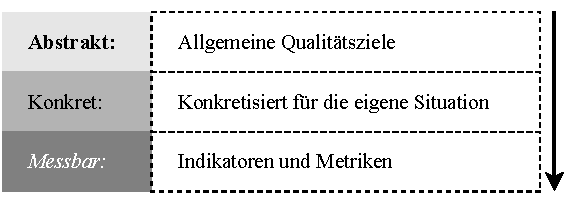
\includegraphics{contents/02_basics/res/quality_models.pdf}
    \caption{Aufbau eines Qualitätsmodells in drei Ebenen \cite[S. 34, ][]{schneider2012abenteuer}}
    \label{fig:basics_quality_models}
\end{figure}

\cite{schneider2012abenteuer}

\chapter{Ziel der Arbeit}

\section{Zieldefinition}

\section{Personas}
1) What are the relevant target groups G, e.g., engineers, end users, or lawyers, and which traits characterize each group’s representatives R, e.g., specific background knowledge or cognitive capacities? 2) What are the explananda X, e.g., events or decisions? 3) Which aspects Y of the explananda X must be explained to which target group G, e.g., why is a decision justified, which causal chain of internal system events led up to it, why did some event e happen instead of event e 4) In which context C may an aspect Y need explanation, and what are the implied constraints? For example, explanations might have to be aural in a driving situation. \cite{kohl_explainability_2019} Die genanten Abhängigkeiten müssen beatnwortet werden.


\section{Forschungsfragen}

\begin{figure}[htb!]
    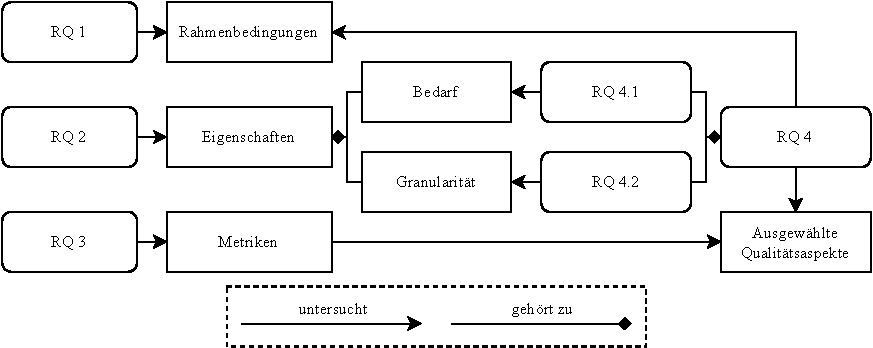
\includegraphics{contents/03_research_design/res/research_questions_overview.pdf}
    \caption{Zusammenhänge der Forschungsfragen}
    \label{fig:research_questions_overview}
\end{figure}

Aus dem Forschungsziel wurden insgesamt fünf Forschungsfragen abgeleitet, welche die Richtung der Arbeit fein granularer definieren. Jede Forschungsfrage behandelt entweder einen konkreten Betrachtungsgegenstand von Erklärbarkeit oder den Zusammenhang dieser einzelnen Aspekte. Wie die einzelnen Forschungsfragen voneinander abhängen, ist in \autoref{fig:research_questions_overview} dargestellt.

\smallskip

\noindent\fbox{
    \parbox{0.965\textwidth}{
        \smallskip
        \textbf{RQ1} Welche Rahmenbedingungen haben einen Einfluss auf die Anforderungen für Erklärungen?
        \smallskip
    }
}

\smallskip

Erklärbare Systeme können sehr verschiedene Ausprägungen haben (z.B. Empfehlungssystem \cite{nunes_systematic_2017} oder Autonome Fahrzeuge \cite{wiegand2019drive}). Auch werden je nach Anwendungsgebiet verschiedene Anforderungen an die Systeme gestellt oder es gibt zusätzlich geltende, äußere Bedingungen \cite{chazette_knowledge_nodate}.

Welche dieser Aspekte einen Einfluss auf die benötigten Erklärungen bzw. Erklärbarkeit im Allgemeinen haben, deckt diese Frage ab. Vor allem konzentriert sich die Frage darauf über welche Rahmenbedingungen sich Stakeholder, die Erklärungen in ein Software-System integrieren möchten, Gedanken machen sollten, um Anforderungen an diese zu formulieren. Dies beinhaltet auch die Ziele, die der Stakeholder für die Software hat.

\smallskip

\noindent\fbox{
    \parbox{0.965\textwidth}{
        \smallskip
        \textbf{RQ2} Welche Eigenschaften von Erklärungen haben einen Einfluss auf die externe Qualität eines erklärbaren Systems?
        \smallskip
    }
}

\smallskip

Es existieren bereits verschiedene Frameworks, welche in bestimmten Kontexten einen Überblick darüber geben, welche Möglichkeiten es gibt, Erklärungen zu gestalten \cite{nunes_systematic_2017}. Vor allem im Bereich der Künstlichen Intelligenz gibt es zahlreiche Arbeiten, welche verschiedene Möglichkeiten vorstellen, um automatisch Erklärungen für komplexe Algorithmen zu generieren \cite{sokol_explainability_2020, mahoney2019framework}.

Um der Forderung nach einem stärkeren Fokus auf den Menschen bei der Betrachtung von Erklärbarkeit nachzukommen \cite{ehsan_operationalizing_2021}, stellt diese Forschungsfrage die externen Qualitätsaspekte \cite{international2011iso} in den Mittelpunkt. Außerdem betrachtet diese Frage die genauen Gestaltungsmöglichkeiten, die Entwicklern oder Designern bei der Konzeption von Erklärungen geboten werden. Folglich ist die Antwort auf diese Frage eine zentrale Grundlage für den Leitfaden, dessen Entwicklung ein Ziel dieser Arbeit ist.

\smallskip

\noindent\fbox{
    \parbox{0.965\textwidth}{
        \smallskip
        \textbf{RQ3} Anhand welcher Metriken kann gemessen werden, ob die in ein erklärbares System integrierten Erklärungen das Ziel der Integration bezogen auf externe Qualitätsaspekte erfüllt haben?
        \smallskip
    }
}

\smallskip

Erklärbarkeit ist eine NFR, welche von vielen verschiedenen Faktoren abhängt und diese auch beeinflusst \cite{chazette_knowledge_nodate}. Die Integration von Erklärungen hat in der Regel Effekte auf mehrere andere Qualitätsaspekte. Diese können sowohl positiv als auch negativ ausfallen. Ein Problem, welches durch die Integration von Erklärungen leicht entstehen kann, ist, dass sich die \textit{Usability} des Systems verschlechtert, wenn sie nicht explizit mitgedacht wird \cite{sokol_explainability_2020}. Folglich stellt das Messen der Qualität von Erklärungen aufgrund der vielfältigen Effekte eine Herausforderung dar. Unterstützt wird dies dadurch, dass viele der durch Erklärbarkeit beeinflussten NFRs vor allem subjektiv von Software-Nutzern wahrgenommen und somit nur wenige objektive Metriken einsetzbar sind \cite{sokol_explainability_2020}.

Zwar wurden in der Literatur bereits Erklärungen anhand verschiedener Metriken analysiert \cite{wiegand2019drive,briand1995goal}. Es fehlt allerdings ein Überblick, welche Metriken zum Messen und zur Bewertung der Qualität von Erklärungen geeignet und erprobt sind. Folglich ist das Ziel bei der Beantwortung dieser offenen Frage, die Metriken, welche bereits zur Evaluation von Erklärungen genutzt wurden, zusammenzutragen.

\smallskip

\noindent\fbox{
    \parbox{0.965\textwidth}{
        \smallskip
        \textbf{RQ4.1} Welchen Einfluss haben der Kontext und die Zielsetzung eines erklärbaren Systems auf den Bedarf für Erklärungen in Bezug auf die externe Qualität des Systems, wenn Erklärungsbedarf besteht?

        \smallskip

        \textbf{RQ4.2} Welchen Einfluss haben der Kontext und die Zielsetzung eines erklärbaren Systems auf die Granularität von Erklärungen in Bezug auf die externe Qualität des Systems, wenn Erklärungsbedarf besteht?
        \smallskip
    }
}

\smallskip

In den ersten drei Forschungsfragen wurden verschiedene Aspekte von Erklärbarkeit behandelt, die wichtig sind, um darauf basierend Erklärungen in ein System zu integrieren. Es fehlt allerdings die Möglichkeit, anhand der Antworten auf diese Fragen eine Auswahl bei der Gestaltung von Erklärungen zu treffen. Eine Antwort auf diese letzten beiden Fragen soll diesen Prozess unterstützen.

Die Einflüsse, nach denen RQ4.1 fragt, sollen bei der Einschätzung helfen, ob und wenn ja, an welchen Stellen ein System Erklärungen benötigt. Dies soll Entwicklern und Designern dabei helfen, die Frage nach dem Bedarf für Erklärungen Anwendungsfall-übergreifend zu beantworten. Für Navigationsanwendungen haben dies beispielsweise \citeauthor{chazette_end-users_nodate} und \citeauthor{wang_integration_2020} bereits getan \cite{chazette_end-users_nodate,wang_integration_2020}.

Wenn eben dieser Bedarf besteht, muss anschließend die Ausgestaltung dieser Erklärung betrachtet werden. Welche bereits untersuchten Einflüsse in Bezug auf diese Granularität von Erklärungen bereits bestehen soll die Antwort auf die Frage RQ4.2 beantworten.

Folglich stellen die Forschungsfragen RQ4.1 und RQ4.2 die Schnittstelle zwischen den ersten drei Forschungsfragen dar.

\bigskip

Die Vorgehensweise dieser Arbeit zum Erreichen des vorgestellten Ziels und bei der Beantwortung der aus dem Ziel abgeleiteten Forschungsfragen wird im folgenden Abschnitt vorgestellt.

\section{Forschungsdesign}
\begin{figure}[htb!]
    \begin{center}
        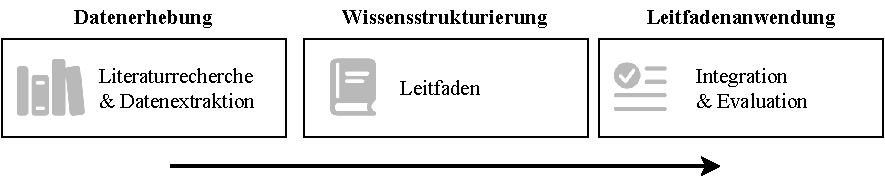
\includegraphics[width=\textwidth]{contents/03_research_design/res/research_design_overview.pdf}
    \end{center}
    \caption{Überblick des Forschungsdesigns}
    \label{fig:research_design_overview}
\end{figure}

Eine Übersicht der Vorgehensweise zur Beantwortung der Forschungsfragen ist in \autoref{fig:research_design_overview} dargestellt. Der Forschungsansatz besteht aus zwei wesentlichen zusammenhängenden Teilen.

Zunächst wurden Daten zum aktuellen Wissensstand über die Aspekte von Erklärungen sowie dessen Zusammenhänge und Auswirkungen auf Softwarequalität erhoben. Zu diesem Zweck wurde eine Literaturrecherche mittels der Suchstring-Methode \cite{kitchenham2004procedures} durchgeführt. Die Antworten auf die Forschungsfragen sind aus den selektierten Arbeiten extrahiert worden, wobei zunächst die Forschungsfragen RQ1 bis RQ3 bearbeitet wurden, um darauf aufbauend die Fragen nach den Einflüssen (RQ4.1 und RQ4.2) zu beantworten.

Auf Basis der Resultate dieser Datenerhebung konnten die Ergebnisse zu den ersten drei Forschungsfragen in ein Modell über die Aspekte von Erklärbarkeit überführt werden. Dies orientiert sich sowohl an Strukturen, welche die Literaturrecherche ergeben hat, als auch an den Forschungsfragen und der Definition von Erklärbarkeit von \citeauthor{chazette_knowledge_nodate} \cite{chazette_knowledge_nodate} (siehe \autoref{sec:model_explanation_aspects}).

Die erhobenen Daten zur Beantwortung der Forschungsfragen RQ4.1 und RQ4.2 sind in einem Katalog der Zusammenhänge zwischen Rahmenbedingen, Charakteristiken von Erklärungen und dem Einfluss auf ausgewählte für Endnutzer wahrnehmbare  Qualitätsaspekte (externe Qualitätsaspekte) gebündelt. Als Schlussfolgerung daraus wurden zusätzlich Design-Empfehlungen abgeleitet.

\bigbreak

Der zweite Teil der Forschung besteht aus der Anwendung des entstandenen Leitfadens. Dies dient der Prüfung, ob der Leitfaden die Integration von Erklärungen in ein bestehendes System unterstützt. Das Ziel ist es, durch neu integrierte Erklärungen positive Auswirkungen auf zuvor definierte Qualitätsziele zu erhalten.

Die Prüfung der Praxistauglichkeit des Leitfadens wurde zusammen mit dem Unternehmen \textit{Graphmasters GmbH} \footnote{\url{https://www.graphmasters.net}, besucht: 10.09.21} aus Hannover durchgeführt. \textit{Graphmasters} ist unter anderem das entwickelnde Unternehmen hinter der Navigationssoftware \textit{NUNAV Navigation} \footnote{\url{https://www.nunav.net}, besucht: 10.09.21}, welches ein Smartphone-Navigationssystem für Endnutzer mit einem kollaborativen Routing-Ansatz ist (Für mehr Details siehe \autoref{sec:model_evaluation}).

Zunächst wurden bestehende Nutzungsprobleme von \textit{NUNAV} analysiert. Darauf basierend hat ein interdisziplinäres Team von \textit{Graphmasters} in einem vorbereiteten Workshop (siehe \autoref{sec:appendix_workshop_protocol}) anhand des zuvor entwickelten Leitfadens grundlegende Ideen für Erklärungen gesammelt. Mithilfe dieser konnten konkrete Anforderungen abgeleitet werden.

Auf Basis der Ergebnisse wurden dann mehrere Erklärungstypen entwickelt und in NUNAV integriert. Diese sind im nächsten Schritt in einer \textit{Case Study} mit Nutzern des Systems evaluiert worden.

Als Abschluss der Forschung wurde zur besseren Interpretation der qualitativen Ergebnisse der \textit{Case Study} ein nicht repräsentatives qualitatives Experiment (Quasi-Experiment) unter Nutzern von \textit{NUNAV Navigation} durchgeführt.

\bigskip

In den folgenden Kapiteln werden die einzelnen beschriebenen Schritte zusammen mit den Ergebnissen näher erläutert.

\chapter{Literaturrecherche}
\label{sec:literature_review}

\section{Definition der Suchbegriffe}
    
% control papers that should appear: \cite{chazette_end-users_nodate} \cite{chazette2020explainability} \cite{kohl_explainability_2019} \cite{sokol_explainability_2020}

\section{Auswahlkriterien für Primärliteratur}



\section{Durchführung}

wichtige zitierte wie \cite{nunes_systematic_2017} wurden trotzdem genommen.

\begin{figure}
    \centering
    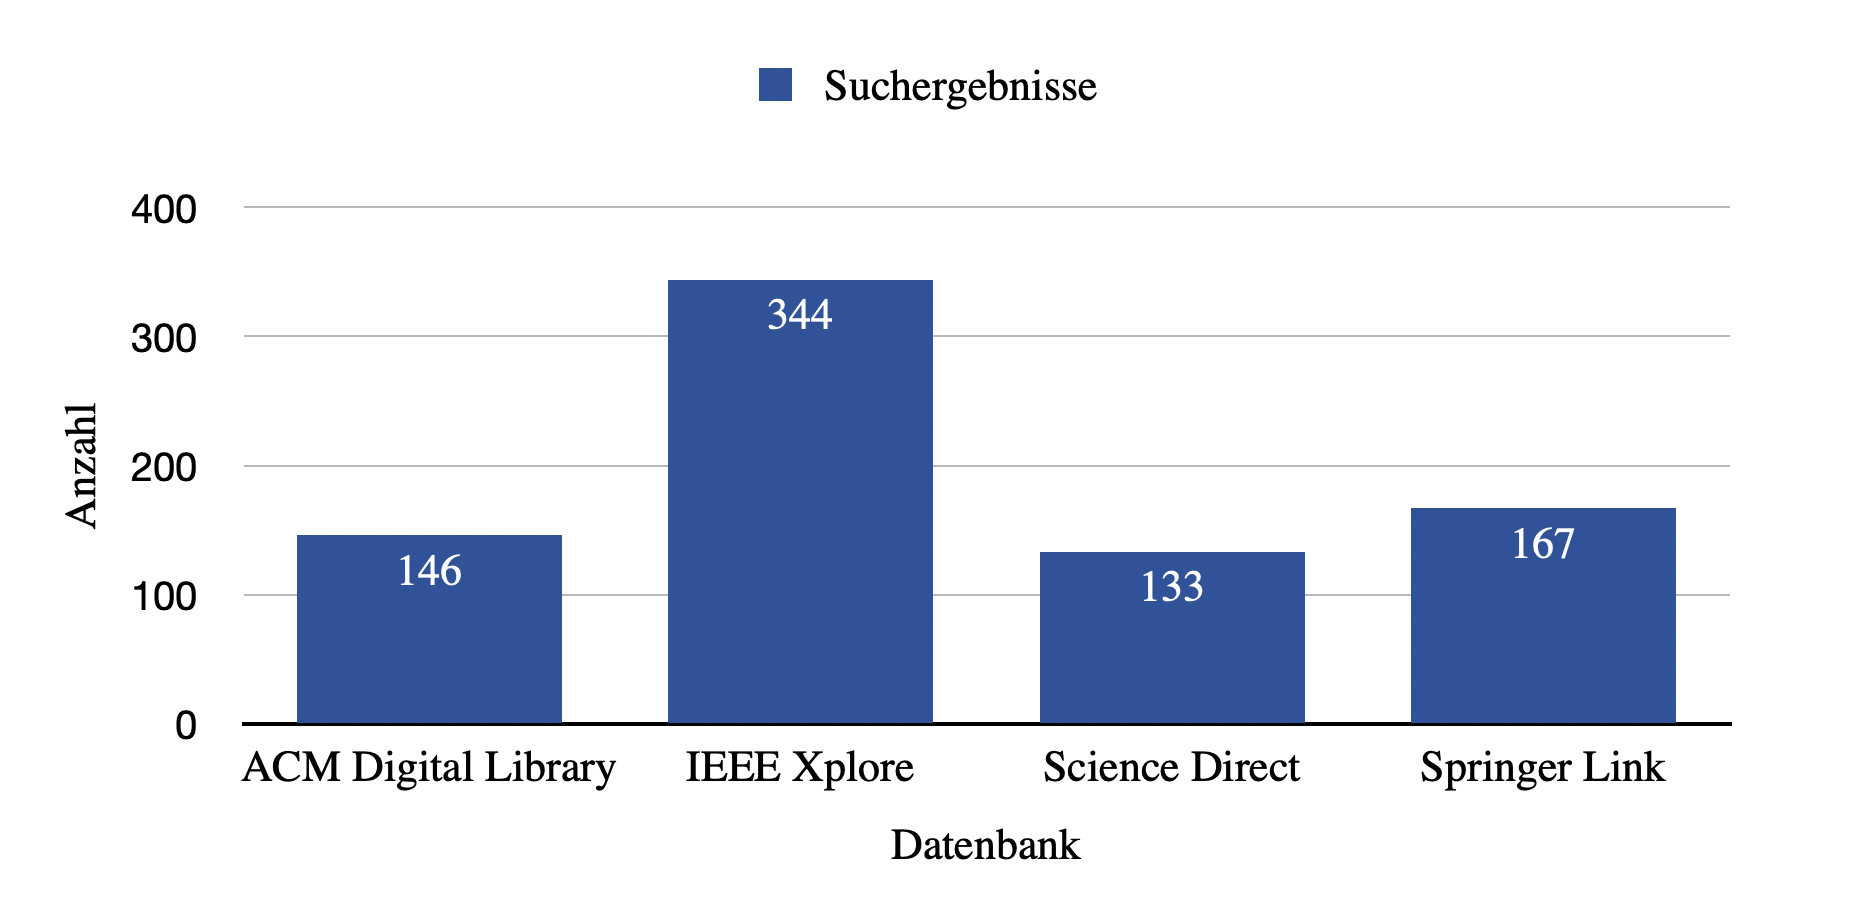
\includegraphics[width=0.75\linewidth]{contents/04_literature_review/res/database_results.png}
    \caption{Anzahl der Suchergebnisse pro Datenbank}
    \label{fig:04_literature_review_screening_process}
\end{figure}

\begin{figure}
    \centering
    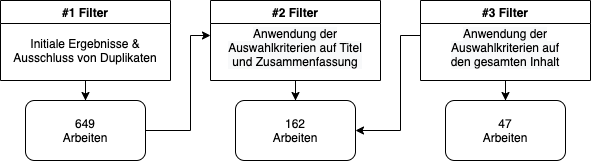
\includegraphics[width=0.8\linewidth]{contents/04_literature_review/res/selection_process.png}
    \caption{Auswahlverfahren der Literaturrecherche}
    \label{fig:04_literature_review_selection_process}
\end{figure}

\pagebreak

\section{Ergebnisse}
%Paper Typen, die am Ende herauskamen:

%Die Paper können in Zwei Kategorien eingeteilt werden: Paper, die 

\begin{table}
    \begin{center}
        \begin{tabular}{p{.3\textwidth}p{.3\textwidth}p{.31\textwidth}}
            \hline
             & Empirische Strategie & Quellen \\
             \toprule
             Evaluation &  & \\
            Qualitätsaspekte                                                                &
            Kontrolliertes Experiment                                                       &
                 \cite{tintarev_designing_nodate} \cite{sato_context_nodate} \cite{eiband_impact_2019} \cite{tsai_evaluating_2019} \cite{hernandez-bocanegra_effects_2020} \cite{balog_measuring_2020} \cite{kunkel_let_2019} \cite{schaffer_i_2019} \cite{weitz_you_2019} \cite{yamada_evaluating_2016} \cite{sato_action-triggering_2019} \cite{haspiel_explanations_2018} \cite{zahedi_towards_2019} \cite{zolotas_towards_2019} \cite{riveiro_thats_2021}  \cite{martin_evaluating_2021} \cite{tsai_effects_2020}    \cite{neerincx_using_2018} \cite{schrills_color_2020} \cite{wang_is_2018} \cite{zhu_effects_2020} \cite{koo_why_2015} \cite{koo_understanding_2016} \cite{cheng2019explaining}
                 \\
                                                                                            &
            Case Study                                                                      &
                 \cite{martin_developing_2019} \cite{ehsan_human-centered_2020}
                 \\
                                                                                            &
            Umfrage                                                                         &
                \cite{chazette_end-users_nodate} \cite{chazette2020explainability} \cite{sokol_one_2020}
            \\
            Nutzer-Präferenz                                                                &
            Kontrolliertes Experiment                                                       &
                \cite{kouki_user_2017} \cite{mucha_interfaces_2021} \cite{abdulrahman_belief-based_2019} \cite{waa_evaluating_2021} \cite{wiegand_id_2020} \cite{stange_effects_2021} \cite{kaptein_personalised_2017} \cite{wiegand2019drive} \cite{du2019look}
            \\
            \midrule
            Analyse &  & \\
            Überblick                                                                       &
            Literaturrecherche                                                              &
                \cite{chazette_knowledge_nodate} \cite{sokol_explainability_2020} \cite{tintarev2015explaining} \cite{kohl_explainability_2019} \cite{rosenfeld_explainability_2019} \cite{cassens_ambient_2019} \cite{cirqueira_scenario-based_2020} \cite{rjoob_towards_2021} \cite{thomson_knowledge--information_2020} \cite{chari_explanation_2020} \cite{nunes_systematic_2017} \cite{sovrano_modelling_2020} \cite{ribera2019can} \cite{gunning2019darpa} \cite{doshi2017towards} \cite{lim_2009_assessing} \cite{tintarev2007survey}
                \\
                                                                                            &
            Umfrage                                                                         &
                \cite{brennen_what_2020} 
            \\ \toprule
        \end{tabular}
    \end{center}
    \caption{Ergebnisse der Literaturrecherche nach Art der Publikation}
    \label{tab:results_paper_types}
\end{table}

\begin{table}
    \begin{center}
        \begin{tabular}{p{.3\textwidth}p{.64\textwidth}}
            \hline
            Kontext                   & Quellen \\
            \toprule
            Allgemein                           &
                \cite{chazette_end-users_nodate} \cite{chazette2020explainability} \cite{chazette_knowledge_nodate} \cite{eiband_impact_2019} \cite{kohl_explainability_2019} \cite{ribera2019can} \cite{lim_2009_assessing} \\
            \tablerowspacing
            Intelligente Systeme (z.B. XAI)      & 
                \cite{waa_evaluating_2021} \cite{mucha_interfaces_2021} \cite{sokol_explainability_2020}  \cite{abdulrahman_belief-based_2019} \cite{brennen_what_2020} \cite{schaffer_i_2019} \cite{weitz_you_2019} \cite{riveiro_thats_2021} \cite{martin_developing_2019} \cite{martin_evaluating_2021} \cite{rosenfeld_explainability_2019} \cite{cassens_ambient_2019} \cite{cirqueira_scenario-based_2020}  \cite{ehsan_human-centered_2020} \cite{rjoob_towards_2021} \cite{thomson_knowledge--information_2020} \cite{chari_explanation_2020} \cite{sokol_one_2020}  \cite{neerincx_using_2018} \cite{schrills_color_2020} \cite{sovrano_modelling_2020} \cite{gunning2019darpa} \cite{doshi2017towards} \cite{cheng2019explaining}\\
            \tablerowspacing
            Empfehlungssysteme                  & 
                \cite{tintarev_designing_nodate} \cite{sato_context_nodate} \cite{balog_measuring_2020}  \cite{kouki_user_2017} \cite{tsai_evaluating_2019} \cite{hernandez-bocanegra_effects_2020} \cite{kunkel_let_2019} \cite{tintarev2015explaining} \cite{sato_action-triggering_2019} \cite{tsai_effects_2020} \cite{nunes_systematic_2017} \cite{tintarev2007survey}
            \\
            \tablerowspacing
            Autonomes Fahren                    &
                \cite{wiegand_id_2020} \cite{haspiel_explanations_2018} \cite{koo_understanding_2016} \cite{koo_why_2015} \cite{wiegand2019drive} \cite{du2019look}
            \\
            \tablerowspacing
            Mensch-Roboter-Interaktion          &
                \cite{stange_effects_2021} \cite{kaptein_personalised_2017} \cite{zolotas_towards_2019} \cite{wang_is_2018} \cite{zhu_effects_2020}
            \\
            \tablerowspacing
            Domain-Specific                     &
                \cite{yamada_evaluating_2016} \cite{zahedi_towards_2019}
            \\
            \toprule
        \end{tabular}
    \end{center}
    \caption{Kontext innerhalb von Erklärbaren Systemen, der von den Arbeiten untersucht wurde}
    \label{tab:paer_explanation_contexts}
\end{table}



\chapter{Leitfaden zur Integration von Erklärungen}

Das folgende Kapitel beschreibt den Leitfaden zur Integration von Erklärungen, welcher auf Basis der vorangegangenen Literaturrecherche entwickelt wurde (Siehe \autoref{sec:literature_review}). Zuerst werden die konkreten Anforderungen vorgestellt, welche in vorangegangener Literatur erarbeitet wurden, die für einen Leitfaden dieser Art gelten sollten. Neben einem Überblick über die verschiedenen Einflussfaktoren, die bei der Entwicklung von Erklärungen für ein erklärbares System betrachtet werden sollten, gibt \autoref{sec:model_explanation_aspects} außerdem einen Überblick über die Ausprägungen der Eigenschaften von Erklärungen, die in der Literatur bereits Anwendung gefunden haben. Die Evaluation von Erklärungen wird in \autoref{sec:model_evaluation_description} thematisiert. \autoref{sec:model_proved_relations} enthält eine Übersicht von bereits gezeigten Zusammenhängen zwischen bestimmten Aspekten von Erklärungen basierend auf dem Modell der verschiedenen Aspekte von Erklärbarkeit. Abschließend werden in diesem Kapitel die Auswirkungen daraus für das Design von Erklärungen vorgestellt (\autoref{sec:model_design_implications}).

% \smallskip
% 
% Der finale Leitfaden als gekapseltes ARtefakt ohne erläuterungen zur Herkunft ist im Anhang zu finden (\autoref{appendix.....}).

\section{Anforderungen}

Nach einer Untersuchung von Erklärungen stellen mehrere Autoren den Bedarf für eine Vereinheitlichung der Untersuchung von Erklärungen fest \cite{cirqueira_scenario-based_2020,zahedi_towards_2019, nunes_systematic_2017, martin_evaluating_2021}. Dies soll es ermöglichen, den Vergleich zwischen verschiedenen Lösungsansätzen zu vereinfachen. In einigen Arbeiten fordern die Autoren, dass ein einheitliches Framework zur Evaluation benötigt wird, anhand dessen die Qualität von Erklärungen bestimmt werden kann \cite{nunes_systematic_2017,sokol_explainability_2020,chari_explanation_2020}. Allerdings wird auch darauf verwiesen, dass es einer Unterstützung bedarf, um Anforderungen an die Erklärungen zu formulieren bzw. die Probleme, welche durch Erklärungen gelöst werden sollen zu identifizieren \cite{chazette_end-users_nodate, doshi2017towards}. Unterstützt wird dies durch \citeauthor{waa_evaluating_2021}, welche dies nutzen wollen, um jeder Prüfung von Erklärungen klare Hypothesen voraus zustellen, um die Ergebnisse verschiedener Arbeiten besser zusammenfassen und daraus Empfehlungen ableiten zu können. Auch \citeauthor{kohl_explainability_2019} unterstreicht den Aspekt, dass vor allem die Ziele und Anforderungen auf Basis des aktuellen Kontextes klar sein müssen, bevor Erklärungen in ein System integriert werden. Folglich sollte das Modell auch hierfür Unterstützung bieten. Außerdem ergibt sich aus dem Ziel der Arbeit (\autoref{sec:goal_definition}), dass das Modell auch Gestaltungsempfehlungen für Erklärungen enthalten und somit einen Teil der Forderung von \citeauthor{waa_evaluating_2021} nach einem Überblick über bisherige Ergebnisse erfüllen soll. Basis hierfür sind die Forschungsfragen RQ2 und RQ3, welche nach den Auswirkungen verschiedener Eigenschaften von Erklärungen fragen. Voraussetzung dafür ist allerdings auch, dass mögliche Eigenschaften von Erklärungen definiert werden (RQ1).

Zusammenfassend kann man also sagen, dass dieses Modell vor allem drei Aspekte erfüllen muss:

\begin{enumerate}
    \item Das Modell muss das Erheben von Anforderungen an Erklärungen und das Aufstellen von Hypothesen über den Einfluss vereinfachen.
    \item Im Modell sollten die bereits evaluierten möglichen Formen von Erklärungen dargestellt werden.
    \item Das Modell muss einen Überblick über verschiedene Evaluationsmöglichkeiten geben, um die Qualität von integrierten Erklärungen im Nachhinein zu bewerten.
    \item Es müssen existente Ergebnisse aus der Literatur so im Modell zusammengefasst sein, dass es für einen Nutzer des Modells möglich ist, diese auf seinen Kontext zu übertragen und folglich Erklärungen in ein System zu integrieren.
\end{enumerate}

\section{Aspekte von Erklärungen}
\label{sec:model_explanation_aspects}

Literatur, die einen Überblick über Erklärbarkeit im Allgemeinen oder in einem bestimmten Anwendungsfeld gibt, betrachtet in der Regel fünf Aspekte von Erklärbarkeit \cite{rosenfeld_explainability_2019, nunes_systematic_2017,chazette_knowledge_nodate}. Dies sind der Kontext der Erklärung, die Zielsetzung dieser, welche Erklärung angezeigt werden soll und wann diese angezeigt werden soll. In einigen Arbeiten wird bei der angezeigten Erklärung außerdem zwischen dem Inhalt und der Darstellung unterschieden bzw. diese Eigenschaften einzeln untersucht \cite{nunes_systematic_2017,abdulrahman_belief-based_2019}. Darüber hinaus wird in allen hier betrachteten Arbeiten auch die Evaluation von Erklärungen thematisiert (Siehe \autoref{sec:literature_review}).

Für die zuvor genannten Aspekte werden in der Literatur verschiedene Unterkategorien konkret benannt oder Synonyme verwendet. \autoref{tab:model_explaination_aspects} fasst die verwendeten Synonyme aus den Veröffentlichungen, welche den Aspekt explizit erwähnt haben, unter der final gewählten Benennung zusammen. Neben den dort aufgezeigten Begriffen haben mehrere Autoren (z.~B. \cite{rosenfeld_explainability_2019, chazette2020explainability}) die verschiedenen Aspekte von Erklärbarkeit zusätzlich mit Fragewörtern verknüpft. Die vollständigen Fragen dahinter verweisen allerdings auf verschiedene Unterpunkte, weswegen das vorgestellte Modell auf Fragewörter verzichtet, um Verwechselungen vorzubeugen. (Beispiel: \glqq \textbf{Wie} kann die Erklärung evaluiert werden?\grqq{} (\textit{Evaluation}) \cite[vgl.][]{rosenfeld_explainability_2019} und \glqq \textbf{Wie} viele Informationen sollte jede Erklärung enthalten?\grqq{} (\textit{Content}) \cite[vgl.][]{kouki_user_2017}).

\bigskip

Im Folgenden werden die genannten Oberkategorien erläutert bzw. definiert.

\begin{table}
    \begin{tabular}{|p{.2\textwidth}|p{.4\textwidth}|p{.3\textwidth}|}
        \hline
        \textbf{Aspekt} & \textbf{Synonyme}         & \textbf{Quellen} \\ \hline
        1. Context      & (Experimental) Context    & \cite{chazette_knowledge_nodate} \cite{chazette_end-users_nodate}
                                                    \cite{sato_context_nodate} \cite{waa_evaluating_2021} 
                                                    \cite{kohl_explainability_2019} \cite{neerincx_using_2018} 
                                                    \cite{sovrano_modelling_2020} \cite{doshi2017towards} \\
                        & (Explanation) Scope       & \cite{wohlin2012experimentation} \cite{eiband_impact_2019}
                                                    \cite{doshi2017towards} \\
                        & Use Case                  & \cite{waa_evaluating_2021} \\
                        & Stakeholder               & \cite{rosenfeld_explainability_2019} \\
        \hline
        2. Objectives   & Objectives                & \cite{nunes_systematic_2017} \\
                        & Construct                 & \cite{waa_evaluating_2021} \\
                        & Purpose                   & \cite{nunes_systematic_2017} \cite{wohlin2012experimentation} \\
                        & (Stakeholder) Goals       & \cite{cirqueira_scenario-based_2020}
                                                    \cite{sovrano_modelling_2020} \cite{ribera2019can} \\
                        & Main Drive                & \cite{anjomshoae2019explainable} \\
                        & Intended Effect           & \cite{balog_measuring_2020} \\
        \hline
        3. Demand       & Demand                    & \cite{chazette_knowledge_nodate} \\
        \hline
        4. Content      & User Interface Component(s) & \cite{nunes_systematic_2017}
                                                    \cite{rosenfeld_explainability_2019} \\
                        & Content                   & \cite{ribera2019can} \\
                        & Granularity               & \cite{chazette_knowledge_nodate}
                                                    \cite{kohl_explainability_2019} \\
        \hline
        5. Presentation & Presentation              & \cite{rosenfeld_explainability_2019} \cite{kouki_user_2017} \\
                        & (Explanation) Type        & \cite{ribera2019can} \cite{rosenfeld_explainability_2019} \\
        \hline
        6. Evaluation   & Evaluation                & \cite{kohl_explainability_2019} \cite{doshi2017towards} \\
                        & Measurements              & \cite{waa_evaluating_2021} \cite{balog_measuring_2020} \\
                        & Metrics                   & \cite{nunes_systematic_2017} \cite{anjomshoae2019explainable}
                                                    \cite{chari_explanation_2020} \cite{waa_evaluating_2021}\\
        \hline
    \end{tabular}
\caption{Übergeordnete Aspekte von Erklärungen in der Literatur}
\label{tab:model_explaination_aspects}
\end{table}

\paragraph{Context} Der \textit{Context} einer Erklärung wird durch die Situation gegeben, welche durch die Interaktion eines Nutzers, seiner Aufgabe, dem System und der Umgebung entsteht. (\cite[vgl.][]{chazette_knowledge_nodate, kohl_explainability_2019}).

\paragraph{Objectives} \textit{Objectives} sind die Qualitätsziele, welche für eine Erklärung gelten oder aufgrund derer Erklärungen in ein System integriert werden sollen.

\paragraph{Demand} Der \textit{Demand} für eine Erklärung ist der Bedarf für Erklärungen durch den Nutzer eines Systems. Das heißt der \textit{Demand} beschreibt die Notwendigkeit, zu einemen bestimmten Zeitpunkt für einen Systemteil Erklärungen bereitzustellen. Das beinhaltet auch, ob die Initiative vom Nutzer ausgeht oder das System selbstständig eine Erklärung anzeigt.

\paragraph{Content} Der \textit{Content} einer bei bestehendem Bedarf dem Nutzer bereitgestellten Erklärung ist durch die Informationen und die Informationsdichte definiert.

\paragraph{Presentation} Der Inhalt einer Erklärung kann Nutzern auf verschiedenen Wegen zugänglich gemacht werden. Die \textit{Presentation} einer Erklärung ist die Art und Weise, auf die dem Nutzer die Informationen durch die Erklörung bereitgestellt werden.

\paragraph{Evaluation} Die \textit{Evaluation} ist die Bewertung der Qualität von Erklärungen. Dies enthält die grundsätzlichen verschiedenen Evaluationsmöglihckeiten und- Metriken mit denen die Qualität gemessen werden kann.

\subsection{Struktur des Modells}

Die Struktur des Modells für Erklärungen orientiert sich an den Forschungsfragen und Anforderungen an das Modell, Ergebnissen aus der Literaturrecherche sowie dem bestehenden Konzept der Qualitätsmodelle \cite{schneider2012abenteuer} (Siehe \autoref{sec:basics_quality_models}).

In der Literatur wurden einige Aspekte des Modells nicht nur verschieden genannt, sondern auch zum Teil in Oberkategorien gegliedert oder auf verschiedenen Abstraktionsebenen betrachtet. Hieraus ergibt sich eine Hierarchische Anordung des Modells. Verschiedene Abstraktionsebenen enthalten auch die von \citeauthor{schneider2012abenteuer} vorgestellten Qualitätsmodelle \cite{schneider2012abenteuer}. Dabei werden abstrakte Ziele (\textit{Objectives}) immer weiter konkretisiert, bis sie schlussendlich mit konkreten Metriken messbar sind. Das zugrunde liegende Modell (\glqq Goal-Driven and Property-Based Definition Approach for Product Metrics\grqq{} \cite{briand1995goal}) von \citeauthor{briand1995goal} definiert außerdem unter anderem die nötigen Abhängigkeiten der \textit{Objectives} von äußeren Faktoren, die im hier vorgestellten Modell für Erklärungen dem bereits erwähnten \textit{Context} entsprechen.

Die Betrachtung von \textit{Context} und \textit{Objectives} erfolgt in der Literaur über Erklärungen zum Teil in verschiedener Reihenfolge. \citeauthor{rosenfeld_explainability_2019} schreiben, dass die erste Frage, welche geklärt werden sollte, die Frage \glqq Warum benötigt das System eine Erklärung?\grqq{} ist \cite[vgl. S. 699][]{rosenfeld_explainability_2019}\cite{nunes_systematic_2017}. Im Gegensatz dazu schreiben \citeauthor{cirqueira_scenario-based_2020}, dass zuerst äußere Umstände, wie der Endnutzer des Systems geklärt sein sollte (\glqq Stakeholder Setting\grqq{} \cite{cirqueira_scenario-based_2020}), um darauf aufbauend die Ziele festzulegen. Hieraus wird geschlussfolgert, dass die Festlegung der Ziele mit ihren Abhängigkeiten wie auch von \cite{schneider2012abenteuer} geschildert eine iterative, stark zusammenhängende Aufgabe ist. Daher werden die Punkte \textit{Context} und \textit{Objectives} aus \autoref{tab:model_explaination_aspects} unter \textit{External Dependencies} zusammengefasst. Dies verdeutlicht, dass die \textit{Objectives} für das Integrieren von Erklärungen stark mit anderen äußeren Einflüssen (\textit{Context}) zusammenhängen (\autoref{sec:model_external_dependencies}).

Auch werden \textit{Demand}, \textit{Content} und \textit{Presentation} vereint dargestellt, da sich diese drei Kategorien direkt auf die Eigenschaften von Erklärungen beziehen (\textit{Characteristics}). Damit wird der Zusammenhang zwischen den verschiedenen Merkmalen einer Erklärung verdeutlicht \cite{nunes_systematic_2017}.

Zusätzlich zur Zielevaluation von Qualitätsmodellen betrachtet das vorgestellte Modell die unmittelbare Evaluation von Erklärungen. Diese müssen einzeln betrachtet werden, da für diese die Metriken zum Teil erst nach der Entwicklung der Erklärungen festgelegt werden können.

\smallbreak

Schlussendlich ist das Modell in die drei Oberkategorien \textit{External Dependencies}, \textit{Characteristics} und \textit{Evaluation} gegliedert. Eine Übersicht ist in \autoref{fig:model_overview} zu sehen. Die Gesamtübersicht des Modells für Erklärungen bietet \autoref{fig:model_overview_complete}. Diese enthält darüber hinaus die in den folgenden Abschnitten beschriebenen Ausprägungen der einzelnen Kategorien aus der Literatur. Die Gesamtübersicht ist grafisch an der Taxonomie für Erklärungen von \citeauthor{nunes_systematic_2017} angelehnt und enthält auch einige Aspekte daraus \cite{nunes_systematic_2017}. Die erwähnte Taxonomie ist allerdings nur auf den Einsatz von Erklärungen in Empfehlungssystemen bezogen und beschränkt sich daher u.~a. auf bestimmte Darstellungstypen. Sie kann folglich nicht ohne Weiteres in andere Kontexte übertragen werden. Darüber hinaus fehlt der Aspekt der Evaluation. Dieser wird allerdings nicht nur von \citeauthor{nunes_systematic_2017} selbst, sondern auch von weiteren Autoren für wichtig erachtet \cite{cirqueira_scenario-based_2020, martin_evaluating_2021}.

\begin{figure}[htb!]
    \begin{center}
        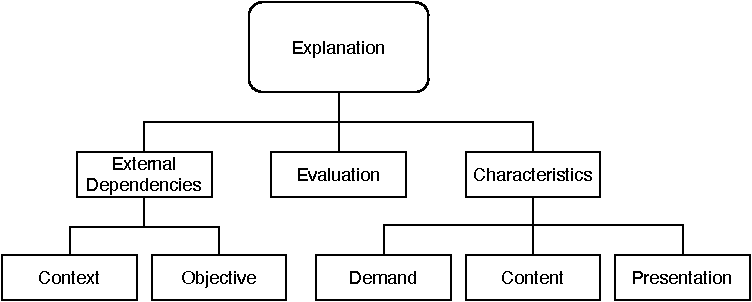
\includegraphics[width=0.9\linewidth]{contents/05_model_description/res/model-overview.pdf}
    \end{center}
    \caption{Oberkategorien der Aspekte von Erklärungen}
    \label{fig:model_overview}
\end{figure}

\subsection{Externe Abhängigkeiten}
\label{sec:model_external_dependencies}

Unter \textit{External Dependencies} sind die Aspekte zusammengefasst, die eine Auswirkung auf Erklärungen in einem System haben. Außerdem können von den hier aufgeführten Punkten Anforderungen abgeleitet und später zusammen mit Metriken Hypothesen aufgestellt werden. Daraus kann dann auch abgeleitet werden, welche Funktionen des Systems einer Erklärung bedürfen \cite{kohl_explainability_2019}.

Wie bereits beschrieben, sind die \textit{External Dependencies} in den \textit{Context} und die \textit{Objectives} unterteilt. Über die Reihenfolge, in der ein Stakeholder, der Erklärungen in ein System integrieren möchte, die beiden Aspekte betrachten sollte, gibt es in der Literatur unterschiedliche Meinungen. \citeauthor{rosenfeld_explainability_2019} schreiben, dass die erste Frage, welche geklärt werden sollte, die Frage \glqq Warum benötigt das System eine Erklärung?\grqq{} ist \cite[vgl. S. 699][]{rosenfeld_explainability_2019}. Im Gegensatz dazu schrieben \citeauthor{cirqueira_scenario-based_2020}, dass zuerst äußere Umstände, wie der Endnutzer des Systems geklärt sein sollte (\glqq Stakeholder Setting\grqq{} \cite{cirqueira_scenario-based_2020}), um darauf aufbauend die Ziele festzulegen. Laut \citeauthor{briand1995goal} hat zumindest auf die Ziele einer Evaluation der Kontext des Systems einen Einfluss und sollte somit zuvor geklärt werden \cite{briand1995goal}. Aus den verschiedenen Ansichten wird gefolgert, dass der \textit{Context} des Systems und die \textit{Objectives} eng zusammen hängen und nur gemeinsam betrachtet werdeb können.

\subsubsection{Context}

Der \textit{Context} einer Erklärung beschreibt die äußeren Einflüsse, die unmittelbar auf das erklärbare System wirken und somit Anforderungen an die Eigenschaften von Erklärungen stellen.

Dies beinhaltet die Aktivität, die der Endbenutzer in einer bestimmten Umgebung durchführt. Aus den Eigenschaften der drei genannten Aspekte leiten sich dabei direkte Einflüsse auf den Bedarf, den Inhalt und die Darstellung einer Erklärung ab.

In der

Der Begriff Stakeholder wurde hier verschieden eingesetzt. Beispielsweise nutzen \citeauthor{cirqueira_scenario-based_2020}den Begriff für den Nutzer einer Software \cite{cirqueira_scenario-based_2020} und \cite{nunes_systematic_2017} als Oberbegriff für Personengruppen, die ein Interesse an einem System haben, den Nutzer allerdings ausschließen \cite{nunes_systematic_2017}. Diese Arbeit geht von der Definition nach (Quelle suchen) aus, welch alle interessieren Gruppen beschreibt. 

Das Modell von \cite{nunes_systematic_2017} enthält allerdings weder den Kontext noch den Evaluationspart, welcher für einen Überblick über Erklärbarkeit wichtig ist. Der Fokus ist eher auch auf Recommender Systems gelegt

Nur die Kontexte, die explizit erwähnt wurden in \autoref{tab:impact_of_context_on_explanation}

\begin{table}
    \begin{tabular}{|p{.2\textwidth}|p{.5\textwidth}|p{.2\textwidth}|}
        \hline
        \textbf{Aspekt} & \textbf{Synonyme} & \textbf{Quellen} \\ \hline
        End User        &  (Targt / End)  User & \cite{chazette2020explainability} \cite{kaptein_personalised_2017} \cite{sokol_one_2020} \cite{wiegand_id_2020} \\
                        & Stakeholder & \cite{chazette_knowledge_nodate} \\
                        & Consumer & \cite{ehsan_human-centered_2020} \\
                        & Explainee & \cite{chazette_knowledge_nodate} \cite{kohl_explainability_2019} \\
        \hline
        Environment     & Environment & \cite{chazette_knowledge_nodate} \cite{wiegand_id_2020} \cite{wiegand2019drive} \\
                        & Application Area & \cite{sokol_explainability_2020} \cite{wiegand2019drive} \cite{wiegand_id_2020} \\
        \hline
        Task            & Task & \cite{chazette_knowledge_nodate} \cite{sokol_explainability_2020} \cite{gunning2019darpa} \\
                        & Activity & \cite{wohlin2012experimentation} \\
                        
        \hline
    \end{tabular}
    \caption{Kontext einer Erklärung}
    \label{tab:impact_of_context_on_explanation}
\end{table}

\paragraph{Endnutzer}

Different synonyms for it like....

\paragraph{Äußere Bedingungen}

\paragraph{Aufgabe}

\subsubsection{Zielsetzung}
\label{subsec:model_objective}

\cite{chazette_knowledge_nodate} haben einen Katalog zusammengestellt, der die Einflüsse von Erklärbarkeit darstellt

\cite{tintarev_designing_nodate} haben Messliste gebaut.

Nur Erwähnung, wenn das Paper den Aspekt explizit untersucht / erwähnt. In \autoref{tab:quality_aspects_of_explanation} sind alle Arbeiten aufgelistet, die Erklärbarkeit entweder im Bezug auf den aufgelisteten Qualitätsaspekt untersuchen oder 

\begin{table}
    \begin{center}
        \begin{tabular}{|p{.24\textwidth}|p{.5\textwidth}|p{.2\textwidth}|}
            \hline
            \textbf{Qualitätsaspekt}    & \textbf{Beschreibung} & \textbf{Quellen} \\ \hline
            Transparency                & Erklärung, wie das System funktioniert.
                                        & \cite{nunes_systematic_2017} \cite{chazette_knowledge_nodate} \cite{tintarev_designing_nodate} \cite{chazette_end-users_nodate} \cite{balog_measuring_2020} \cite{chazette2020explainability} \cite{tintarev2015explaining} \cite{hernandez-bocanegra_effects_2020} \cite{tsai_effects_2020} \cite{rjoob_towards_2021}  \cite{sokol_one_2020} \cite{wang_is_2018} \cite{koo_understanding_2016} \cite{tintarev2007survey}\\ \hline
            Understandability           & ggf. löschen, da Transparency SIG / Mental Model
                                        & \cite{chazette_knowledge_nodate} \cite{chazette_end-users_nodate} \cite{martin_evaluating_2021}  \cite{ehsan_human-centered_2020} \cite{rjoob_towards_2021}  \cite{sokol_one_2020} \cite{cheng2019explaining} \\ \hline
            Trust                       & Das Vertrauen des Nutzers in das System erhöhen.
                                        & \cite{nunes_systematic_2017} \cite{chazette_knowledge_nodate} \cite{tintarev_designing_nodate} \cite{balog_measuring_2020} \cite{eiband_impact_2019} \cite{tintarev2015explaining} \cite{hernandez-bocanegra_effects_2020} \cite{stange_effects_2021} \cite{weitz_you_2019} \cite{yamada_evaluating_2016} \cite{haspiel_explanations_2018} \cite{martin_developing_2019} \cite{martin_evaluating_2021} \cite{tsai_effects_2020}  \cite{sokol_one_2020}  \cite{wang_is_2018} \cite{koo_understanding_2016} \cite{wiegand2019drive} \cite{gunning2019darpa} \cite{lim_2009_assessing} \cite{tintarev2007survey} \cite{kunkel_let_2019} \\ \hline
            Satisfaction                & Benutzerfreundlichkeit und generelle Zufriedenheit mit dem System erhöhen.
                                        & \cite{nunes_systematic_2017} \cite{chazette_knowledge_nodate} \cite{tintarev_designing_nodate} \cite{balog_measuring_2020} \cite{tsai_evaluating_2019} \cite{tintarev2015explaining} \cite{riveiro_thats_2021} \cite{martin_developing_2019} \cite{martin_evaluating_2021} \cite{tsai_effects_2020} \cite{ehsan_human-centered_2020} \cite{sovrano_modelling_2020} \cite{koo_understanding_2016} \cite{ribera2019can} \cite{gunning2019darpa} \cite{lim_2009_assessing}  \cite{tintarev2007survey} \cite{sato_context_nodate} \\ \hline
            Scrutability                & Dem Nutzer die Möglichkeit geben, dem System einen Fehler mitzuteilen 
                                        & \cite{nunes_systematic_2017} \cite{chazette_knowledge_nodate} \cite{tintarev_designing_nodate} \cite{balog_measuring_2020} \cite{tintarev2015explaining} \cite{martin_developing_2019} \cite{gunning2019darpa}  \cite{tintarev2007survey} \cite{martin_evaluating_2021} \\ \hline
            Efficiency                  & Das Verhältnis von Qualität und Zeit für das Lösen einer Aufgabe verbessern.
                                        & \cite{nunes_systematic_2017} \cite{chazette_knowledge_nodate} \cite{tintarev_designing_nodate} \cite{balog_measuring_2020} \cite{tsai_evaluating_2019} \cite{tintarev2015explaining} \cite{hernandez-bocanegra_effects_2020} \cite{tintarev2007survey}\\ \hline
            Effectiveness               & Die Qualität der Aufgabe des Nutzers erhöhen
                                        & \cite{nunes_systematic_2017} \cite{chazette_knowledge_nodate} \cite{tintarev_designing_nodate} \cite{balog_measuring_2020} \cite{tintarev2015explaining} \cite{zolotas_towards_2019} \cite{hernandez-bocanegra_effects_2020} \cite{martin_evaluating_2021} \cite{rjoob_towards_2021} \cite{tintarev2007survey} \\ \hline
            Persuasiveness              & Convince Users to try or by. \cite{balog_measuring_2020}
                                        & \cite{nunes_systematic_2017} \cite{tintarev_designing_nodate} \cite{balog_measuring_2020} \cite{sato_context_nodate} \cite{sato_context_nodate} \cite{abdulrahman_belief-based_2019} \cite{tintarev2015explaining} \cite{sato_action-triggering_2019} \cite{tintarev2007survey} \\ \hline
        \end{tabular}
    \end{center}
    \caption{Qualitätsaspekte einer Erklärung}
    \label{tab:quality_aspects_of_explanation}
\end{table}

1. To justify its decisions so the human participant can decide to accept them (provide control) 2. To explain the agent’s choices to guarantee safety concerns are met 3. To build trust in the agent’s choices, especially if a mistake is suspected or the human operator does not have experience with the system 4. To explain the agent’s choices to ensure fair, ethical, and/or legal decisions are made 5. Knowledge/scientific discovery 6. To explain the agent’s choices to better evaluate or debug the system in previously unconsidered situations \cite{rosenfeld_explainability_2019}

Usability beschreibt die Qualität einer Erklärung im Bezug auf die Interaktion und die Darstellung Darstellung der Inhalte \cite{chazette_end-users_nodate}. Informativeness ist dierekt bezogen auf den Inhalt der Erklärung \cite{chazette_end-users_nodate}. Direkt messbar an der Erklärung selbst.

\cite{schneider2012abenteuer} beschreibt den Prozess von abstrakten allgemein definierten und bekannten Qualitätszielen hin zu konkreten Metriken. Als Zwischenstufe werden konkrete Qualitätsziele, die für den aktuellen Anwendungsfall gültig sind aufgestellt. \cite{nunes_systematic_2017} und \cite{waa_evaluating_2021} unterteilen diese verschiedenen Abstraktionsebenen der Ziele für Erklärungen in drei Ebenen. Die ursprünglichen Begrifflichkeiten der beiden erwähnten Arbeiten sowie weitere Synonyme aus anderen Arbeiten sind in \autoref{tab:impact_of_objective_on_explanation} zusammengefasst.

7 Established goals von \cite{tintarev2015explaining, tintarev_designing_nodate}

Einteilung in Oberkategorien...

\begin{longtable}{|p{.2\textwidth}|p{.5\textwidth}|p{.2\textwidth}|}
    \hline
    \textbf{Aspekt}     & \textbf{Synonym} & \textbf{Quellen} \\ \hline
    Business Goals      & Motivation & \cite{nunes_systematic_2017} \\
                        & Stakeholder Goals & \cite{nunes_systematic_2017} \\
                        & (Intended) Purpose & \cite{waa_evaluating_2021} \\
                        & Higher-level Goals & \cite{nunes_systematic_2017} \\
                        & Application Level & \cite{sokol_explainability_2020} \\
    \hline
    Users' Perception   & User Perceived Quality Factors & \cite{nunes_systematic_2017} \\
                        & (Consumer) Needs & \cite{ehsan_human-centered_2020} \cite{chazette_end-users_nodate} \\
                        & User Goals & \cite{ehsan_human-centered_2020} \\
                        & Intermediate Requirements & \cite{waa_evaluating_2021} \\
                        & Human level & \cite{sokol_explainability_2020} \\
                        
    \hline
    Explanation Purpose & Purpose & \cite{nunes_systematic_2017} \\
                        & Explanatory Goal & \cite{tintarev_designing_nodate} \cite{balog_measuring_2020} \\
                        & Function Level & \cite{sokol_explainability_2020} \\
    \hline
\caption{Zielsetzung einer Erklärung}
\label{tab:impact_of_objective_on_explanation}
\end{longtable}

Determine what what information should be conveyed to the user \cite{nunes_systematic_2017}

Nach IEEE[Bearbeiten | Quelltext bearbeiten]
Laut IEEE[1] kann das requirements engineering unterteilt werden in:

Anforderungserhebung (requirements elicitation),
Anforderungsanalyse (requirements analysis),
Anforderungsspezifikation (requirements specification) und
Anforderungsbewertung (requirements validation)
Diese Tätigkeiten überlappen einander und werden oft auch mehrfach – iterativ – durchgeführt.

\subsection{Eigenschaften}

Die \textit{Characteristics} umfassen jene Eigenschaften von Erklärungen, die einen Einfluss auf die externe Qualität eben dieser haben. Unter dem Aspekt sind die Möglichkeiten zusammengefasst, die bei der Ausgestaltung von Erklärungen bestehen. Gegliedert sind die Eigenschaften in den Bedarf der Erklärung (\textit{Demand}), die ausgelieferten Informationen (\textit{Content}) und die Bereitstellung (\textit{Presentation}). Diese drei Unterkategorien werden in den folgenden Abschnitten vorgestellt. Wichtig zu beachten ist, dass sich die vorgestellten Möglichkeiten nicht unbedingt ausschließen. Das heißt vor allem, dass nicht jede Erklärung genau eine Ausprägung eines Aspektes erfüllen muss, sondern auch neue oder zwischen zwei Möglichkeiten liegende Eigenschaften aufweisen kann. Darüber hinaus muss auch nicht zwangsweise für jede Eigenschaftskategorie eine Eigenschaft ausgewählt werden, da nicht alle Kategorien auf jeden Kontext zutreffen.

\begin{figure}[htb!]
    \begin{center}
        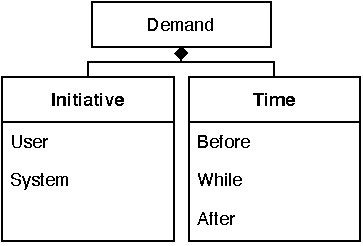
\includegraphics{contents/05_model_description/res/model_demand_overview.pdf}
    \end{center}
    \caption{Übersicht über den \textit{Demand} für Erklärungen}
    \label{fig:model_demand_overview}
\end{figure}

\subsubsection{Bedarf}

Der \textit{Demand}  für Erklärungen kann aus verschiedenen Perspektiven betrachtet werden. Bei welcher Aufgabe und bei welchen Ereignissen Erklärungen überhaupt benötigt werden, muss in den Anforderungen für Erklärungen festgehalten werden. Diese entstehen auf Basis der \textit{External Dependencies}. Unter der Kategorie \textit{Demand} in diesem Modell ist zusätzlich festgehalten, auf welche Initiative hin (\textit{Initiative}) und zu welchem Zeitpunkt in Bezug auf ein Ereignis im System dem \textit{End User} Erklärungen vom System zur Verfügung gestellt werden sollen. Einen Überblick über die Verwendung verschiedener Ausprägungen der Aspekte ist in \autoref{fig:model_demand_overview} und \autoref{tab:explanation_demands} dargestellt.

\begin{table}[bht!]
    \begin{center}
        \begin{tabular}{p{.25\textwidth}p{.25\textwidth}p{.41\textwidth}}
            \hline
            Aspekt    & Ausprägung   & Quellen \\
            \toprule
            Initiative  &  Manual       & \cite{chazette_end-users_nodate} \cite{tintarev_designing_nodate}
                                            \cite{wiegand_id_2020} \\
                        &  Automatic    & \cite{chazette_end-users_nodate} \cite{eiband_impact_2019}
                                            \cite{wiegand_id_2020} \cite{schaffer_i_2019}
                                            \cite{yamada_evaluating_2016} \\
            \tablerowspacing
            Time        &  Before       & \cite{rosenfeld_explainability_2019} \cite{wiegand_id_2020}
                                            \cite{kunkel_let_2019} \cite{koo_why_2015} \cite{haspiel_explanations_2018} 
                                            \cite{haspiel_explanations_2018} \\
                        &  while        & \cite{rosenfeld_explainability_2019} \cite{wiegand_id_2020}
                                            \cite{kunkel_let_2019} \\
                        &  After        & \cite{rosenfeld_explainability_2019} \cite{wiegand_id_2020}
                                            \cite{kunkel_let_2019} \cite{koo_why_2015} \cite{haspiel_explanations_2018}
                                            \cite{wiegand2019drive} \cite{haspiel_explanations_2018} \\
            \toprule
        \end{tabular}
    \end{center}
    \caption{Der Bedarf einer Erklärung zusammen mit in der Literatur untersuchten Einflüssen auf die Qualität von Erklärungen}
    \label{tab:explanation_demands}
\end{table}

\paragraph{Initiative} Die \textit{Initiative} einer Erklärung ist der Auslöser für das Geben von Erklärungen in einem System. Eine Möglichkeit ist eine automatische Auslieferung der Erklärung an den \textit{End User}. Das System trifft dann allein die Entscheidung, wann und ob \textit{End User} eine Erklärung bekommt (\textit{Automatic}). Alternativ können Erklärungen vom \textit{End User} manuell angefordert werden (\textit{Manual}).

\paragraph{Time} Die \textit{Time} ist der Zeitpunkt im Verhältnis zu einem Ereignis, zu dem das System eine Erklärung bereitstellt. \citeauthor{rosenfeld_explainability_2019} sowie \citeauthor{wiegand_id_2020} haben explizit untersucht, wann Erklärungen angezeigt werden sollten, wenn ein Ereignis im System auftritt oder das System eine Aktion durchführt. Dies umfasst die Möglichkeiten vor dem Ereignis (\textit{Before}), während (\textit{While}) oder nach dem Ereignis (\textit{After}) eine Erklärung zu diesem zu liefern \cite{rosenfeld_explainability_2019, wiegand_id_2020}. Letzteres wird in der Literatur zum Teil auch als \textit{Posthoc-Explanation} referenziert \cite{sokol_explainability_2020}.

\smallskip

Im Rahmen von \textbf{RQ2} kann an dieser Stelle der \textit{Demand} als relevante Eigenschaft von Erklärungen für die Erklärungsqualität festgehalten werden.

\begin{figure}[htb!]
    \begin{center}
        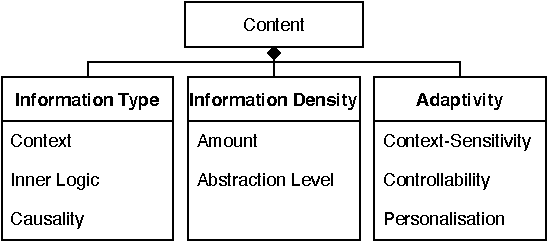
\includegraphics{contents/05_model_description/res/model_content_overview.pdf}
    \end{center}
    \caption{Übersicht über den \textit{Content} von Erklärungen}
    \label{fig:model_content_overview}
\end{figure}

\subsubsection{Inhalt}

Unter dem Punkt \textit{Content} wird definiert, mit welchen Inhalten die \textit{End User} durch Erklärungen versorgt werden \cite{nunes_systematic_2017}. Dieser ist einer von zwei Teilen des Modells, welcher sich auf die Granularität von Erklärungen bezieht. Der \textit{Content} beinhaltet nicht nur den Informationstyp (\textit{Information Type}) den das System vermittelt, sondern auch wie viel Inhalt (\textit{Information Density}). Ein weiterer Aspekt ist Anpassungsfähigkeit der Inhalte (\textit{Adaptivity}). \autoref{tab:content_of_explanations} und \autoref{fig:model_content_overview} enthalten die verschiedenen Ausprägungen dieser Aspekte zusammen mit deren Anwendungen in der Literatur, welche einen Einfluss auf die externe Qualität von Erklärungen haben.

\begin{table}[bht!]
    \begin{center}
        \begin{tabular}{p{.25\textwidth}p{.25\textwidth}p{.41\textwidth}}
            \hline
            Aspekt    & Ausprägung   & Quellen \\
            \toprule
            Information Type        & Context     & \cite{chazette2020explainability} \cite{zahedi_towards_2019}
                                                \cite{cassens_ambient_2019} \cite{zahedi_towards_2019}
                                                \cite{zolotas_towards_2019} \cite{chari_explanation_2020}
                                                \cite{nunes_systematic_2017} \cite{ribera2019can} \\
                            & Inner Logic & \cite{chazette2020explainability} \cite{sato_action-triggering_2019} 
                                                \cite{thomson_knowledge--information_2020}
                                                \cite{chari_explanation_2020} \cite{neerincx_using_2018}
                                                \cite{ribera2019can} \cite{cassens_ambient_2019} \\
                                & Causality &   \cite{chazette2020explainability} \cite{abdulrahman_belief-based_2019}
                                                \cite{yamada_evaluating_2016} \cite{sato_action-triggering_2019}
                                                \cite{zahedi_towards_2019} \cite{zahedi_towards_2019}
                                                \cite{zolotas_towards_2019} \cite{cassens_ambient_2019}
                                                \cite{thomson_knowledge--information_2020}
                                                \cite{chari_explanation_2020} \cite{neerincx_using_2018}
                                                \cite{nunes_systematic_2017}\cite{zhu_effects_2020}
                                                \cite{ribera2019can} \cite{lim_2009_assessing} 
                                                \cite{kaptein_personalised_2017} \\
            \tablerowspacing
            Information          & Amount &      \cite{ribera2019can} \cite{kouki_user_2017}
                                                \cite{hernandez-bocanegra_effects_2020} \cite{martin_developing_2019} \\
            Density              & Abstraction Level & \cite{thomson_knowledge--information_2020}
                                                \cite{hernandez-bocanegra_effects_2020} \\
            \tablerowspacing
            Adaptivity          & Context-Sensitivity & \cite{kaptein_personalised_2017} \cite{cassens_ambient_2019} \\
                                & Controllability & \cite{abdulrahman_belief-based_2019} \cite{cheng2019explaining} \\
                                & Personalization & \cite{kaptein_personalised_2017} \cite{cassens_ambient_2019}
                                                    \cite{sokol_one_2020} \cite{tintarev_designing_nodate}
                                                    \cite{sokol_explainability_2020} \\
            \toprule
        \end{tabular}
    \end{center}
    \caption{Eigenschaften einer Erklärung bezogen auf den Inhalt einer Erklärung mit in der Literatur gezeigtem Einfluss auf die externe Qualität von Erklärungen}
    \label{tab:content_of_explanations}
\end{table}

\paragraph{Information Type} Der \textit{Information Type} beschreibt die Inhalte, die \textit{End Usern} mithilfe der Erklärung übermittelt werden. Unter diesem Aspekt sind in der Literatur sehr verschiedene Ansätze zu finden, die unterschiedliche Typen definieren. Beispielsweise stellen \citeauthor{chazette_end-users_nodate} mithilfe von Fragewörtern verschiedene Informationstypen dar \cite{chazette_end-users_nodate}, während \citeauthor{rosenfeld_explainability_2019} selbige Fragewörter nutzt, um andere Inhalte zu beschreiben und weitere ergänzt. Grundsätzlich kann zwischen globalen Erklärungen, die immer gültig sind und situationsabhängigen (lokalen) Erklärungen unterschieden werden \cite{lim_2009_assessing}. Zusammen mit weiteren Arbeiten \cite{kaptein_personalised_2017, abdulrahman_belief-based_2019} wurden die verschiedenen Definitionen in drei verschiedene Informationstypen gebündelt. Diese fassen die in der Literatur am häufigsten transportierten Informationen zusammen. Allerdings bilden die drei Ausprägungen nicht alle möglichen Informationen in Erklärungen ab.

Kontextinformationen in einer Erklärung geben Auskunft über die zugrundeliegenden Daten (\textit{Context}). Dabei werden die eingehenden Informationen auf Basis derer das System Entscheidungen trifft, dem \textit{End User} dargelegt.

Eine weitere Möglichkeit ist das Erklären der Funktionsweise von Algorithmen eines Systems (\textit{Inner Logic}). Dies sind die Informationen, wie genau ein System die ihm zur Verfügung stehenden Daten verarbeitet und interpretiert.

Ein dritter Weg ist die Erklärung von Zusammenhängen zwischen den Eingaben und Ausgaben des Systems (\textit{Causality}). In einer solchen Erklärung wird den \textit{End Usern} der Grund für ein bestimmtes Systemverhalten oder eine Entscheidung erklärt. Hierbei gibt es verschiedene Optionen, Gründe zu erläutern. Eine Erklärung dieser Art kann die Information enthalten, warum ein bestimmtes Systemverhalten in einer Situation erfolgt ist. Auch kann eine Erklärung vermitteln, warum ein alternatives Verhalten oder eine alternative Ausgabe des Systems nicht erfolgt ist \cite{martin_evaluating_2021}.

\paragraph{Information Density} Die \textit{Information Density} beschreibt die Menge und die Kompaktheit an Informationen, die eine Erklärung enthält. Dabei ist einerseits wichtig, ob \textit{End Usern} alle vorliegenden Erklärungsmöglichkeiten vom System angezeigt werden (\textit{Amount}). Andererseits spielt es eine Rolle mit welchem Detailgrad die Informationen dargestellt werden (\textit{Abstraction Level}). Zum Beispiel können \textit{End Usern} wenig Informationen angezeigt werden, die nicht die vollen Details abdecken, um diese nicht zu überfordern.

\paragraph{Adaptivity} \textit{Adaptivity} definiert, wie statisch die Erklärungen in einem System sind. Eine Ausprägung ist dabei der Grad, zu dem eine Erklärung auf den aktuellen \textit{Context} angepasst ist (\textit{Context-Sensitivity}). Außerdem beinhaltet \textit{Adaptivity} die \textit{Personalisation}, welche darstellt, inwiefern Erklärungen auf den aktuellen \textit{End User} anpassbar sind, zum Beispiel an dessen Expertise. \textit{Controllability} beschreibt dabei, welchen Einfluss \textit{End User} haben, mit der Erklärung zu interagieren. Unter diesen Aspekt fällt unter anderem die Möglichkeit, dass \textit{End User} Erklärungen optional anfordern können oder sie innerhalb eines Erklärungsdialogs navigieren können.

\bigskip

An dieser Stelle kann für \textbf{RQ2} hinzugefügt werden, dass auch der \textit{Content} einer Erklärung einen großen Einfluss auf die externe Qualität von Erklärungen hat. Dies lässt sich unter anderem an der Anzahl an Autoren festmachen, die verschiedene Facetten des Einflusses durch den \textit{Content} von Erklärungen auf die Qualität untersuchen.

\subsubsection{Presentation}

Nachdem nun sowohl der \textit{Demand} als auch der an den \textit{End User} übermittelte Inhalt als zentrale \textit{Characteristics} von Erklärungen vorgestellt wurden, fehlt im Modell die Art der Präsentation der Erklärung an den \textit{End User}. Diese ist mit ihren zugehörigen Ausprägungen unter \textit{Presentation} zusammengefasst (siehe \autoref{fig:model_presentation_overview}). Sie stellt den zweiten Teil der Granularität von Erklärungen dar. Zu dem Aspekt gehören in diesem Modell für Erklärungen das Medium (\textit{Medium}), über das die Erklärung \textit{End Usern} bereitgestellt wird, der verwendete Ton (\textit{Tone}) des \textit{Explainers} (siehe \autoref{02_basics:explainability}) \cite[vgl.][]{chazette_knowledge_nodate} und die Gruppierung von Erklärungen respektive Erklärungstypen (\textit{Grouping}). \autoref{tab:presentation_of_explanations} stellt die Ausprägungen zusammen mit der Literatur, die den entsprechenden Aspekt in Bezug auf die externe Qualität von Erklärungen untersucht, dar.

\begin{figure}[t!]
    \begin{center}
        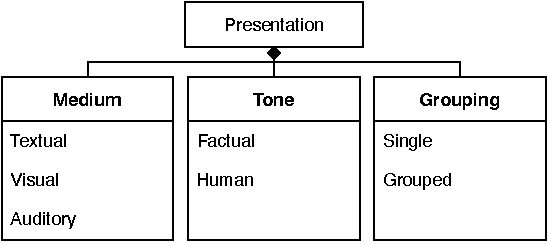
\includegraphics{contents/05_model_description/res/model_presentation_overview.pdf}
    \end{center}
    \caption{Übersicht über die \textit{Presentation} von Erklärungen}
    \label{fig:model_presentation_overview}
\end{figure}

\paragraph{Medium} Das \textit{Medium} einer Erklärung ist der Informationsträger für die \textit{Presentation} der Inhalte. Dabei können verschiedene Möglichkeiten aus dem Multimedia-Bereich verwendet werden. In der Literatur untersucht wurden Texterklärungen (\textit{Textual}), visuelle Darstellungen wie z.~B. Diagramme (\textit{Visual}) sowie auditive Erklärungen (\textit{Auditory}). Insbesondere dieser Aspekt bietet Möglichkeiten für Mischformen und Kombinationen \cite{kouki_user_2017}.

\paragraph{Tone} Der \textit{Tone} einer Erklärung bestimmt die Art, wie \textit{End Usern} der Inhalt einer Erklärung näher gebracht wird. Das Spektrum der Möglichkeiten erstreckt sich dabei vor allem zwischen sehr faktisch gehaltenen Erklärungen (\textit{Factual}) und persönlichen bzw. menschlichen Erklärungen (\textit{Human}). Ein Beispiel wäre die Bereitstellung von Erklärungen über einen persönlichen Assistenten \cite{schaffer_i_2019}.

\paragraph{Grouping} Mit dem \textit{Grouping} von Erklärungen wird bestimmt, wie viele Erklärungen \textit{End Usern} gleichzeitig beziehungsweise kombiniert präsentiert werden. Zum Beispiel können erklärende Grafiken wie Graphen mit Texterklärungen kombiniert werden. Grundsätzlich gibt es dabei die Möglichkeiten eine Erklärung zu einem Zeitpunkt anzuzeigen (\textit{Single}) oder mehrere Erklärungen bzw. Erklärungstypen zu gruppieren (\textit{Grouped}). Bei letzterem können entweder Erklärungen mit verschiedener \textit{Presentation} aber dem gleichen \textit{Content} kombiniert werden \cite{kouki_user_2017} oder mehrere einzelne Erklärungen zusammen dargestellt werden \cite{balog_measuring_2020}.

\bigskip

Als letzter Teil der Antwort auf \textbf{RQ2} kann die \textit{Presentation} mit den dazugehörigen Aspekten als Eigenschaft von Erklärungen mit einem Einfluss auf die externe Qualität von Erklärungen ergänzt werden.

\newpage

\begin{table}[htb!]
    \begin{center}
        \begin{tabular}{p{.25\textwidth}p{.25\textwidth}p{.41\textwidth}}
            \hline
            Aspekt     & Ausprägung & Quellen \\
            \toprule
            Medium              & Textual  &    \cite{sokol_explainability_2020} \cite{balog_measuring_2020}
                                                \cite{tintarev_designing_nodate} \cite{sato_action-triggering_2019}
                                                \cite{eiband_impact_2019} \cite{eiband_impact_2019}
                                                \cite{abdulrahman_belief-based_2019} \cite{cassens_ambient_2019}
                                                \cite{nunes_systematic_2017} \\
                                & Visual    &   \cite{sokol_explainability_2020} \cite{sato_action-triggering_2019} 
                                                \cite{mucha_interfaces_2021} \cite{abdulrahman_belief-based_2019}
                                                \cite{nunes_systematic_2017} \cite{schrills_color_2020} \\
                                & Auditory     &   \cite{wiegand2019drive} \cite{nunes_systematic_2017}
                                                \cite{wang_is_2018} \\
            \tablerowspacing
            Tone                & Factual   &   \cite{eiband_impact_2019} \cite{abdulrahman_belief-based_2019}
                                                \cite{kunkel_let_2019} \cite{neerincx_using_2018} \\
                                & Human     &   \cite{abdulrahman_belief-based_2019} \cite{kunkel_let_2019}
                                                \cite{weitz_you_2019} \cite{zahedi_towards_2019}
                                                \cite{neerincx_using_2018} \\
            \tablerowspacing
            Grouping            & Single    &   \cite{nunes_systematic_2017} \cite{balog_measuring_2020}
                                                \cite{sato_action-triggering_2019} \cite{eiband_impact_2019}
                                                \cite{abdulrahman_belief-based_2019} \\
                                & Grouped   &   \cite{nunes_systematic_2017} \cite{balog_measuring_2020}
                                                \cite{tintarev_designing_nodate}  \\
            \toprule
        \end{tabular}
    \end{center}
    \caption{Verschiedene Übermittlungsmöglichkeiten für Erklärungen an den \textit{End User}, die in der Literatur einen Effekt auf die externe Qualität von Erklärungen gezeigt haben}
    \label{tab:presentation_of_explanations}
\end{table}

\noindent\fbox{
    \parbox{0.964\textwidth}{
        \smallskip
        \textbf{RQ2} Welche Eigenschaften von Erklärungen haben einen Einfluss auf die externe Qualität eines erklärbaren Systems?
        \smallskip
    }
}

\smallskip

Der in diesem Abschnitt vorgestellte Teil des Modells für Erklärungen (\textit{Characteristics}) beinhaltet die Antwort auf die zweite Forschungsfrage. Dabei sind explizit die Eigenschaften \textit{Demand}, \textit{Content} und \textit{Presentation} mit einem Einfluss auf die externe Qualität von Erklärungen zu benennen. Die genauen Ausprägungen dieser Eigenschaften werden als Unterpunkte der jeweiligen Aspekte im Modell enthalten. Die Ergebnisse, die in dem Modell zusammengefasst sind, entspringen dabei der Evaluation von Erklärungen mit verschiedenen Eigenschaften in der Literatur.

\subsection{Evaluation}
\label{sec:model_evaluation_description}

Die Metriken und die Vorgehensweise, die für die \textit{Evaluation} ausgewählt wird, hängt folglich sehr eng mit den zuvor festgelegten \textit{Objectives} zusammen.

\paragraph{Target} Zunächst muss bei der Evaluation geklärt werden, was der Prüfgegenstand ist. Dabei gibt es vor allem zwei große Möglichkeiten im Kontext der Erklärbarkeit. Entweder werden die integrierten Erklärungen an sich evaluiert und die Studienteilnehmer darauf explizit angesprochen oder es werden die Auswirkungen auf verschiedene System-Metriken ausgewertet. Auch eine Kombination ist möglich.

\paragraph{Strategy} Beim Festlegen der \textit{Strategy} der Evaluation gibt es verschiedene Möglichkeiten, die unter anderem vom \textit{Context} abhängen. Je nachdem, welche Ergebnisse die Stakeholder, die Erklärungen in ein System integrieren möchten, benötigen, muss die Evaluation kontrollierter oder weniger kontrolliert sein \cite[vgl.][]{wohlin2012experimentation}.

\paragraph{Metrics} \textit{Metrics} sind klar definierte Messungen, die durchgeführt werden, um die zuvor festglegten \textit{Objectives} zu überprüfen.

Die Literaturrecherche hat wie bereits \cite{nunes_systematic_2017} nur empirische Studien zur Evaluation von Erklärungen gefunden.

Entsprechend \cite{wohlin2012experimentation} habe ich die verschiedenen Evaluationsmethoden in \textit{Qualitaative Research} und \textit{Quantitative Research} gegliedert.

\begin{table}[htb!]
    \begin{center}
        \begin{tabular}{|p{.3\textwidth}|p{.3\textwidth}|p{.3\textwidth}|}
            \hline
            \textbf{Evaluationstyp} & \textbf{Empirische Strategie} & \textbf{Quellen} \\ \hline
            Qualitativ  & Subjective Perception Questionaire &  \cite{balog_measuring_2020} \cite{sato_context_nodate}
                                                                \cite{waa_evaluating_2021} \cite{eiband_impact_2019}  \cite{kouki_user_2017} \cite{tsai_evaluating_2019}
                                                                \cite{hernandez-bocanegra_effects_2020}
                                                                \cite{zahedi_towards_2019} \cite{tsai_effects_2020} 
                                                                \cite{ribera2019can} \\
                        & Acceptance                        & \cite{tintarev_designing_nodate}
                                                            \cite{hernandez-bocanegra_effects_2020}
                                                            \cite{kunkel_let_2019} \\
                        & Think aloud                       & \cite{wiegand_id_2020} \cite{yamada_evaluating_2016} \\
                        & Preference                        & \cite{kouki_user_2017} \cite{mucha_interfaces_2021} 
                                                            \cite{abdulrahman_belief-based_2019} 
                                                            \cite{waa_evaluating_2021} \cite{wiegand_id_2020} ,
                                                            \cite{stange_effects_2021} \cite{kaptein_personalised_2017} \\
                        & Mental Model Understanding        & \cite{gunning2019darpa} \\
                        & Cognitive Workload                & \cite{wiegand2019drive, wiegand_id_2020} \\
            \hline
            Quantitative& Explanation exposure delta & \\
                        & Accuracy                          & \cite{tintarev_designing_nodate}
                                                            \cite{waa_evaluating_2021} \cite{mucha_interfaces_2021}
                                                            \cite{kunkel_let_2019} \cite{zolotas_towards_2019} \\
                        & Learning Rate                     & \cite{tintarev_designing_nodate} \cite{gunning2019darpa} \\
                        & Task Performance                  & \cite{waa_evaluating_2021}  \cite{mucha_interfaces_2021}  
                                                            \cite{abdulrahman_belief-based_2019} 
                                                            \cite{zolotas_towards_2019} \cite{martin_developing_2019} 
                                                            \cite{martin_evaluating_2021} \cite{gunning2019darpa} \\
            \hline
        \end{tabular}
    \end{center}
    \caption{Evaluation}
    \label{tab:evaluation_of_explanations}
\end{table}


Laut \cite{balog_measuring_2020} sind die 8 verschiedenen Ziele korreliert und müssen nicht einzeln gemessen werden. Hoch korreliert \cite{kouki_user_2017}

Cognitive Workload 

Einen vollständigen Überblick über die Qualität einer Erklärung bekommt man, wenn man Satisfaction, Scrutability und Translarency misst \cite{balog_measuring_2020}.

\glqq Importantly however, such measures often only measure one aspect of behavior. Ideally, a combination of both measurement types should be used to assess effects on both the user’s perception and behavior. In this way, a complete perspective on a construct can be obtained.\grqq{} (Qualitative / Quantitavie) \cite{waa_evaluating_2021}

Number of detailed looks

\subsubsection{Example Questions for questionaires}

NASA-TLX \cite{tsai_evaluating_2019}

Effectiveness helps me to determine how well I will like this movie does not help me make a decision about this item Efficiency helps me to decide faster if I will like this movie does not save me time Persuasiveness makes me want to watch this movie fails to make this item appeal to me Satisfaction would improve how easy it is to pick a recommendation does not satisfy me Scrutability would allow me to give feedback on how well my preferences have been understood would make it difficult for me to correct the reasoning behind the recommendation Transparency helps me to understand what the recommendation is based on fails to reveal the reasoning behind this recommendation Trust helps me to trust the recommendation does not seem credible \cite{balog_measuring_2020}

\cite{knijnenburg2012explaining, hernandez-bocanegra_effects_2020} have something for exact evaluation of overall explanation quality

\cite{weitz_you_2019} trusted automation questionaire

Directly based on the explatnation \cite{sato_action-triggering_2019} or other metrics 

DARPA (used by \cite{martin_evaluating_2021}) \cite{gunning2019darpa}

Domain specifc metrics. For example for explainable AI (Predictive systems) TYN (Trust-Your-Neighbours) or Meet in the Mittle (MITM) \cite{martin_evaluating_2021}

Questions for quality factors:

\subsubsection{Direkte Metriken}

Bei der direkten Messung der Qualität von Erklärungen werden in der Literatur ledig verschiedene Möglichkeiten zur subjektiven Evaluation vorgestellt.

Neben den in \autoref{sec:model_external_dependencies} vorgestellten Qualitätsaspekten, die als Qualitätsziele für die Integration von Erklärungen definiert definiert wurden, gibt es weitere Aspekte, die in der Literatur zur Messung der Qualität von Erklärungen vorgestellt wurden \cite[sato_action-triggering_2019, ], die im folgenden erläutert werden.

\paragraph{Usefulness}

\paragraph{Completeness}

\paragraph{Correctness}

Bei der Messung der direkten Messung der Erklärugnsqualität setzt die Literatur vor allem Likert-Skalen ein. Dabei handelt es sich um einen Ordinalskala mit in der Regel fünf oder sieben einzelnen Bewertungsschritten, auf denen einen Aussage bewertet wird. Die genaue Benennung der Bewertungsschritte erfolgt in der Literatur verschieden. Allerdings werden durchweg solche mit einer inhaltlichen Übereinstimmtung zu \glqq Volle Zustimmung\grqq{}, \glqq Teilweise Zustimmung\grqq{}, \glqq Neutral\grqq{},\glqq Teilweise Ablehnung\grqq{} und \glqq Volle Ablehnung\grqq{} verwendet \cite{sato_action-triggering_2019, sato_context_nodate, wang_is_2018, hoffman_metrics_nodate}. \autoref{tab:evaluation_direct_measures_evaluation} stellt eine Übersicht von verwendeten Aussagen für die Messung der verschiedenen Aspekte dar. Aufgelistet sind nur verallgemeinerbare Aussagen und nicht einen spezifischen \textit{Context} betreffende Aussagen. In spitzen Klammer sind Platzhalter dargestellt, um die aufgelisteten Aussagen auf den eigenen \textit{Context} anzupassen.

\begin{table}
    \begin{center}
        \begin{tabular}{|p{0.25\textwidth} p{0.5\textwidth} p{0.15\textwidth}|}
            \hline
            \textbf{Qualitätsaspekt} & \textbf{Aussage} & \textbf{Quellen} \\
            \hline
            \hline
            Transparency    & & \\
            \hline
            Satisfaction    & Ich bin zufrieden mit der Erklärung, um zu verstehen, warum das System seine Entscheidung 
                                getroffen hat.
                                & \cite[vgl.][]{riveiro_thats_2021} \\
            \hline
            Transparency    & & \\
            \hline
            Persuasiveness  & Die Erklärung ist überzeugend.
                                & \cite[vgl.][]{sato_action-triggering_2019, sato_context_nodate} \\
                            & Die Erklärung weckt Interesse. 
                                & \cite[vgl.][]{sato_action-triggering_2019, sato_context_nodate} \\
            \hline
            Usefulness      & Die Erklärung ist einfach zu verstehen. 
                                & \cite[vgl.][]{sato_action-triggering_2019, sato_context_nodate} \\
                            & Die Erklärung ist nützlich bei der Erfüllung von <Aufgabe>.
                                & \cite[vgl.][]{sato_action-triggering_2019, sato_context_nodate} \\
            \hline
            Completeness    & & \\
            \hline
            Completeness    & & \\
            \hline
        \end{tabular}
    \end{center}
    \caption{}
    \label{tab:evaluation_direct_measures_evaluation}
\end{table}

\subsubsection{Indirekte Metriken}

\begin{itemize}
    \item Satisfaction: The explanations provided of how the AI-system classifies text are satisfying. \cite{riveiro_thats_2021}
    \item Completeness: The explanations provided regarding how the AI-system classifies the text seem complete
 \cite{riveiro_thats_2021}
    \item Completeness: Would you have liked for the explanations to contain additional information? If so, what type of information and when, i.e., in which situations?
 \cite{riveiro_thats_2021}
    \item Sufficient detail: The explanations provided of how the AI-system works have sufficient detail.
 \cite{riveiro_thats_2021}
    \item Understanding: From the explanations provided, I understand how the AI-system works.
 \cite{riveiro_thats_2021}
 \item Transparency: I understand the robot’s decision-making process \cite{wang_is_2018}
 \item Understandability: The explanation helps me understand how the [software, algorithm, tool] works. \cite{hoffman_metrics_nodate}
 \item Satisfaction: The explanation of how the [software, algorithm, tool] works is satisfying. \cite{hoffman_metrics_nodate}
 \item Completeness: The explanation of how the [software, algorithm, tool] works is sufficiently complete. \cite{hoffman_metrics_nodate}
 \item Helpfull: The explanation is actionable, that is, it helps me know how to use the [software, algorithm, tool] \cite{hoffman_metrics_nodate}
 \item Correctness: The explanation lets me know how accurate or reliable the [software, algorithm] is.\cite{hoffman_metrics_nodate}
 \item Trust: The explanation lets me know how trustworthy the [software, algorithm, tool] is. \cite{hoffman_metrics_nodate}
\end{itemize}


Tabelle der Metriken nach \cite{carvalho2017quality} (Ubiqutous Systems)

Trustworthiness: \cite{schrills_color_2020}

(FOST Scale: Facets of System Trustworthiness)
Please indicate to what extent you agree with the following statements 01 The system’s classification is reliable 02 The system’s classification is precise 03 The system’s classification is traceable 04 I can trust the system’s classification 05r I cannot depend on the system’s classification 06 With the help of the visualization I am able to identify wrong mechanisms of the AI 07 I agree with the classification 08 The visualization provides a good explanation for the classification

\cite{tintarev_designing_nodate} haben Messliste gebaut.

(Task performance) \cite{martin_evaluating_2021}

Qualität von Erklärungen zu bestimmen ist nicht einfach.

\cite{tsai_effects_2020}:

Construct E: Perceived System Effectiveness • E1: Using the system is a pleasant experience. • E2: I made better choices with the recommender. • E3: I found better items using the recommender. • E4: I felt bored when using the recommender. • Construct T: Perceived Trust • T1: I am convinced by the scholar recommended to me. • T2: I am confident I will like the items recommended to me. • T3: The recommender made me more confident about my selection/decision. • T4: The recommender can be trusted. • Construct P: Perceived Transparency • P1: The provided information was sufficient for me to make a good decision. • P2: The recommender explained why the scholars were recommended to me. • P3: I understood why the scholars were recommended to me. • Construct S: Satisfaction • S1: I will use this recommender again. • S2: I will tell my friends about this recommender. S3: Overall, I am satisfied with the recommender. • S4: The recommender helped me find the ideal contacts at the conference.

Special measures like ICM for ML-Models which is tied to the input and output of the model \cite{waa_evaluating_2021, neerincx_using_2018}

Trust questions: originally by \cite{mayer1999effect} used by \cite{wang_is_2018}

Specific trust items e.g. for human-robot interaction used by \cite{zhu_effects_2020} originally developed by \cite{schaefer2013perception}

Just different Begriffe mit Likert SCale (Satisfaction / Trust / Transparency) \cite{koo_understanding_2016, koo_why_2015} Behavioral is again domain specific

3 Types of Evaluation according to \cite{ribera2019can, doshi2017towards}: (1) applicationgrounded evaluation with real humans and real tasks; (2) human-grounded evaluation with real humans but simplified tasks; and (3) functionally-grounded evaluation without humans and proxy tasks; all of them always inspired by real tasks and real humans’ observations.

 \cite{tintarev2007survey}:
 
 Transparency: Qualitytive: Does the User understand the system Quantitative: correctness, completion time
 
 Scrutability: Hard to measure due to many confoundings
 
 Trust: Questionaires, Loyalty: Number of Logins, usesages (S. M. McNee, S. K. Lam, J. A. Konstan, and J. Riedl. Interfaces for eliciting new user preferences in recommender systems. User Modeling, pages pp. 178–187, 2003.)
 
 Persuasiveness: Questionaires + Domain-Specific Performance metrics
 
 Effectiveness: accuracy measures (Domain-Specific) 
 
 Efficiency: Task completion time, Number of times an explanation is called
 
 Satisfaction: User preference (Differentiate explanation and system), number of usability problems
 
 Wichtig ist auch das Messen von anderen Qualitätsaspekten, die nicht 

\newpage

\begin{figure}[htb!]
    \begin{center}
        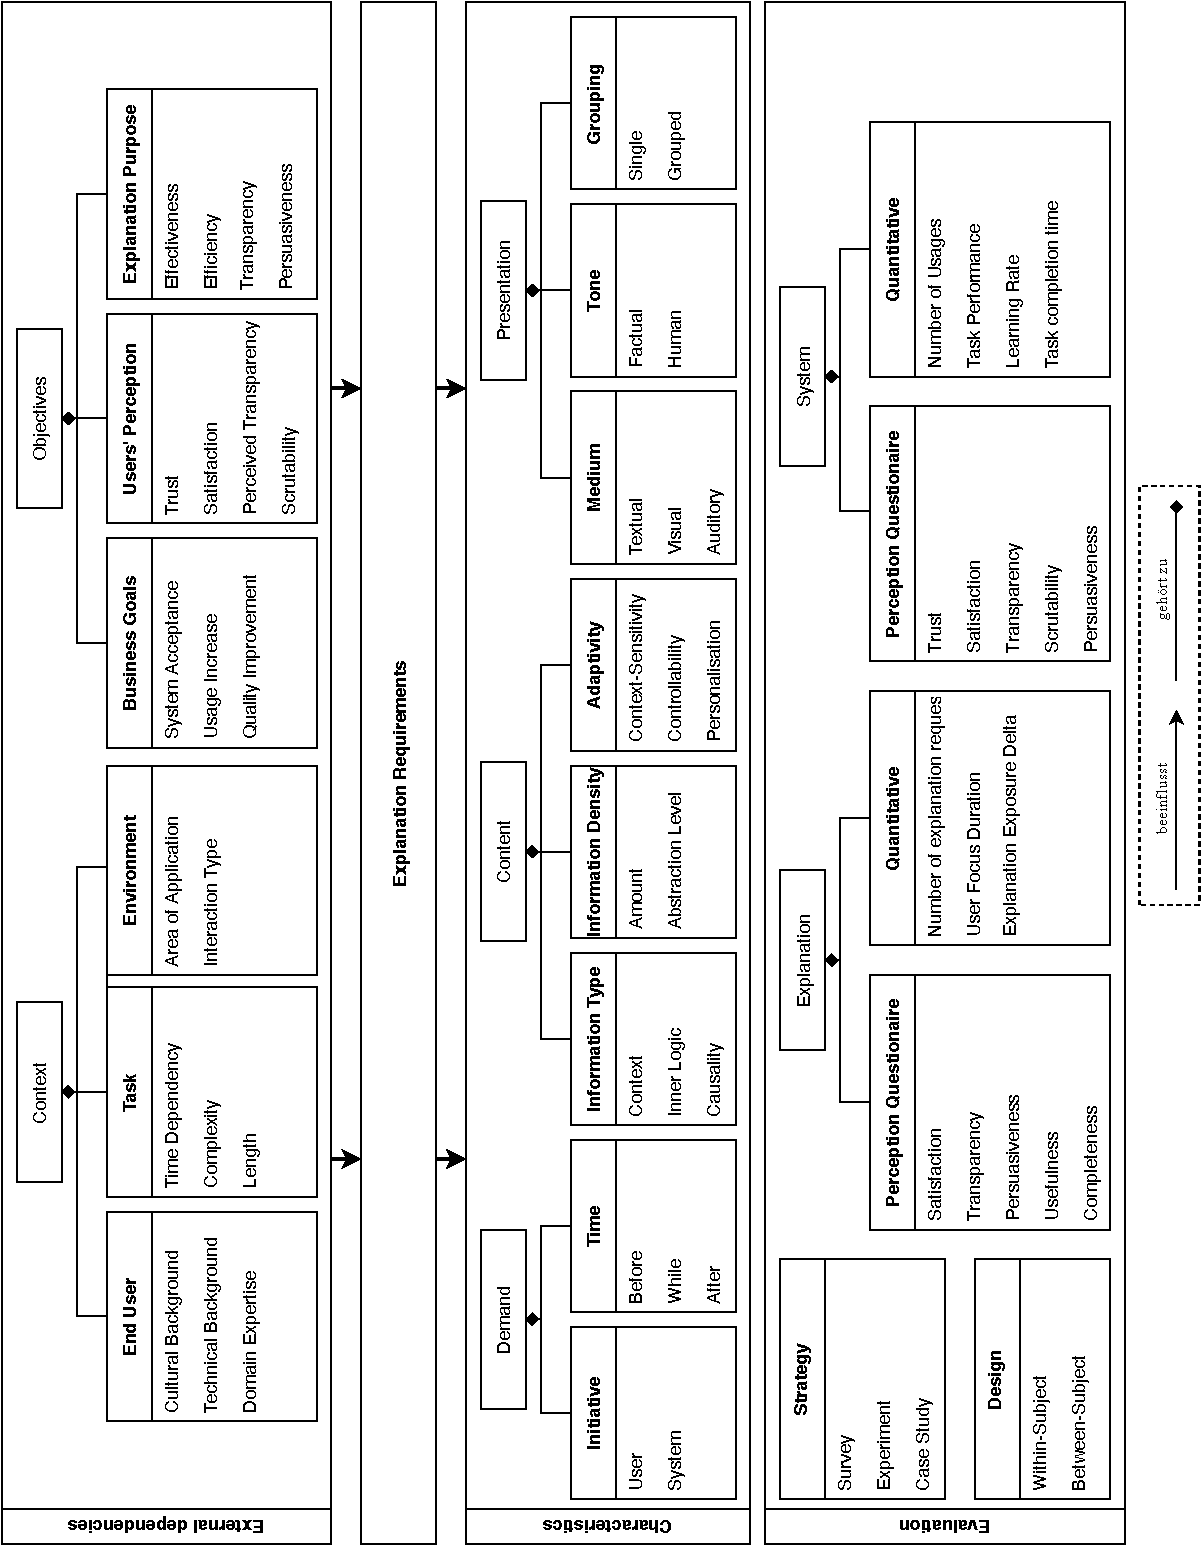
\includegraphics[width=\textwidth]{contents/05_model_description/res/model_overview_complete.pdf}
    \end{center}
    \caption{Übersicht über die Aspekte von Erklärbarkeit sowie dessen bekannte Ausprägungen aus der Literatur}
    \label{fig:model_overview_complete}
\end{figure}

\newpage

\section{Abhängigkeiten}
\label{sec:model_proved_relations}

\cite{international2011iso} definiert ein Konzept, um Zusammenhänge zwischen Charakteristiken eines Systems und Qualitätsaspekten zu definieren. Anwendung findet dies unter Anderem bei \cite{carvalho2020developers}. Das Konzept beschreibt, dass einzelne Eigenschaften von Softwaresystemen einen positiven (\textcolor{green}{helps}), negativen (\textcolor{red}{hurts}) oder neutralen Effekt auf Qualitätsaspekte haben kann. Diese können entweder generell gelten oder unter bestimmten Bedingungen (Kontexten) zutreffen.

\subsection*{Demand}

\subsubsection*{Positiv}

Eine Erklärung die den Kontext des Systemverhaltens wiederspiegelt wirkt sich positiv auf die Persuasiveness und die Usefullness einer Erklärung aus. Bewiesen ist dies nur für Recommender Systeme \cite{sato_action-triggering_2019, abdulrahman_belief-based_2019}

Eine Erklärung, die darstellt, warum eine Alternative nicht genommen wurde, wird besser verstanden als eine, welche die aktuelle Entscheidung erklärt. \cite{schrills_color_2020}

(2) Rational explanations are only effective on users that report being very unfamiliar with a task – regardless of their actual competency level. \cite{schaffer_i_2019}

Das proaktive Präsentieren von Erklärungen, wenn diese einen geringen Inhalt haben wirkt sich positiv auf die Usability aus.

Das Anzeigen von Erklärungen vor einem Event hat einen positiveren Einfluss auf Trust als das Anzeigen danach. \cite{haspiel_explanations_2018}

Proaktive Erklärungen in unvorhersehbaren Situation, erhöhen das Vertrauen \cite{zhu_effects_2020}

Das anzeigen von Erklärungen bei sicherheitsrelevanten Systemfunktionen hat einen positiven Einfluss auf satisfaction und trust. \cite{wiegand2019drive}

Nutzer wollen immer Zugriffsmöglichkeiten auf erklärungen \cite{chazette_end-users_nodate}

\subsubsection*{Negativ}

(3) There is a danger in showing explanations to self-confident users in that situation awareness might be negatively impacted – this can be mitigated by requiring interaction with an agent. \cite{schaffer_i_2019}

\subsubsection*{Beides}

Der Zusammenhang zwischen dem Grad der Systembeeinflussung durch den Nutzer und dem Erklärungsbedarf ist antiproportional. Umso mehr mehr Kontrolle der Nutzer über ein System erhält, umso weniger Erklärungsbedarf hat dieser \cite{rosenfeld_explainability_2019}.

Wenn der Nutzer generell ein hohes Vertrauen in ein System hat, dann benötigt dieser keine Erklärungen, um dieses herzustellen. \cite{rosenfeld_explainability_2019, doshi2017towards}

Die User Satisfaction kann leiden, wenn die Nutzer das System bereits gut kennen, wenn eine Erklärung angezeigt wird.

\subsection*{Granularität}

\subsubsection*{Positiv}

Hybride Stile (Typ + Inhalt) haben den größten positiven Einfluss auf die Usability und Persuasiveness eines Recommender Systems im Gegensatz zu einzeln ausgewählten Stilen. \cite{sato_action-triggering_2019, kunkel_let_2019, sato_action-triggering_2019, schrills_color_2020, lim_2009_assessing}

Das Präsentieren von Erklärungen durch Agenten hat einen positiven Einfluss auf Trust in intelligenten System \cite{weitz_you_2019}.

Das Geben von Kontextinformationen beeinflusst Usefullness und Persuasivness am positivsten im Vergleich zu keinen oder Inhaltsbasierten erklärungen \cite{sato_action-triggering_2019}

Non-experts prefer belief-based explanations and experts perefer goal-based \cite{kaptein_personalised_2017}, hypotthesis (The letter is proved by \cite{martin_evaluating_2021})

Counterfactual (Why not) ist better bei Alternativen \cite{martin_evaluating_2021, schrills_color_2020}  \cite{neerincx_using_2018} \cite{schrills_color_2020} (Small significant effect), \cite{lim_2009_assessing} sagt, dass das nicht trivial ist.

Bessere Transparenz durch erklärungen, wenn der Nutzer generell ein geringes Vertrauen in Technologie oder höhere Privacy concerns im Allgemeinen hat. \cite{tsai_effects_2020}

Personalisierte Erklärungen erhöhen die Transparenz \cite{sokol_one_2020, wiegand2019drive}

Wenn der User mit dem Output des Systems übereinstimmt, dann erhöht dies den Trust in das System. \cite{schrills_color_2020}

Einfache Erklärungen führen zu einer höheren Akzeptanz der Erklärungen und zu höherer Nutzerzufrienenheit \cite{hleg2019policy, sovrano_modelling_2020}

Interactive Erklären erhöhen das Verständnis \cite{cheng2019explaining}

Context und Causality sind die am meisten angefragten Informationen \cite{chazette_end-users_nodate}

Die Anzahl der Paper bestätigt das Ergebnis von \cite{chazette_end-users_nodate}, dass die Reihenfolge der Häufigkeiten mit der die Inhalte untersucht wurden so ist. (How ist unnötig.)

\subsubsection*{Negativ}

Wenn User nicht mit der Ausgabe des Systems übereinstimmen, dann 

lack of completeness \cite{chazette_end-users_nodate} -> Kann durch interactivity umgangen werden

Wenn ein Assistent, der für Erklärungen genutzt wird zu lächerlich gestaltet ist, kann dies zu einem vertrauensverlust führen. \cite{wang_is_2018}

Behaviour information might have a negativ effect on satisfaction due to redundance with the system behaviour it self und kann sogar zu schlechterer Nutzer Performance führen. \cite{koo_why_2015}

Recommender Systems Repetetive Erklärungen \glqq langweilig\grqq{}

Wenn der Nutzer durch eine Erklärung zu sehr davon Überzeugt ist, das System verstanden haben, kann dies einen negativen Impact auf die Effectivity haben, da er Fehler des Systems nicht erkennt. (Cognitive bias) \cite{kohl_explainability_2019}

why information is good for transparency \cite{chazette2020explainability}

\subsubsection*{Neutral}

Die Richtigkeit einer Erklärung hat keinen Einfluss auf das Vertrauen des Endnutzers in das System, wenn das Verhalten des Systems mit dem Mentalen Modells des Nutzers übereinstimmt. \cite{eiband_impact_2019, riveiro_thats_2021}

Es gibt keinen Zusammen zwischen dem Ziel mit dem die Erklärung verfasst wurde und dem Effekt, der sich auf die verschiedenen Ziele messen lässt, bei einer Formulierung durch den Menschen. \cite{balog_measuring_2020}.

Bei der Inhaltlichen Abfrage steht \cite{zahedi_towards_2019} gegen chazeete (Genaues paper suchen). Folglich scheint der Inhaltstyp keinen großen Einfluss auf die Erklärung zu haben. Wenn allerdings die 

Transparency might not increase the Trust solely. The explanation has to fit it's goal \cite{wiegand2019drive}

User haben höhere Anfroderungen and why erklärungen, weswegen diese öfter als nicht hilfreich gekennzwichnet werden als How-Fragen. \cite{lim_2009_assessing}

There ist no prove up to now that interactions increase trust \cite{cheng2019explaining}
-------------------------------------------------------------------

Scrutability and Trust are related: Zu viel Trust -> Der User erkennt nicht mehr, wenn das System falsch ist. \cite{gunning2019darpa}

Für die verschiedenen Systemkontexte gibt es weitere Zusammenhänge, die eine Rolle spielen. Als Beispiele wäre hier zum Beispiel zu nennen, dass User Erklärungen im AI-Kontext... Im Recommender System Kontext wäre das...

Da das Ziel dieser Arbeit allerdings ein allgemeiner Überblick über Erklärbarkeit mit seinen Zusammenhängen und Eigenschaften von Erklärungen geben soll, werden diese an dieser Stelle ausgeklammert.

\cite{martin_evaluating_2021}: For engineers, it is about whether the explanation follows their reasoning, while desk-based agents are more concerned with whether it supports their work.

Eine Übersicht mit Arbeiten vor 2015, die im Kontext von Empfehlungssystemen einen Effekte auf eines der in \autoref{tab:quality_aspects_of_explanation} aufgelisteten Ziele hat, kann in der Arbeit von \citeauthor{nunes_systematic_2017} gefunden werden \cite{nunes_systematic_2017}.

Usability beschreibt die Qualität einer Erklärung im Bezug auf die Interaktion und die Darstellung der Inhalte \cite{chazette_end-users_nodate}. Informativeness ist dierekt bezogen auf den Inhalt der Erklärung \cite{chazette_end-users_nodate}. Direkt messbar an der Erklärung selbst.

\section{Design Empfehlungen}
\label{sec:model_design_implications}

\cite{carvalho2020developers} Nutzt einen Katalog, der die Genauen Zusammenhänge darstellt.

kontext ist sehr wichtig! \cite{sato_context_nodate}

Es sollte darauf geachtet werden, dass vor allem die wahrgenommene Performanz des Systems erhöht wird \cite{riveiro_thats_2021}

should get explanation if possible \cite{wiegand_id_2020}

Indication of system confidence \cite{wiegand_id_2020, golledge1999wayfinding}

Display context informaiton \cite{wiegand_id_2020}

\cite{weitz_you_2019} proposes to use user triggered explanations

– Low-level explanations methods allow the user to visualise key information that provide insight to system decision-making and support interpretation. \cite{martin_evaluating_2021}

– High-level explanation methods augment one or more low-level explanations with contextual information to enable more comprehensive explanation. \cite{martin_evaluating_2021}

- Beim Design einer Erklärung muss genau darauf geachtet werden, welche Kontextinformationen den Nutzer wirklich interessieren. (Beispielsweise im Kontext von AI welche Features) \cite{rjoob_towards_2021}

Umso einfacher und kürzer eine Erklärung ist, umso früher kann sie präsentiert werden. \cite{hleg2019policy, sovrano_modelling_2020}

\glqq Not only should the developers consider the quality, form, and granularity of the explanations, but also the dynamic learning process of the users \grqq{} \cite{wang_integration_2020}


\chapter{Modellevaluation / Modellanwendung}
\label{sec:model_evaluation}

\section{Integration von Erklärungen anhand des Modells}

\subsection{Ermittlung des Erklärungsbedarfs}

\cite{golledge1999wayfinding}

\cite{bovy2012route}

\cite{kohl_explainability_2019} gives a good overview to the requirement analysis for Explainability as an NFR

Formulierung der Anforderungen nach \cite{rajnish2010quality, wiegers1999writing, alexander2002writing} formuliert.

\begin{table}[]
    \centering
    \begin{tabular}{|p{0.25\textwidth}|p{0.2\textwidth}|p{0.5\textwidth}|}
        \hline
        \textbf{Ebene} & \textbf{Qualitätsaspekt} & \textbf{Anforderungen} \\
        \hline
        \multirow{2}{*}{Business Goal}      & System Acceptance & Der Nutzer soll NUNAV als gute Alternative zu anderen Anbietern akzeptieren.\\
        \cline{2-3}
                                            & Usage Increase & Mehr Nutzer sollen NUNAV häufiger nutzen.\\
        \hline
        \multirow{3}{*}{Users' Perception} & Satisfaction & Der Nutzer soll NUNAV als gute Alternative zu anderen Anbietern akzeptieren.\\
                                            \cline{2-3}
                                            & Trust & Mehr Nutzer sollen NUNAV häufiger nutzen.\\
                                            \cline{2-3}
                                            & Understandability & Mehr Nutzer sollen NUNAV häufiger nutzen.\\
        \hline
        \multirow{2}{*}{Explanation Purpose} & Transparency & Der Nutzer soll NUNAV als gute Alternative zu anderen Anbietern akzeptieren.\\
        \cline{2-3}
                                            & Persuasiveness & Mehr Nutzer sollen NUNAV häufiger nutzen.\\
        \hline
    \end{tabular}
    \caption{Caption}
    \label{tab:my_label}
\end{table}

\subsection{Design der Erklärungen}

\subsubsection{Kollaboratives Routing}
\label{sec:06_model_evaluation_user_count_definition}

\subsubsection{Einflüsse auf die Routenberechnung}
\label{sec:06_model_evaluation_rotue_explanation_definition}

\subsubsection{Verkehrsaufkommen}
\label{06_model_evaluation:traffic_volume_definition}

\subsubsection{GPS-Qualität}
\label{06_model_evaluation:gps_accuracy_definition}

Auch wenn besser \cite{riveiro_thats_2021}, haben wir uns gegen Interaktionen entschieden, da es während der Navigation nicht gut ist

Wie in \cite{chazette_end-users_nodate} und \cite{wang_integration_2020} vorgeschlagen, wollten wir wenn Interaktion (außershalb der Navigation) möglich, dafür sorgen, dass auf Erklärungen zugegriffen werden kann.

which explanandum X must be explained \cite{kohl_explainability_2019}

Grafiken von eingehendem Datenstrom und ausgehenden Datenstrom.

idea: Frage am Ende der Route verändern: Es hat sich herausgestellt, dass die User diese nicht lesen.

\section{Evaluation der Erklärungen}

\subsection{Studienaufbau}

\subsubsection*{Studiengruppen}

\begin{itemize}
    \item \textbf{Gruppe 1}: Nutzer, die keine Erklärungen erhalten
    \item \textbf{Gruppe 2}: Nutzer, die Erklärungen zum Routing-Algorithmus erhalten
    \item \textbf{Gruppe 3}: Nutzer, die Erklärungen basierend auf der aktuellen Navigation erhalten
    \item \textbf{Gruppe 4}: Nutzer, die die Erklärungen von Gruppe 2 und 3 erhalten
\end{itemize}

In diesem Entwurf folgend abgekürzt:

- Gruppe 1 - BG: User got no explanations (base group).

- Gruppe 2 - AE: User got explanations about the routing algorithm (alogorithm explanations).

- Gruppe 3 - NE: User got explanations depending on the active navigation (navigation explanations).

- Gruppe 4 - GE: User got both types of explanations (grouped explanations).


\subsection{Studienablauf}

\subsection{Ergebnisse}

\subsubsection{Übersicht}

\begin{longtable}{|l|l|c|}
    \hline
                        &           & \textbf{Anzahl} \\ \hline
    Teilnehmer          & insgesamt & 9 745 \\
                        & gefiltert & 4 012 \\ \hline
    Gefahrene Routen    & insgesamt & 41 540 \\
                        & gefiltert & 16 531 \\ \hline
\caption{}
\label{tab:study_user_overview}
\end{longtable}

Um bei der Analyse der Daten, Nutzer auszuschließen, die eine Navigation nur gestartet haben, um sich diese anzusehen, aber NUNAV nicht aktiv während einer Autofahrt genutzt haben werden Routen, die kürzer als 5 Kilometer sind herausgefiltert. 
%Dies verhindert außerdem, dass das Gelangen zur ersten Route, sowie das Suchen von Parkplätzen einen zu großen Einfluss auf die Daten haben

Für Nutzer der Gruppen 3 und 4 kann es passieren, dass sie keine Erklärung während der Navigation erhalten, wenn die aktuelle Route keiner Erklärung bedarf. Dies ist der Fall, wenn das Verkehrsaufkommen \glqq normal\grqq{} ist und der Nutzer während der gesamten Fahrt guten GPS-Empfang hat (Definitionen siehe \autoref{06_model_evaluation:gps_accuracy_definition}). Bei der Betrachtung von einzelnen Routen werden die Teilnehmer folglich in die Gruppen 1 oder 2 umsortiert, falls sie während der Navigation keine Erklärung gesehen haben. Wird eine Metrik analysiert, die sich pro Nutzer über mehrere Routen erstreckt, werden die Teilnehmer den Gruppen zugeordnet, wenn NUNAV ihnen mindestens einmal eine Erklärung aus der Studiengruppe angezeigt hat. Über Übersicht findet sich in \autoref{tab:study_user_group_overview}

\begin{table}[htb!]
    \begin{center}
        \begin{tabular}{|l|c|c|c|}
            \hline
            \multirow{2}{*}{\textbf{Gruppe}} & \multirow{2}{*}{\textbf{Anzahl der Nutzer}} & \multicolumn{2}{|c|}{\textbf{Anzahl der Routen}} \\ \cline{3-4}
            & & Insgesamt & Mit Nutzerbewertung \\ \hline \hline
            Gruppe 1            & 1 778  & 4 807  & 133 \\ \hline
            Gruppe 2            & 1 397  & 3 413  & 135 \\ \hline
            Gruppe 3            & 468   & 4 571  & 184 \\ \hline
            Gruppe 4            & 369   & 3 740  & 173 \\ \hline \hline
            \textbf{Insgesamt}  & 4 012  & 16 531 & 625 \\ \hline
        \end{tabular}
    \end{center}
    \caption{Übersicht über die Daten der Studiengruppen}
    \label{tab:study_user_group_overview}
\end{table}

\subsubsection{Einflüsse außerhalb von Erklärungen}

Um auszuschließen, dass die untersuchten Variablen von weiteren Faktoren abhängen habe wurde zu Beginn geprüft, ob eine schlecht vorausgesagte Ankunftszeit oder mehrfach auftretendes schlechtes GPS einen Effekt auf die Anzahl der Abweichungen von der Route oder die Zufriedenheit mit der Route haben. Dies geschieht, da es Vermutungen eines negativen Zusammenhangs gab, der die Ergebnisse der Untersuchung der integrierten Erklärungen beeinflussen könnte. Dazu wurde die Kontrollgruppe (Gruppe 1: Ohne Erklärungen) untersucht.

Die 4 Hypothesen lauten wie folgt:

\begin{enumerate}
    \item[1.1] WENN die ATA mehr als 10 \% und mindestens 2 Minuten von der ETA abweicht, DANN hat dies einen signifikant messbaren negativen Einfluss auf die Nutzerzufriedenheit.
    \item[1.2] WENN die ATA mehr als 10 \% und mindestens 2 Minuten von der ETA abweicht, DANN ist die Anzahl der Routenabweichungen signifikant messbar höher.
    \item[1.3] WENN NUNAV auf der betrachteten Route pro 5 km durchschnittlich mindestens eine Positionsungenauigkeit aufwies, DANN hat dies einen signifikant messbaren negativen Einfluss auf die Nutzerzufriedenheit.
    \item[1.4] WENN NUNAV auf der betrachteten Route pro 5 km durchschnittlich mindestens eine Positionsungenauigkeit aufwies, DANN ist die Anzahl der Routen-Abweichungen signifikant messbar höher.
\end{enumerate}

Bei der statistischen Prüfung der Auswirkung von schlecht vorausgesagte Ankunftszeit auf die Anzahl der Routen-Abweichungen mittels eines Kruskal-Wallis-Tests lässt sich kein Haupteffekt feststellen ($ p = 0.197648 > 0.05 $). Gleiches gilt für die Überprüfung eines Effektes auf die Nutzerzufriedenheit ($ p = 0.564911 > 0.05 $). Folglich können die Hypothesen 1.1 und 1.2 abgelehnt werden.

Für die Überprüfung, ob eine schlechte Positionierung einen Effekt auf die Nutzerzufriedenheit hat, hat ein Kruskal-Wallis-Test ergeben, dass kein signifikanter Effekt vorliegt ($ p = 0.269231 > 0.05 $). Folglich kann Hypothese 1.3 abgelehnt werden. Bei der Prüfung von Hypothese 1.4 hat sich herausgestellt, dass die Anzahl der Routen-Abweichungen signifikant höher ist, wenn es im Durchschnitt mehr als ein mal pro 5 km eine Positionsungenauigkeit gibt ($ p = 3.426601e-15 < 0.05 $  $ \mu_{good gps}=efse $ $ \mu_{bad gps}=efse $). Folglich kann Hypothese 1.4 angenommen werden. Da eine häufige ungenaue Positionierung also bereits einen Einfluss auf die Anzahl der Abweichungen von der Route hat, werden Daten mit ungenauer Positionierung bei der Auswertung vom Einfluss von Erklärungen auf die Anzahl der Routen-Abweichungen nicht mitbetrachtet.

\subsubsection{Nutzerabweichungen von der vorgeschlagenen Route}

\textbf{Hypothesen}

\begin{enumerate}
    \item[2.1] WENN der Teilnehmer Erklärungen erhält, DANN folgt er signifikant häufiger der vorgeschlagenen Route als wenn er keine erhält.
    \item[2.2] WENN der Teilnehmer nur eine der beiden vorgestellten Erklärungstypen erhält, DANN folgt er signifikant weniger häufig der vorgeschlagenen Route als wenn ihm beide Arten von Erklärungen präsentiert werden.
\end{enumerate}

 Als Messwert wird die Anzahl der \textit{Offroutes} relativ zu Gesamtlänge der Route verwendet. Die Einheit ist Offroute pro Kilometer.

\smallskip

\noindent\colorbox{lightgray}{%
    \parbox{0.975\linewidth}{
        \textbf{Definition}

        Ein \textit{Offroute} ist der Fall, dass der Nutzer sich aktuell nicht auf der vorgeschlagenen Route befindet. Konkret bedeutet dies, dass das Smartphone NUNAV eine neue Position bereitstellt und nach einer Evaluation bestimmter Kriterien festgestellt wird, dass sich der Nutzer nicht mehr auf der Route befindet. In der Regel wird dann eine neue Route vom Server angefordert.
        
        \textit{Zu Beachten}
        \begin{itemize}
            \item Bis der Nutzer eine neue Route erhält, kann es mehrere \textit{Offroutes} geben.
            \item Es kann sein, dass der Nutzer mehrfach wieder die gleiche Route nach einem \textit{Offroute} erhält.
            \item Es kann auch zu einem \textit{Offroute} kommen, wenn die Nutzerposition schlecht ist.
        \end{itemize}
    }
}

\smallskip

Bei der Betrachtung von Abweichungen von der Route werden wie oben beschrieben Navigationen, bei denen es häufig zu einer ungenauen Positionierung kommt aus den Daten gefiltert. Außerdem wurde sie normalisiert, sodass schlussendlich 16 314 einzelne Navigationen zur Analyse der Routen-Abweichungen im Datensatz verblieben sind.

\begin{figure}[bth!]
    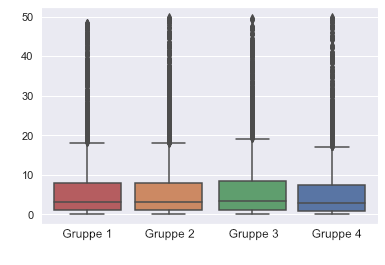
\includegraphics[width=0.8\textwidth]{contents/06_model_evaluation/res/OffRoute_Result_Overview.png}
    \caption{Anzahl der Offroutes pro Kilometer für jede Studiengruppe}
\end{figure}

\begin{table}
    \begin{center}
        \begin{tabular}{|l|c|c|}
            \hline
            \textbf{Studiengruppe}  & \textbf{Mittelwert} [N/km] & \textbf{Standardabweichung} [N/km]\\ \hline
            Gruppe 1                & 0.0753 & 0.1293 \\ \hline
            Gruppe 2                & 0.0786 & 0.1272 \\ \hline
            Gruppe 3                & 0.0803 & 0.1410 \\ \hline
            Gruppe 4                & 0.0732 &  0.1328 \\ \hline
        \end{tabular}
    \end{center}
    \caption{Übersicht der Ergebnisse der Routen-Abweichungen pro Kilometer}
    \label{tab:study_offroute_results}
\end{table}

Um zu prüfen, ob die Unterschiede der Mittelwerte signifikant sind, muss dies mittels eines statistischen Tests überprüft werden. Da es sich um ein Experiment von meheeren nicht zusammenhängenden Studiengruppen mit mehr als zwei verschiedenen Bedingungen handelt, kommen entweder ein ANOVA- oder Kruskal-Wallis-Test infrage. Für ersteren gilt, dass die Daten gleich verteilt sein müssen. Dies wurde mittels Shapiro-Wilk-Test geprüft. Da das Ergebnis für alle Test-Gruppen $ p = 0.0 < 0.05 $ ist, sind die Daten nicht normal verteilt. Folglich wird zur Signifikanzprüfung der Kruskal-Wallis-Test verwendet. Aufgrund des Ergebnisses von $ p = 0.000007 < 0.05 $, wird abgeleitet, dass ein Haupteffekt vorliegt.

Für die Prüfung zwischen welchen Studiengruppen ein signifikanter Unterschied vorliegt, wird der Dunn-Test \cite{dunn1964multiple} verwendet. (P wird mit der \glqq bonferoni\grqq{}-Methode korrigiert.)

Auch hier wird wieder von einem Signifikanzniveau $ p < 0.05 $ ausgegangen (Siehe \autoref{sec:appendix_study_results}). Folglich weichen die Nutzer der Gruppe 4 signifikant weniger von der vorgeschlagenen Route ab als die Teilnehmer aller anderen Gruppen ($ p_{11} = 0.0288 $, $ p_{12} = 0.0000 $, $ p_{13} = 0.0030 $). Weitere signifikante Unterschiede gibt es nicht.

Hypothese 2.1 trifft zwar für das Geben aller Erklärungstypen (Gruppe 4) zu, nicht aber für die Gruppen 2 und 3. Folglich wird diese abgelehnt. Hypothese 2.2 kann angenommen werden, da die Nutzer der Gruppe 4 sowohl signifikant weniger von der vorgeschlagenen Route abgewichen sind als die Nutzer der Gruppe 2 sind als auch die Nutzer der Gruppe 3.

\subsubsection{Nutzerzufriedenheit mit der aktuellen Route}

Um die Zufriedenheit der Nutzer mit der abgeschlossenen Navigation zu evaluieren, setzt NUNAV auf eine Bewertung mithilfe von 5 Sternen bei Erreichen des Zieles. Dies ist verknüpft mit der Frage \glqq Wie hat dir die Fahrt gefallen\grqq (Siehe \autoref{fig:screenshot_destination_reached}). Außerdem sind die Fahrtdauer und zurückgelegte Kilometer angegeben.

\begin{figure}[bth]
    
\includegraphics[width=0.25\linewidth]{contents/res/missing_image.pdf}
    \caption{Bildschirmfoto der Bewertungsdialogs}
    \label{fig:screenshot_destination_reached}
\end{figure}

\textbf{Hypothesen}

\begin{enumerate}
    \item[3.1] WENN Teilnehmer Erklärungen erhalten, DANN geben sie im Vergleich eine signifikant höhere Bewertung für die Navigation ab, als wenn sie keine Erklärungen erhalten.
    \item[3.2] WENN Teilnehmer nur einen der beiden vorgestellten Erklärungstypen erhalten, DANN geben sie im Vergleich eine signifikant niedrigere Bewertung für die Navigation ab, als wenn sie beide Erklärungstypen erhalten.
\end{enumerate}

\begin{figure}[bth]!
    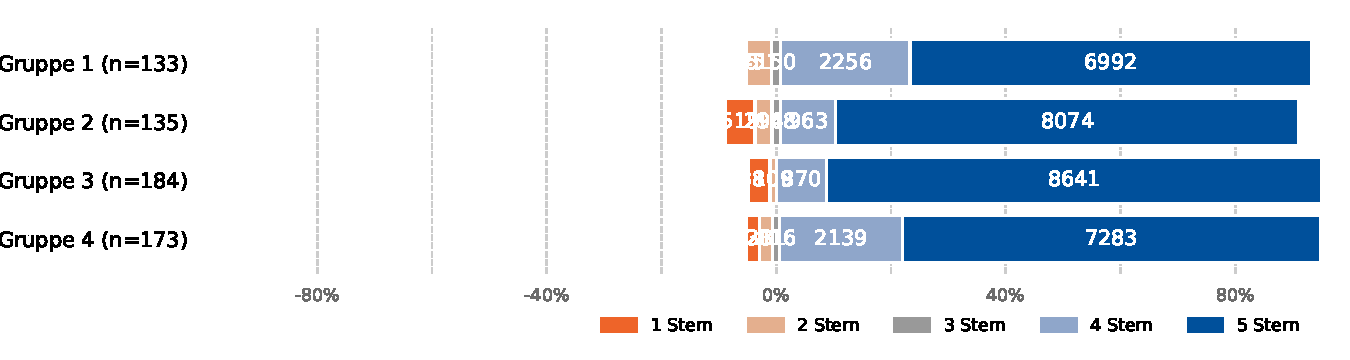
\includegraphics[width=\linewidth]{contents/06_model_evaluation/res/Rating_Result_Overview.pdf}
    \caption{Verteilung der Teilnehmer-Bewertung der Navigation für jede Studiengruppe bezogen auf die insgesamt abgegebenen Bewertungen}
    \label{fig:Rating_Result_Overview}
\end{figure}

Für die Prüfung zwischen welchen Studiengruppen ein signifikanter Unterschied vorliegt, wird wieder der Dunn-Test \cite{dunn1964multiple} verwendet, nachdem ein Kruskal-Wallis-Test einen Haupteffekt zeigt ($ p = 0.00335 $). Daraus resultiert, dass es zwischen den Gruppen 1 und 3 ($ p = 0.005723$) sowie 3 und 4 ($ p = 0.024375 $) einen signifikanten Unterschied bei der Zufriedenheit mit der aktuellen Route gibt. Mithilfe von \autoref{fig:Rating_Result_Overview} wird abgeleitet, dass es insbesondere mehr 5-Stern-Bewertungen in Gruppe 3 gegenüber den Gruppen 1 und 4 gibt. Die Anteile der ein und zwei Stern Bewertungen unterscheiden sich kaum. Folglich kann man sagen, dass die Teilnehmer signifikant zufriedener mit der Navigation waren, wenn sie Erklärungen wie in Gruppe 3 bekommen im Vergleich zu keinen Erklärungen (Gruppe 1) oder allen vorgestellten Erklärungstypen (Gruppe 4).

Da beim Geben von Erklärungen dies die Nutzerzufriedenheit nicht in jedem Fall erhöht, muss Hypothese 3.1 abgelehnt werden. Hypothese 3.2 muss ebenfalls abgelehnt werden, unter anderem da es einen gegenteiligen Effekt zwischen den Gruppen 3 und 4 gibt.

\subsubsection{Häufigkeit der Nutzung}
\label{sec:06_model_evaluation:usage_analysis}

Bei der Analyse der Nutzungshäufigkeit von NUNAV wird über den zweiwöchigen Studienzeitrum geprüft, wie viele Routen pro Nutzer und Studiengruppe in diesem Zeitraum gefahren wurden.

\textbf{Hypothesen}

\begin{enumerate}
    \item[4.1] WENN Teilnehmer Erklärungen erhalten, DANN verwenden sie NUNAV signifikant häufiger, als wenn sie keine erhalten.
    \item[4.2] WENN Teilnehmer nur einen der beiden vorgestellten Erklärungstypen erhalten, DANN nutzen sie NUNAV signifikant seltener, als wenn sie beide Erklärungstypen erhalten.
\end{enumerate}

Bei der Betrachtung der Anzahl der gefahrenen Routen werden die Daten zunächst normalisiert. Folglich sind 3 951 Nutzer im Datensatz für die Prüfung der Hypothesen verblieben.

\begin{figure}[bth]!
    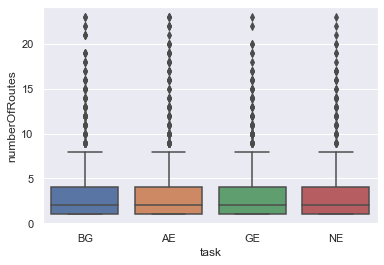
\includegraphics{contents/06_model_evaluation/res/Usage_Result_Overview.png}
    \caption{Anzahl der gefahrenen Routen für jede Studiengruppe}
\end{figure}

\begin{longtable}{|c|c|c|c|}
    \hline
    \textbf{Studiengruppe}  & \textbf{Mittelwert} [N] & \textbf{Standardabweichung} [N] \\ \hline
    Gruppe 1                & 3.2672 & 3.2958 \\ \hline
    Gruppe 2                & 3.2256 & 3.1961 \\ \hline
    Gruppe 3                & 4.6630 & 4.7043 \\ \hline
    Gruppe 4                & 4.5391 & 4.1509 \\ \hline
\caption{Übersicht der Ergebnisse der gefahrenen Routen der Nutzer}
\label{tab:study_offroute_results_2}
\end{longtable}

Zur Prüfung der Signifikanz wird wieder der Kruskal-Wallis-Test eingesetzt, da auch die Daten der Anzahl der gefahrenen Routen pro Studienteilnehmer nicht normalverteilt sind (Shapiro-Wilk: $ p = 0.0000 < 0.05 $). Mit $ p = 1.146748e-16 $ kann davon ausgegangen werden, dass ein Haupteffekt vorliegt.

Für die Prüfung zwischen welchen Studiengruppen ein signifikanter Unterschied vorliegt, wird auch hier der Dunn-Test verwendnet. Die Prüfung ergibt, dass jeweils ein signifikanter Effekt zwischen den Gruppen 3 und 4 gegenüber den Gruppen 1 und 2 vorliegt. Folglich kann abgeleitet werden, dass die Nutzer NUNAV häufiger verwenden, wenn sie die Erklärungen während der Navigation erhalten unabhängig davon, ob diese kombiniert mit den Erklärungen vor der Navigation erfolgen.

Die Hypothesen 4.1 und 4.2 müssen abgelehnt werden, da weder alle Erklärungstypen zu einer signifikant häufigeren Nutzung von NUNAV führen, noch das Geben von beiden vorgestellten Typen von Erklärungen zu einer erhöhten Nutzung pro Studienteilnehmer führt im Vergleich zur Präsentation von nur einem der integrierten Erklärungstypen.

\chapter{Diskussion}

Ziel der vorliegenden Arbeit war die Entwicklung eines Modells bzw. Richtlinien zur Unterstützung bei der Gestaltung von Erklärungen. Innerhalb dieser Arbeit ist ein Leitfaden entstanden, welcher die geforderte Unterstützung liefern soll. In diesem Kapitel wird die Anwendbarkeit des Leitfadens in der Wirtschaft analysiert. Darüber hinaus wird die Allgemeingültigkeit des enthaltenen Modells und des Katalogs der Zusammenhänge diskutiert, sowie die Limitierungen der Evaluation der Erklärungen aufgezeigt. Außerdem werden die Herausforderungen dieser Arbeit vorgestellt.

\section{Interpretation der Ergebnisse}

\subsection*{Beantwortung der Forschungsfragen}

Mit einem Modell für die Aspekte von Erklärungen, den Zusammenhängen und Einflüssen auf ausgewählte externe Qualitätsaspekte sowie Heuristiken zur Gestaltung von Erklärungen ist zusammenfassend ein Leitfaden zur Unterstützung von Erklärunge

\subsection*{Bewertung des Leitfadens für die Integration von Erklärungen}

Anhand der Rückfragen zum Leitfaden für die Integration von Erklärungen konnte abgeleitet werden, dass dieser zum Zeitpunkt des Workshops nur wenige offensichtliche Unverständlichkeiten aufwies. Lediglich die verschiedenen Inhaltstypen von Erklärungen haben nicht alle Teilnehmer des Workshops direkt verstanden. Die Typen waren zu dem Zeitpunkt noch als Fragewörter voneinander abgegrenzt, was für das finale Modell in der Folge geändert wurde (siehe \autoref{fig:model_overview_complete}).

Diese können folglich ohne ernste Bedenken über die Studie hinaus in \textit{NUNAV Navigation} integriert bleiben.

Der Leitfaden an sich enthält keine Einführung in Erklärbarkeit, diese wurde aber im Rahmen einer Präsentation als Einführung des Workshops gegeben. Dabei ist aufgefallen, dass eine wichtige Verständnisfrage für die Teilnehmer war, wo die genaue Abgrenzung zwischen Erklärbarkeit und gutem User-Interface-Design ist. Für die Anwendung des Leitfadens wird dieses Wissen über Erklärbarkeit vorausgesetzt. Folglich hat in diesem Fall eine Einführung in das Thema Erklärbarkeit sehr geholfen.

Außerdem ist als Beobachter aufgefallen, dass insbesondere die verschiedenen Möglichkeiten, Erklärungen zu gestalten aus dem Leitfaden die Diskussion über Umsetzungsideen angeregt haben. Da eines der Ergebnisse war, dass die Evaluation vor allem durch Verhaltensmetriken erfolgen sollte, konnten viele der im Leitfaden vorgestellten qualitativen Metriken nicht zum Einsatz kommen.

es konnten nicht für jeden Nutzer alle Fragen beantwortet werden. Lösung -> Support Desk innerhalb der App.

\section{Limitierungen des Leitfadens für Erklärungen}

Der in dieser Arbeit entwickelte Leitfaden für die Integration von Erklärungen in Softwaresysteme fasst bereits gezeigte Ergebnisse zusammen und strukturiert diese. Folglich sind in dem entstandenen Modell für Erklärungen, dem Katalog über die Einflüsse von Erklärungen auf bestimmte Qualitätsaspekte und den daraus abgeleiteten Design Heuristiken keine neuen Ergebnisse entstanden, sondern nur bestehende Resultate in einen Zusammenhang gestellt worden. 
Der Leitfaden erhebt allerdings keinen Anspruch auf Vollständigkeit. Vor allem für spezifische Kontexte bieten bereits entwickelte Modelle einen tieferen Einblick \cite{nunes_systematic_2017, sokol_explainability_2020}.

Eine weitere Limitierung, die bei der Entwicklung des Leitfadens auf Basis einer Literaturrecherche gemacht werden muss, ist, dass diese nur von einer Person durchgeführt und daher nicht überprüft wurde. Daher können Aspekte übersehen oder fehlerhaft eingeordnet worden sein. Dies unterscheidet die im Rahmen dieser Arbeit durchgeführte Literaturrecherche vor allem von bereits durchgeführten systematischen Literaturrecherchen zum Thema \textit{Explainability} \cite[vgl.][]{nunes_systematic_2017,chazette_knowledge_nodate}.

In dieser Arbeit wurde versucht, den Leitfaden ganzheitlich als Methode in der Wirtschaft anzuwenden. Dabei hat sich herausgestellt, dass nicht alle Teile des Leitfadens für jedes Team einsetzbar sind. Beispielsweise wurden die Ziele zur Integration von Erklärungen von Graphmasters sehr allgemein gehalten, da eine Konkretisierung der Ziele zum Beispiel mittels Qualitätsmodellen \cite{schneider2012abenteuer} in den Prozessen des Unternehmens nicht vorgesehen ist. Um allerdings den Katalog der Zusammenhänge des Leitfadens anzuwenden wurden die Anforderungen im Rahmen dieser Arbeit trotz dessen konkretisiert und mit Graphmasters abgesprochen. Auch kommen nicht immer alle Evaluationsmöglichkeiten des Modells für einen Kontext infrage, da es äußere Beschränkungen gibt (siehe \autoref{sec:02_evaluation_explanations}).

Als Einschränkung für die Allgemeingültigkeit des Leitfadens muss auch erwähnt werden, dass der Einsatz mit dieser Arbeit nur in einem agil arbeitenden Unternehmen im \textit{Context} von mobilen Anwendungen untersucht wurde. Die Ergebnisse, in welchen Bereichen Teile des Leitfadens sinnvoll eingesetzt werden können, sind folglich nicht verallgemeinerbar.

Eine weitere Einschränkung bei der Verallgemeinerung des Leitfadens ist, dass keine direkte Evaluation des Leitfadens erfolgt ist. Diese ist nur indirekt durch die Anwendung des Leitfadens geschehen. Es können folglich Verständnisprobleme oder Herausforderungen bei der Nutzung in verschiedenen Prozessen bei der Entwicklung von Erklärungen auftreten.

Für die Verallgemeinerbarkeit des Leitfadens spricht, dass bei der Anwendung des Leitfadens mehrere Ergebnisse und Empfehlungen aus vorangegangenen Arbeiten reproduziert werden konnten. Beispielsweise konnte die Notwendigkeit von qualitativer und quantitativer Evaluation gezeigt werden, um interpretierbare Ergebnisse zu erlangen \cite{sokol_explainability_2020}. Auch konnte gezeigt werden, dass die Performanz der \textit{End User} durch Erklärungen erhöht und gleichzeitig die \textit{Satisfaction} sinken kann \cite{koo_understanding_2016}. 

Final bieten die Ergebnisse einen allgemeinen Überblick für die Integration von Erklärungen in erklärbare Systeme. Somit ist es für Anwender des Leitfadens möglich, anhand von Einschränkungen des eigenen \textit{Contexts} und äußeren Bedingungen die Teile des Leitfadens zu wählen, die ihnen bei der Integration von Erklärungen helfen können. Der Leitfaden bietet folglich eine gewisse Flexibilität.

\newpage



\section{Herausforderungen}

Im Folgenden werden die Herausforderungen vorgestellt, die während der Forschung für diese Arbeit entstanden sind.

Eine der Hauptaufgaben dieser Arbeit ist das Zusammentragen der bestehenden Ergebnisse zur neuen NFR \textit{Explainability} gewesen. Vor allem durch die sehr subjektiven und in verschiedenen Kontexten sehr unterschiedliche Wahrnehmung von Erklärungen war die Vereinheitlichung der Ergebnisse nicht trivial. Da vergangene Forschung vor allem einzelne Aspekte von Erklärungen ohne ein einheitliches Evaluationsschema analysiert hat, war auch die Aufstellung der Zusammenhänge zwischen den einzelnen Aspekten des in der vorliegenden Arbeit vorgestellten Leitfadens eine Herausforderung. Hier konnten vorwiegend existierende Modelle wie von \citeauthor{nunes_systematic_2017} für Erklärungen für Empfehlungssysteme und die Definition für Erklärbarkeit von \citeauthor{chazette_knowledge_nodate} eine Orientierung geben \cite{nunes_systematic_2017, chazette_knowledge_nodate}. Aufgrund der Diversität von \textit{Explainability} sind auch weniger allgemeine Resultate im Rahmen dieser Arbeit entstanden als zu Beginn der Literaturrecherche erwartet. Daher bietet der Leitfaden vordergründig einen Überblick über verschiedene Aspekte von Erklärungen sowie der Zusammenhänge.

Neben den Herausforderungen bei der Entwicklung des Leitfadens sind während dem Technologietransfer in die Praxis weitere Hürden zu überwinden gewesen. Der Leitfaden ist mit Zielen konzipiert, welche für die Anwendung in Qualitätsmodellen zur Ableitung von Anforderungen dienen. Die agile Arbeitsweise von \textit{Graphmasters} ist allerdings nicht für eine konkrete Anforderungserhebung ausgelegt. Daher war diese Methode unbekannt. Folglich bedurfte die Festlegung der konkreten und überprüfbaren in Absprache mit \textit{Graphmasters} einem besonderen Augenmerk. Insbesondere das Festlegen von Sollwerten für die entwickelten Metriken konnte nicht erfolgen. Hier wurde der Unterschied zwischen in der Wissenschaft entwickelten Modellen und Verwendung in der Wirtschaft deutlich gezeigt. Trotz dessen hatte der entwickelte Leitfaden eine unterstützende Wirkung für die Aktivitäten der Integration von Erklärungen (Anforderungserhebung, Umsetzung, Evaluation). Auch konnten statistisch überprüfbare Qualitätsanforderungen formuliert werden (siehe \autoref{sec:explanation_requirements}). Für eine erneute Verwendung des Leitfadens bei \textit{Graphmasters} muss allerdings eine bessere Integration in den agilen Prozess von \textit{Graphmasters} erfolgen.

\chapter{Fazit und Ausblick}

\section{Fazit}

Ziel dieser Arbeit war es, ein Modell zur Unterstützung des Designs von Erklärungen in erklärbaren Systemen zu konzipieren und im Anschluss zu evaluieren. Als Ergebnis dieser Arbeit ist unter anderem einen ein Modell zur Unterstützung der Integration von Erklärungen entstanden, welches in einen Leitfaden integriert ist. Der Leitfaden enthält darüber hinaus einen Katalog über bestehende und verallgemeinerbare Zusammenhänge zwischen den äußeren Abhängigkeiten für Erklärungen, den Eigenschaften und Einflüssen auf die Softwarequalität. Abschließend werden im Leitfaden außerdem einige wichtige Heuristiken für das Design von Erklärungen zusammengefasst. Dieser ist im Rahmen einer Literaturrecherche entstanden, welche die bestehenden Ergebnisse für das Design von Erklärungen in erklärbaren Systemen analysiert hat. Der im Leitfaden für die Integration von Erklärungen enthaltene Modell beinhaltet dabei die folgenden Teile:

\paragraph{RQ1} Unter \textit{External Dependencies} sind alle Rahmenbedingungen zusammengefasst, die einen direkten Einfluss auf die Anforderungen an Erklärungen aufweisen. Als relevante Aspekte sind verschiedene Ausprägungen des \textit{Contexts} von erklärbaren Systemen, sowie \textit{Objectives} auf verschiedenen Abstraktionsebenen für die Integration von Erklärungen in dem Modell enthalten. Somit unterstützt dieser Modellteil die Anforderungserhebung für Erklärungen.

\paragraph{RQ2} 

\smallskip

\noindent\fbox{
    \parbox{0.964\textwidth}{
        \smallskip
        \textbf{RQ1} Welche Rahmenbedingungen haben einen Einfluss auf die Anforderungen für Erklärungen?
        \smallskip
    }
}

\smallskip

\noindent\fbox{
    \parbox{0.964\textwidth}{
        \smallskip
        \textbf{RQ2} Welche Eigenschaften von Erklärungen haben einen Einfluss auf die externe Qualität eines erklärbaren Systems?
        \smallskip
    }
}

\smallskip

Der in diesem Abschnitt vorgestellte Teil des Modells für Erklärungen (\textit{Characteristics}) beinhaltet die Antwort auf die zweite Forschungsfrage. Dabei sind explizit die Eigenschaften \textit{Demand}, \textit{Content} und \textit{Presentation} mit einem Einfluss auf die externe Qualität von Erklärungen zu benennen. Die genauen Ausprägungen dieser Eigenschaften werden als Unterpunkte der jeweiligen Aspekte im Modell enthalten. Die Ergebnisse, die in dem Modell zusammengefasst sind, entspringen dabei der Evaluation von Erklärungen mit verschiedenen Eigenschaften in der Literatur.

\smallskip

\noindent\fbox{
    \parbox{0.964\textwidth}{
        \smallskip
        \textbf{RQ3} Auf welche Art und Weise kann evaluiert werden, ob die in ein erklärbares System integrierten Erklärungen das Ziel der Integration bezogen auf externe Qualitätsaspekte erfüllt haben?
        \smallskip
    }
}

\smallskip

Der Abschnitt \textit{Evaluation} des Modells für Erklärungen ist die Antwort auf die dritte Forschungsfrage. Dies erfolgt in drei Teilen. Zunächst enthält das Modell einen kurzen Überblick über das Studiendesign für verschiedene Anwendungsfälle. Außerdem sind Teil der Antwort die zwei verschiedene Evaluationsmöglichkeiten: direkte Erklärungsevaluation und Evaluation der Auswirkungen auf das System im Allgemeinen. Für beide Varianten werden in dem Modell Beispiele für qualitative und quantitative Betrachtungen genannt. Dies erfüllt auch die Anforderung an den Leitfaden ([GR3])

Zusammenfassend kann gesagt werden, dass für ein ganzheitliches Bild über die Qualität von Erklärungen sowohl qualitativ als auch quantitativ die Erklärungen an sich sowie dessen Auswirkung auf weitere externe Qualitätsaspekte betrachtet werden müssen \cite{balog_measuring_2020}. Wichtig ist dabei auch die Betrachtung von Aspekten zur Kontrolle, auf die ggf. negative Effekte durch Erklärungen möglich sind.

\smallskip

\noindent\fbox{
    \parbox{0.964\textwidth}{
        \smallskip 
        \textbf{RQ4.2} Welchen Einfluss hat die Granularität von Erklärungen auf die externe Qualität eines erklärbaren Systems unter bestimmten Rahmenbedingungen?
        \smallskip
    }
}

\smallskip

Die Einflüsse, die Eigenschaften der Granularität von Erklärungen auf einige externe Qualitätsaspekte haben, werden im zweiten Teil des Katalogs der Zusammenhänge der Aspekte von Erklärungen, zusammengestellt. Ebenfalls wird somit eine Antwort auf die letzte Forschungsfrage gegeben und erfüllt die Anforderung GR4, welche fordert, dass der Leitfaden eine Unterstützung bei der Auswahl von Eigenschaften bei der Umsetzung von Erklärungen geben soll.

% RQ 1 - 4 durchgehen und die ERgebnisse noch mal kürzer und knackiger zusamenfassen

% \section{Einordnung der Ergebnisse}

% \subsection{Beantwortung der Forschungsfragen}

% In dieser Arbeit 

% Mit einem Modell für die Aspekte von Erklärungen, den Zusammenhängen und Einflüssen auf ausgewählte externe Qualitätsaspekte sowie Heuristiken zur Gestaltung von Erklärungen ist zusammenfassend ein Leitfaden zur Unterstützung von Erklärungen

% Aus Studie nochmals klar geworden, dass nur mit Verhaltensmetriken, sobald diese nicht eindeutig sind, und direkt die \glqq richtige\grqq{} Erklörung getroffen wurde, die Erklärungen nicht analysiert werden können.

Final hat der Leitfaden bei allen wichtige Schritten der Integration von Erklärungen (Anforderungserhebung, Umsetzung und Evaluation) geholfen. Darüber hinaus wurden unter Anwendung des Leitfadens positive Einflüsse auf die zuvor gesetzten Ziele erzielt worden. 

\section{Ausblick}

% Our long-term vision is to establish a standardized certification process in tandem with appropriate development techniques to achieve explainability by design. This paper is a starting point towards an overarching and systematic approach to explainability requirements. Unknown source


Es fehlt: A framework for integrating explanatory capabilities in the whole software development life-cycle, from requirements elicitation over design and implementation through to its use \cite{cassens_ambient_2019}

need studys for obtrusiveness \cite{lim_2009_assessing}

Conclusion: Es fehlen noch Artefakte für... z.B. aus den im Modell gesammelten Möglichkeiten der Evaluation muss noch ein konkretes Framework gebaut werden, wie es von \citeauthor{sokol_explainability_2020} gefordert wird.

Es fehlt ein klarer Explainability SIG wie auch für Transparency \cite{do2010software} und Invisibility \cite{carvalho2020developers}. m Entwickler einfacher supporten zu können, sollte also vor allem für die Objectives eine bessere Übersicht geschaffen werden.
Außerdem muss mehr evaluiert werden und die Vollständigkeit des Modells sollte durch mindestens eine weitere unabhngige Arbeit bestätigt werden.

Die gefahren für Usability etc. sollten besser herausgearbeitet werden -> Es wurden vor allem positiv Ergebnisse betrachtet, da in der Literatur, höufig nur die Gefahre diskutiert werden, allerdings nicht behandelt werden.

Technologietransfer, wie bei Gorschek et al.

% Es fehlt ein ausgereifter Katalog, für Zusammenhänge bei Erklärungen


\appendix

\appendix

\chapter{Anhang I}

\section{Literaturrecherche}
\label{sec:appendix_search_filter}

\begin{table}
    \centering
    \begin{tabular}{l}
        \hline
        test \\
        \toprule
        test 2 \\
        \toprule
    \end{tabular}
    \caption{Filter}
\end{table}

\begin{figure}[htb]
    \centering
    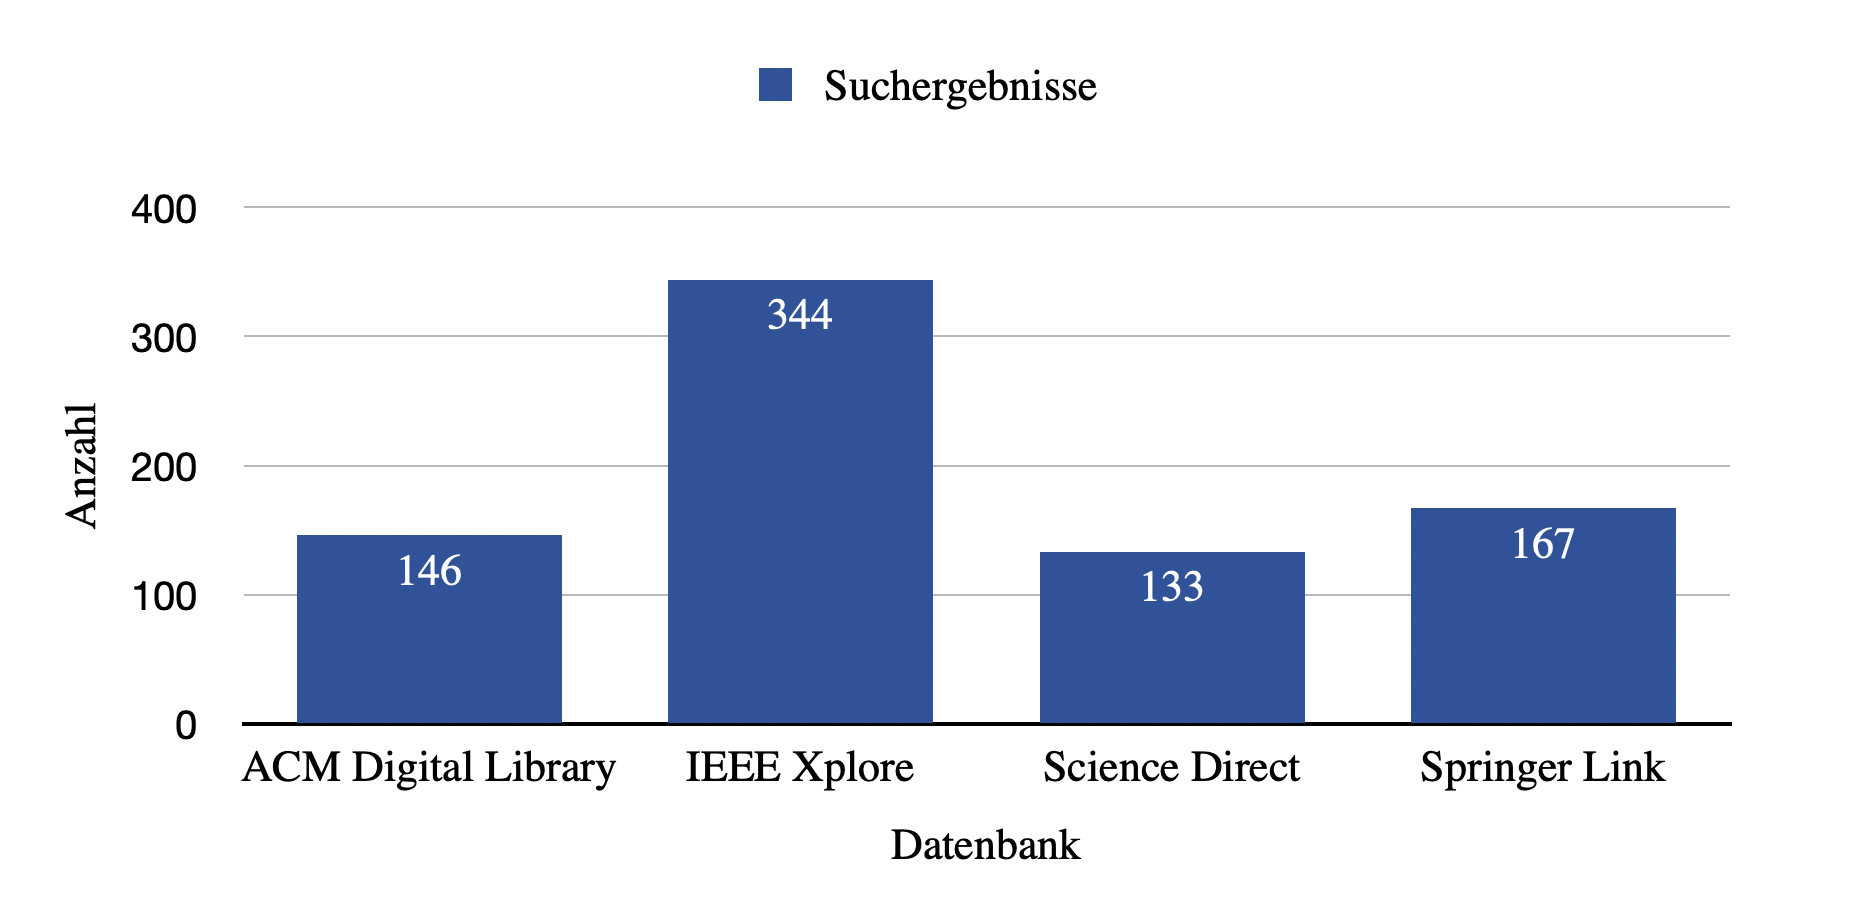
\includegraphics[width=0.75\linewidth]{contents/04_literature_review/res/database_results.png}
    \caption{Anzahl der Suchergebnisse pro Datenbank}
    \label{fig:04_literature_review_screening_process}
\end{figure}

\begin{table}
    \begin{center}
        \begin{tabular}{p{.3\textwidth}p{.64\textwidth}}
            \hline
            Kontext                   & Quellen \\
            \toprule
            Allgemein                           &
                \cite{chazette_end-users_nodate} \cite{chazette2020explainability} \cite{chazette_knowledge_nodate} \cite{eiband_impact_2019} \cite{kohl_explainability_2019} \cite{ribera2019can} \cite{lim_2009_assessing} \\
            \tablerowspacing
            Intelligente Systeme (z.B. XAI)      & 
                \cite{waa_evaluating_2021} \cite{mucha_interfaces_2021} \cite{sokol_explainability_2020}  \cite{abdulrahman_belief-based_2019} \cite{brennen_what_2020} \cite{schaffer_i_2019} \cite{weitz_you_2019} \cite{riveiro_thats_2021} \cite{martin_developing_2019} \cite{martin_evaluating_2021} \cite{rosenfeld_explainability_2019} \cite{cassens_ambient_2019} \cite{cirqueira_scenario-based_2020}  \cite{ehsan_human-centered_2020} \cite{rjoob_towards_2021} \cite{thomson_knowledge--information_2020} \cite{chari_explanation_2020} \cite{sokol_one_2020}  \cite{neerincx_using_2018} \cite{schrills_color_2020} \cite{sovrano_modelling_2020} \cite{gunning2019darpa} \cite{doshi2017towards} \cite{cheng2019explaining}\\
            \tablerowspacing
            Empfehlungssysteme                  & 
                \cite{tintarev_designing_nodate} \cite{sato_context_nodate} \cite{balog_measuring_2020}  \cite{kouki_user_2017} \cite{tsai_evaluating_2019} \cite{hernandez-bocanegra_effects_2020} \cite{kunkel_let_2019} \cite{tintarev2015explaining} \cite{sato_action-triggering_2019} \cite{tsai_effects_2020} \cite{nunes_systematic_2017} \cite{tintarev2007survey}
            \\
            \tablerowspacing
            Autonomes Fahren                    &
                \cite{wiegand_id_2020} \cite{haspiel_explanations_2018} \cite{koo_understanding_2016} \cite{koo_why_2015} \cite{wiegand2019drive} \cite{du2019look}
            \\
            \tablerowspacing
            Mensch-Roboter-Interaktion          &
                \cite{stange_effects_2021} \cite{kaptein_personalised_2017} \cite{zolotas_towards_2019} \cite{wang_is_2018} \cite{zhu_effects_2020}
            \\
            \tablerowspacing
            Spezifische Domänen                 &
                \cite{yamada_evaluating_2016} \cite{zahedi_towards_2019}
            \\
            \toprule
        \end{tabular}
    \end{center}
    \caption{Kontext innerhalb von Erklärbaren Systemen, der von den Arbeiten untersucht wurde}
    \label{tab:paer_explanation_contexts}
\end{table}


\section{Workshop}

\section{Workshop-Protokoll: Integration von Erklärungen in NUNAV}
\label{sec:appendix_workshop_protocol}

\section{Studienergebnisse}
\label{sec:appendix_study_results}

\begin{table}
    \begin{center}
        \begin{tabular}{|c|c|c|c|c|}
            \hline
            & \textbf{Gruppe 1} & \textbf{Gruppe 2} & \textbf{Gruppe 3} & \textbf{Gruppe 4} \\ \hline
            \textbf{Gruppe 1}   & 1.000000 & 1.000000 & 0.219884 & 0.008222 \\ \hline
            \textbf{Gruppe 2}   & 1.000000 & 1.000000 & 0.860586 & 0.000912 \\ \hline
            \textbf{Gruppe 3}   & 0.219884 & 0.860586 & 1.000000 & 0.000005 \\ \hline
            \textbf{Gruppe 4}   & 0.008222 & 0.000912 & 0.000005 & 1.000000 \\ \hline
        \end{tabular}
    \end{center}
    
    \caption{Signifikanzniveau $ p $ im paarweisen Vergleich der Anzahl der Routenabweichungen pro Kilometer zwischen den Studiengruppen }
    \label{tab:study_offroute_significance_results}
\end{table}

\section{Helcenter Collaborative Routing}
\label{sec:help_center_collaboratrive_routing}


\section{Helcenter Routeneinflüsse}
\label{sec:help_center_routing_data}


\section{vollständige Screenshots zum Verkehrsaufkommen}
\label{sec:appendix_traffic_volume}

\begin{figure}[htb!]
    \centering
    \subfloat[1. Prototyp zur Positionierung der \textit{Affordance}]
    {
        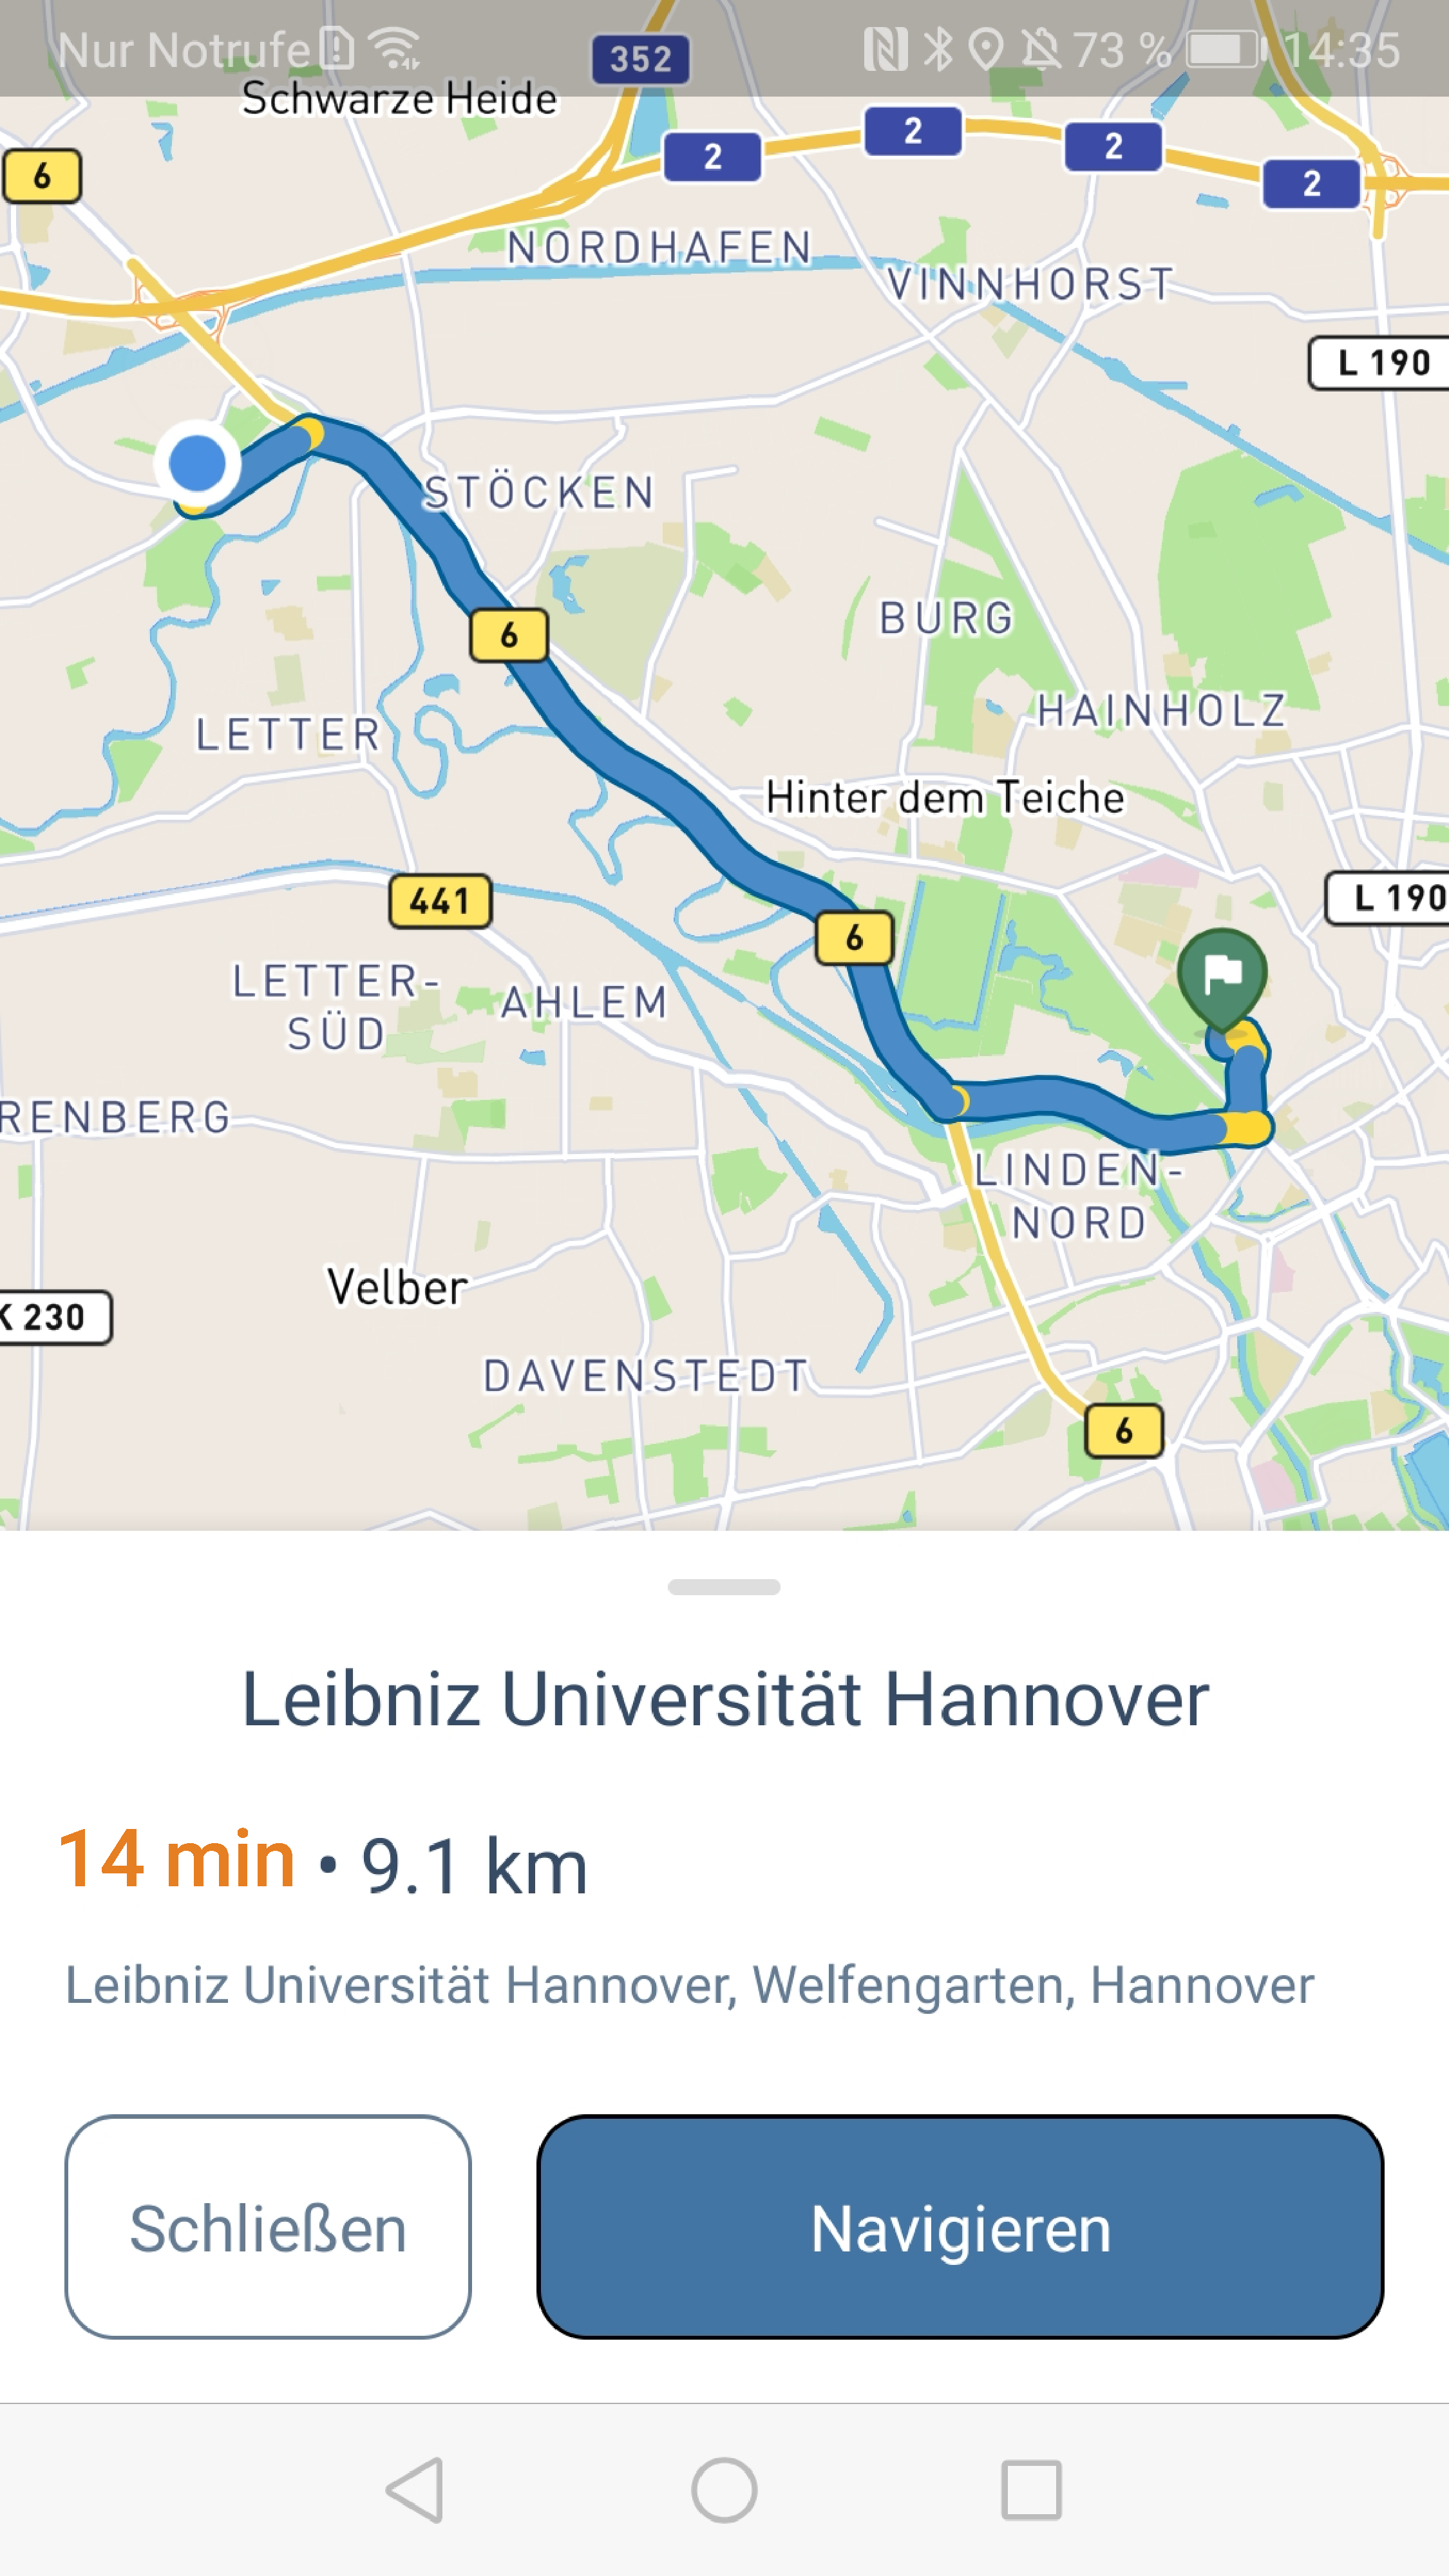
\includegraphics[width=.27\linewidth]{contents/06_model_evaluation/01_integration/res/03_traffic_volume/prototype_11.pdf}
    }
    \hspace{.055\linewidth}
    \subfloat[Alternativer Prototyp zur Positionierung der \textit{Affordance}]
    {
        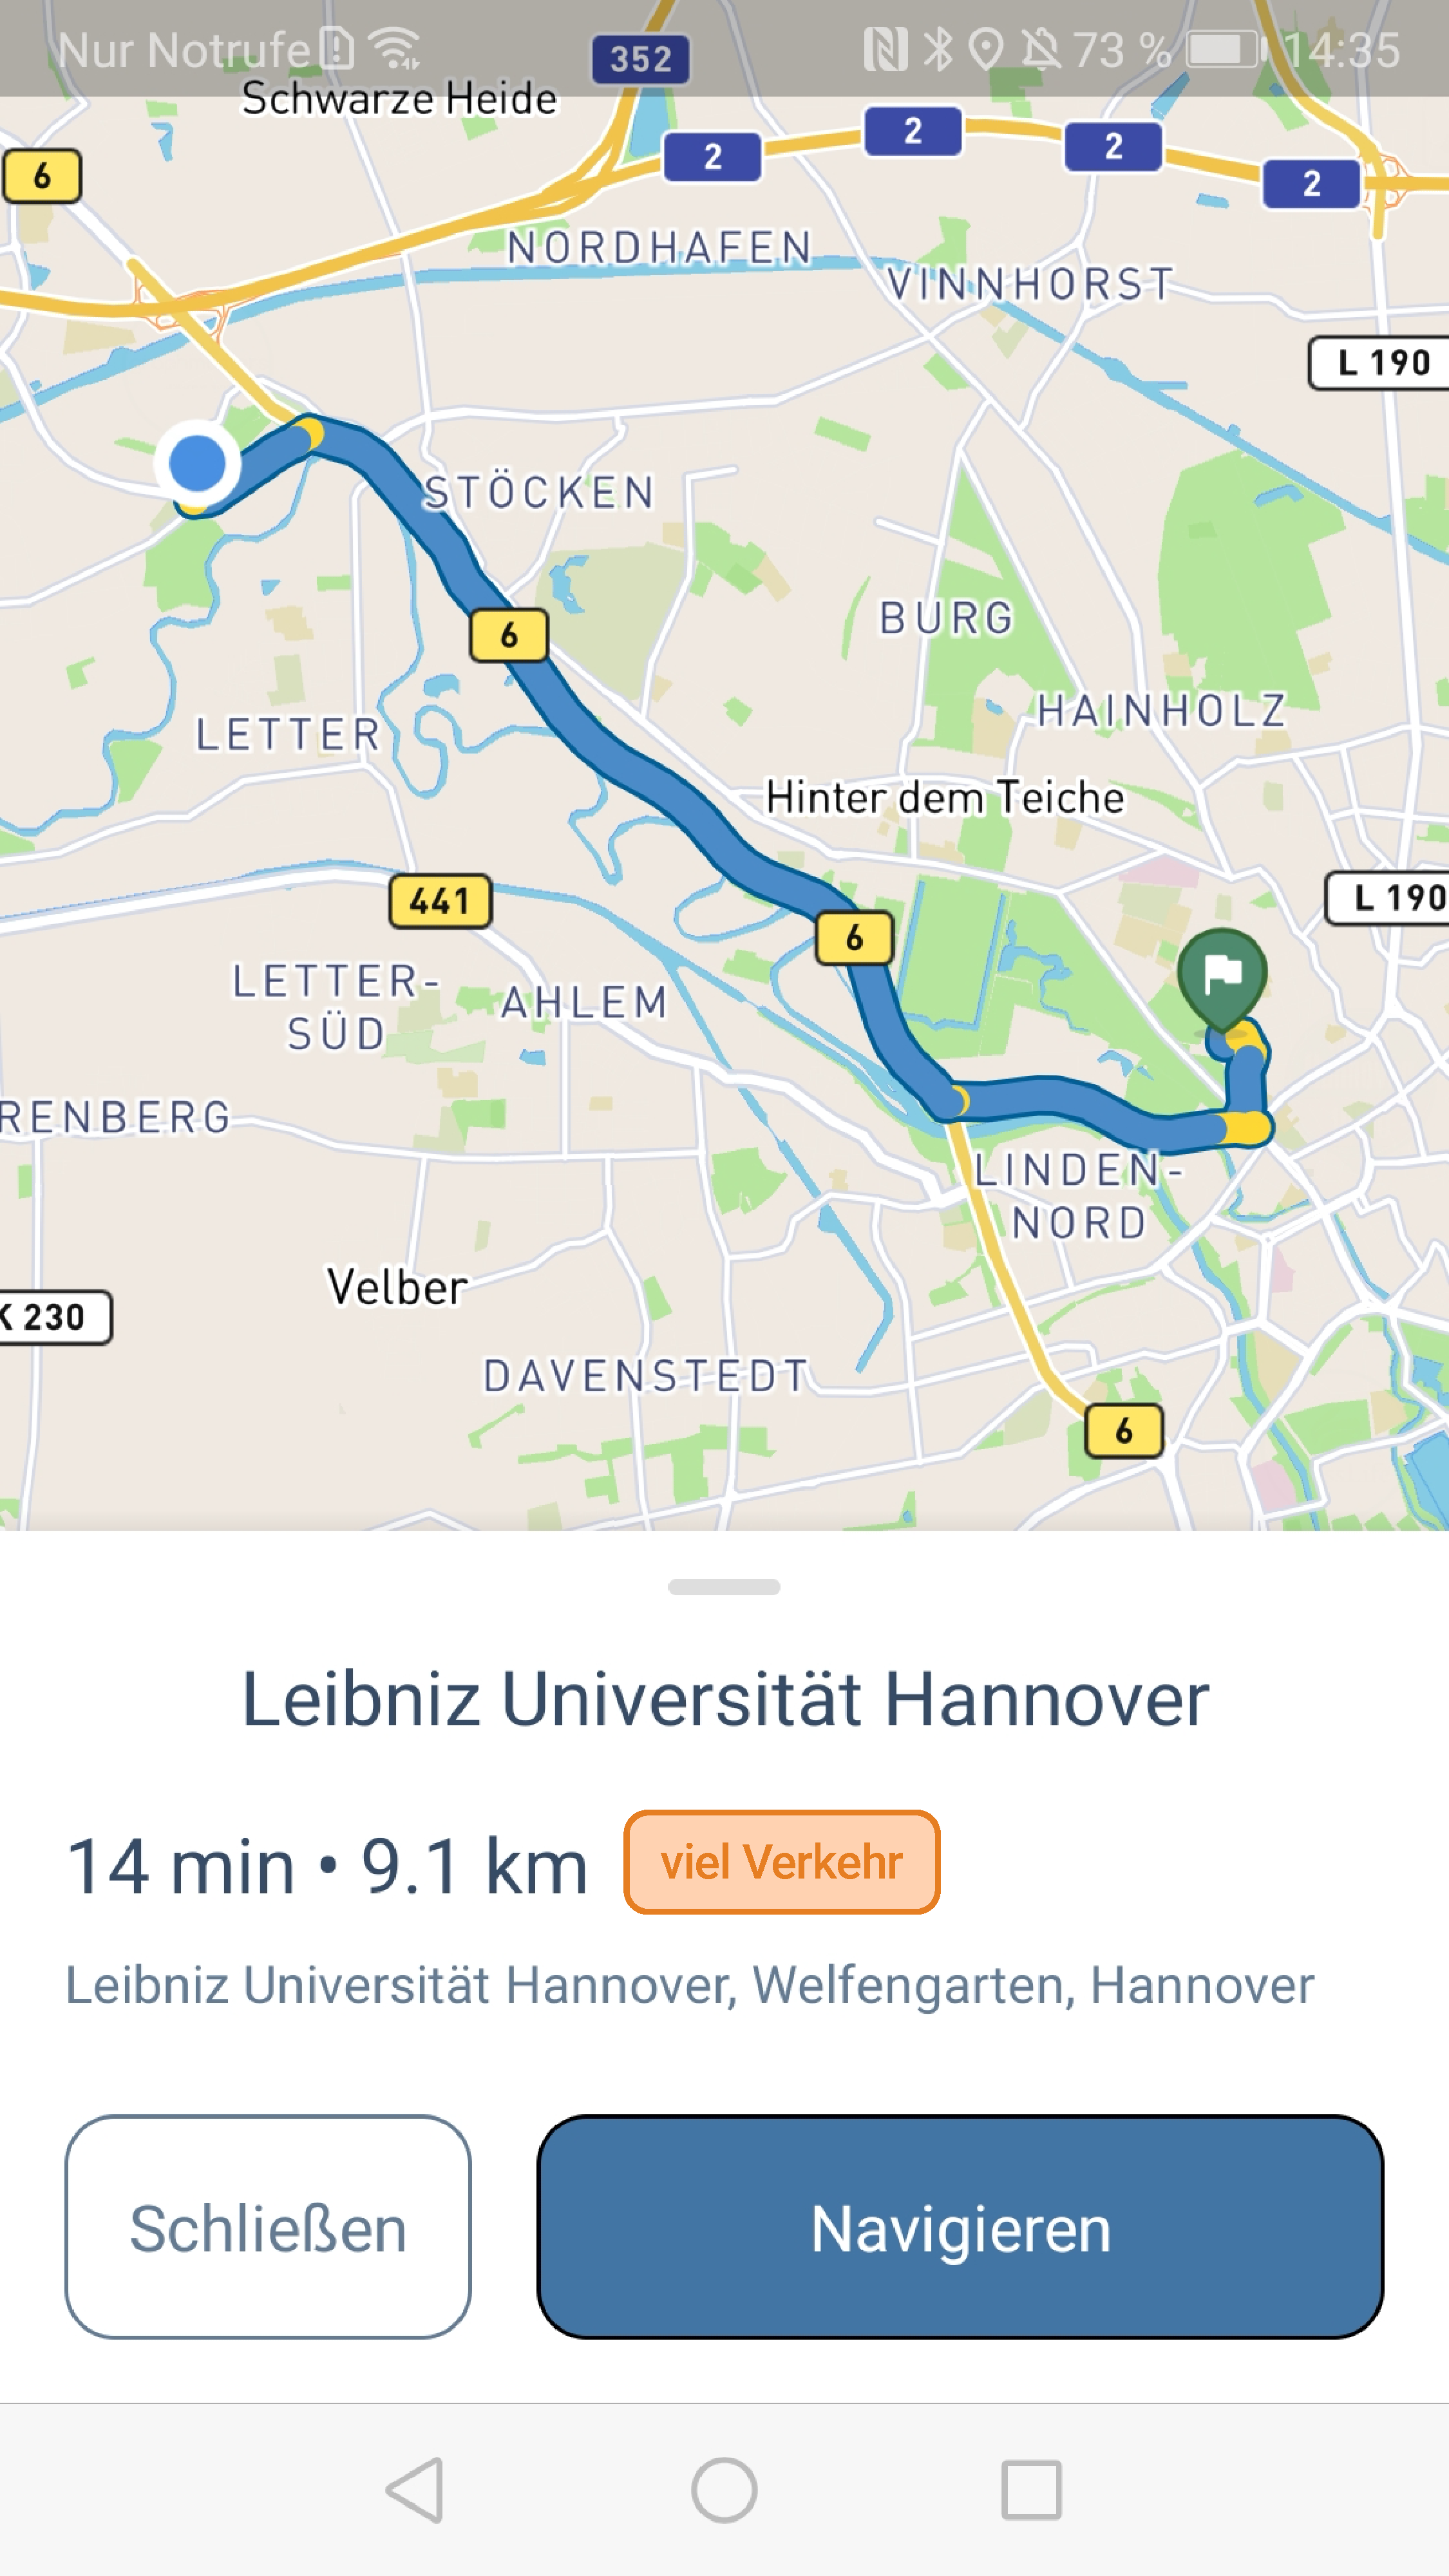
\includegraphics[width=.27\linewidth]{contents/06_model_evaluation/01_integration/res/03_traffic_volume/prototype_12.pdf}
    }
    \hspace{.055\linewidth}
    \subfloat[Finales Design der kurzen Erklärung]
    {
        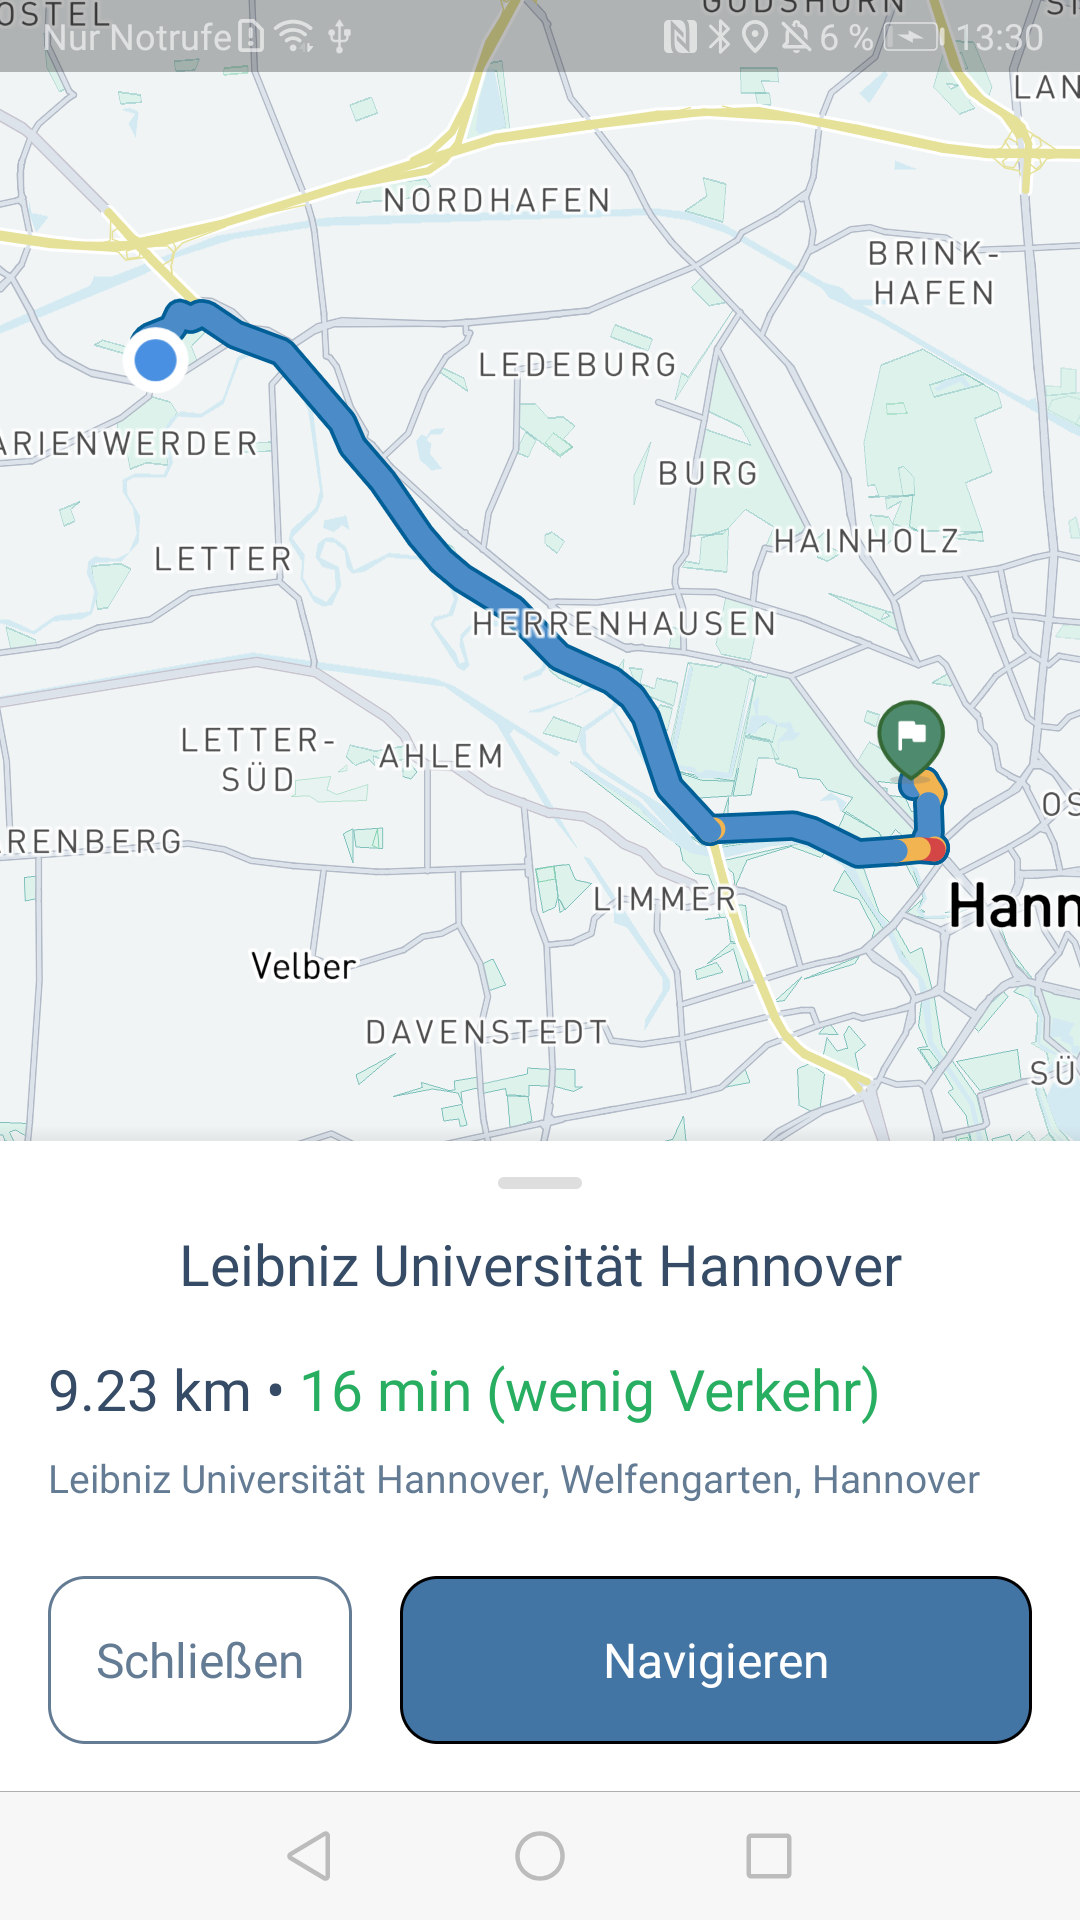
\includegraphics[width=.27\linewidth]{contents/06_model_evaluation/01_integration/res/03_traffic_volume/final_10.png}
    }
    \caption{Prototyp und finale Designs für die Erklärung zum kollaborativem Routing}
    \label{fig:prototype_traffic_volume_route_overview}
\end{figure}

\begin{figure}[htb!]
    \centering
    \subfloat[1. Prototyp zur Positionierung der \textit{Affordance}]
    {
        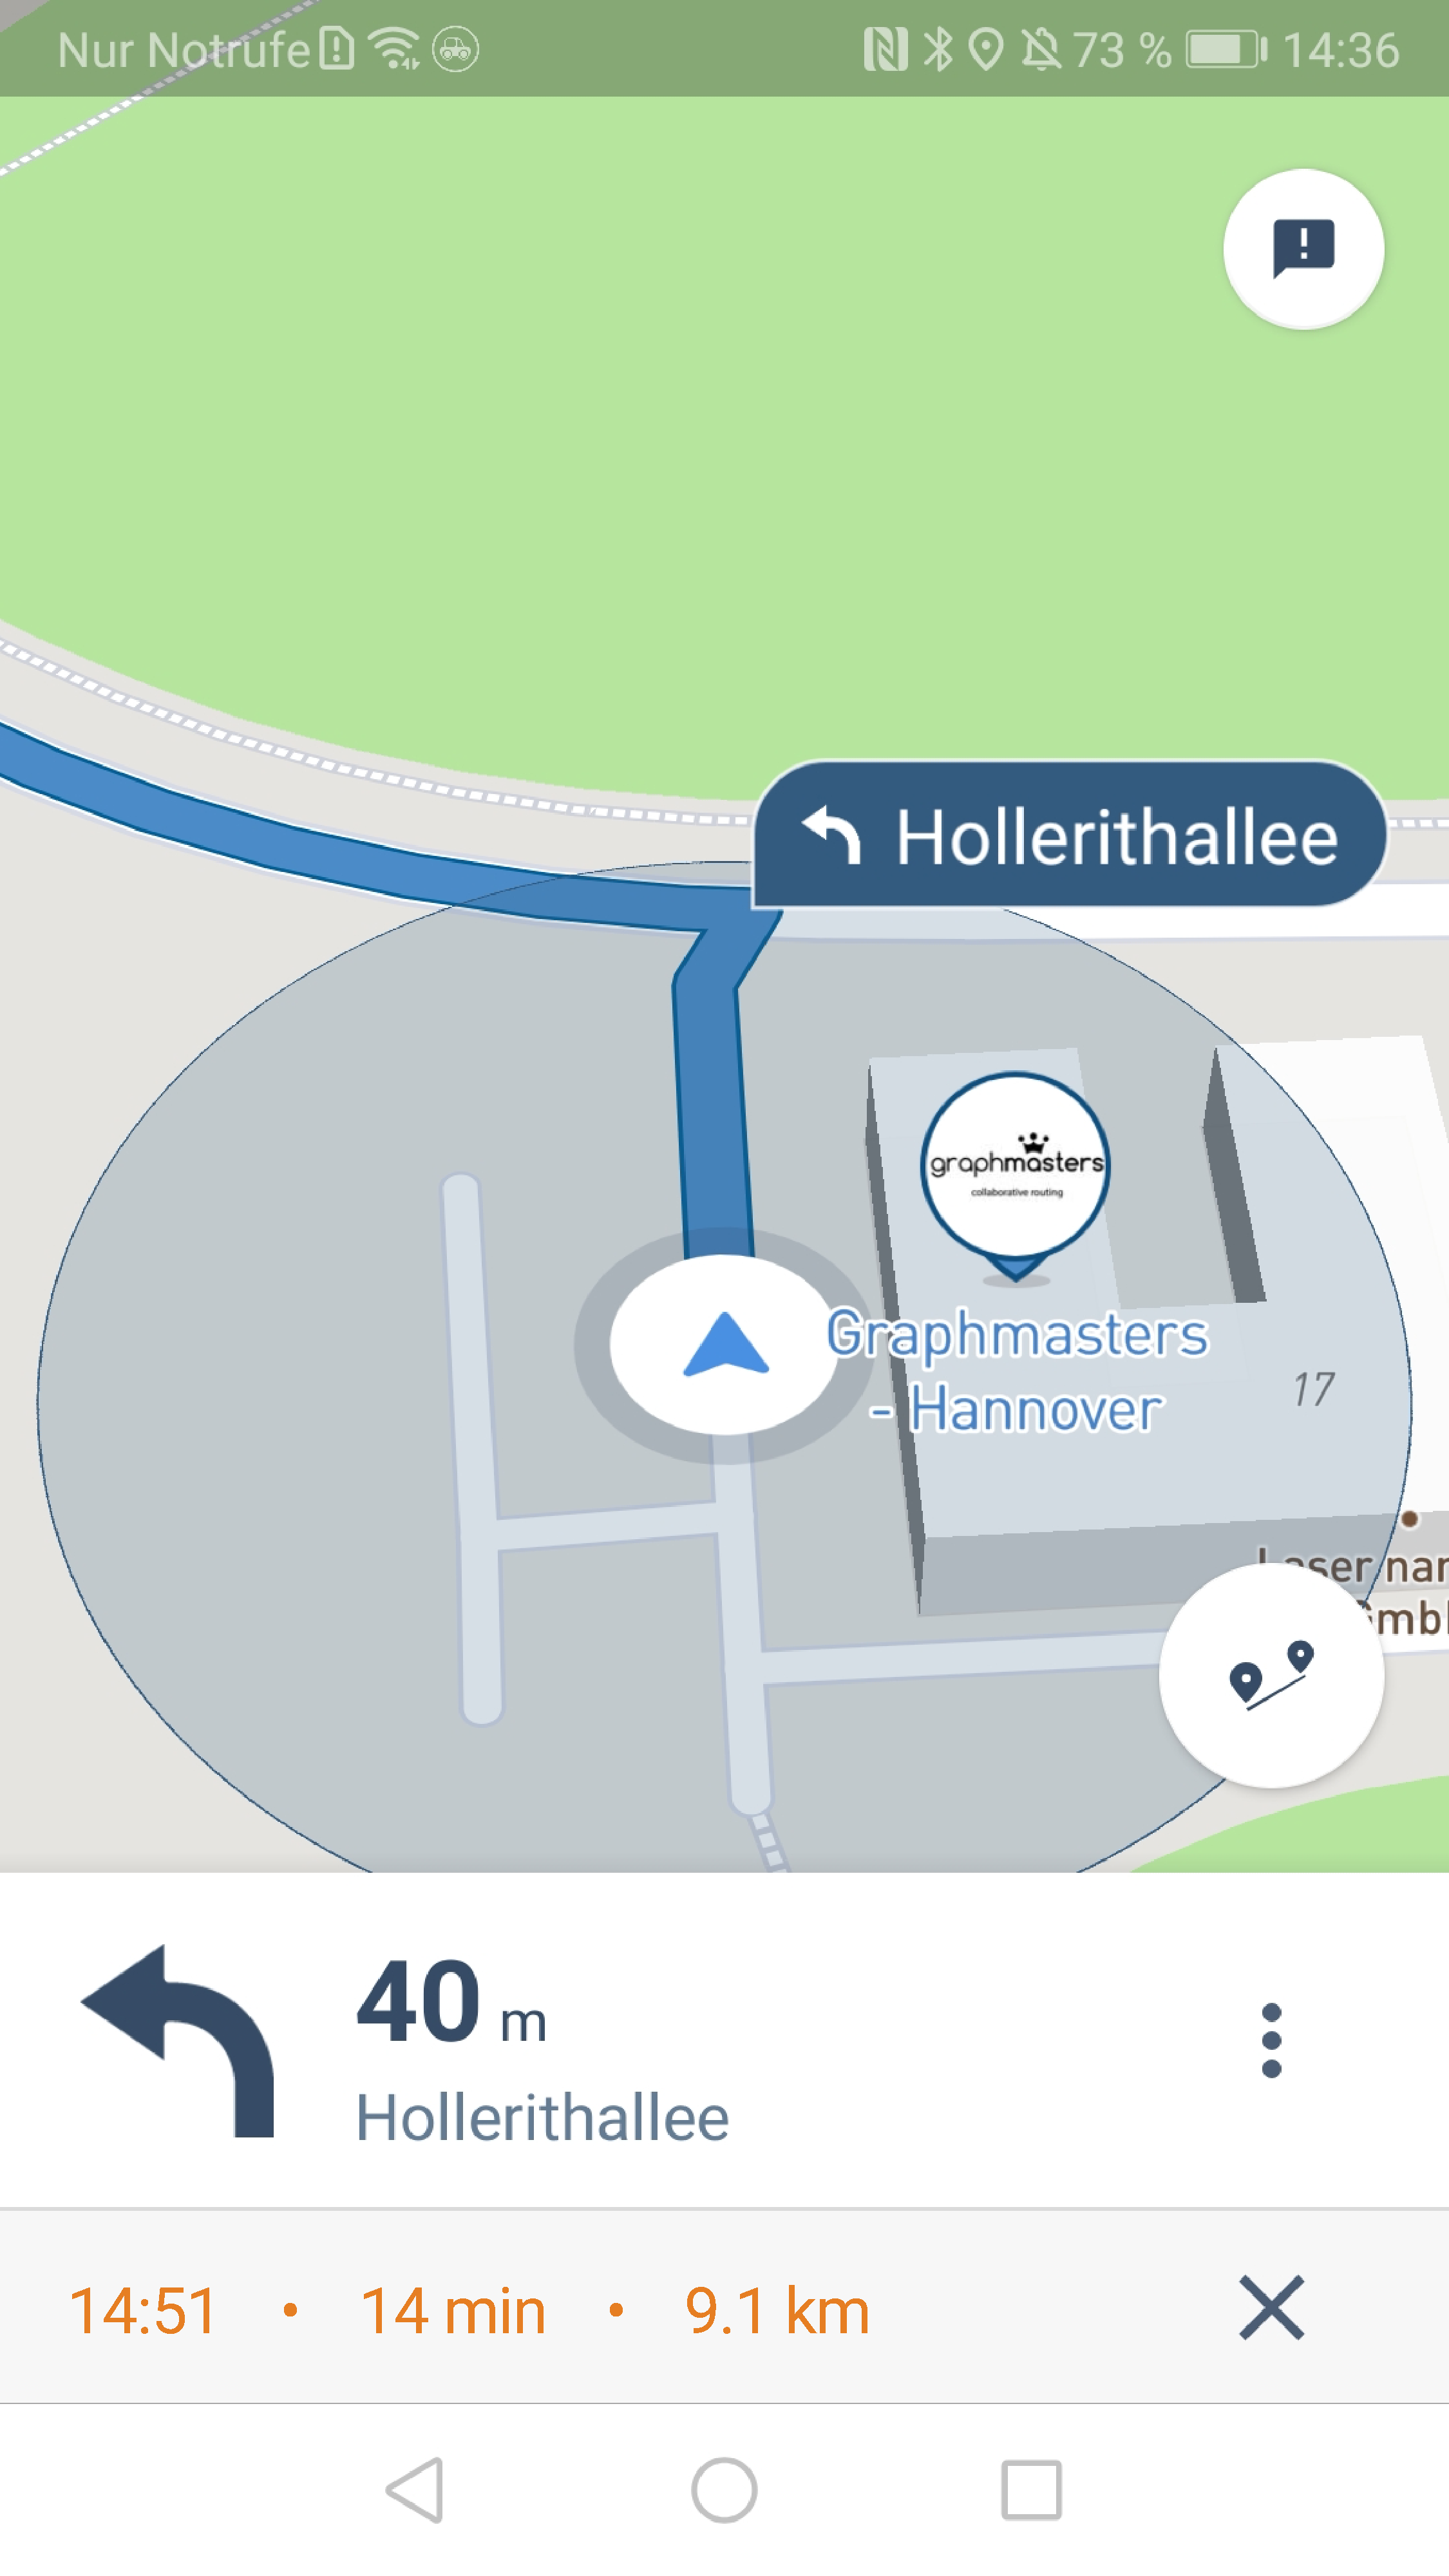
\includegraphics[width=.27\linewidth]{contents/06_model_evaluation/01_integration/res/03_traffic_volume/prototype_21.pdf}
    }
    \hspace{.055\linewidth}
    \subfloat[Alternativer Prototyp zur Positionierung der \textit{Affordance}]
    {
        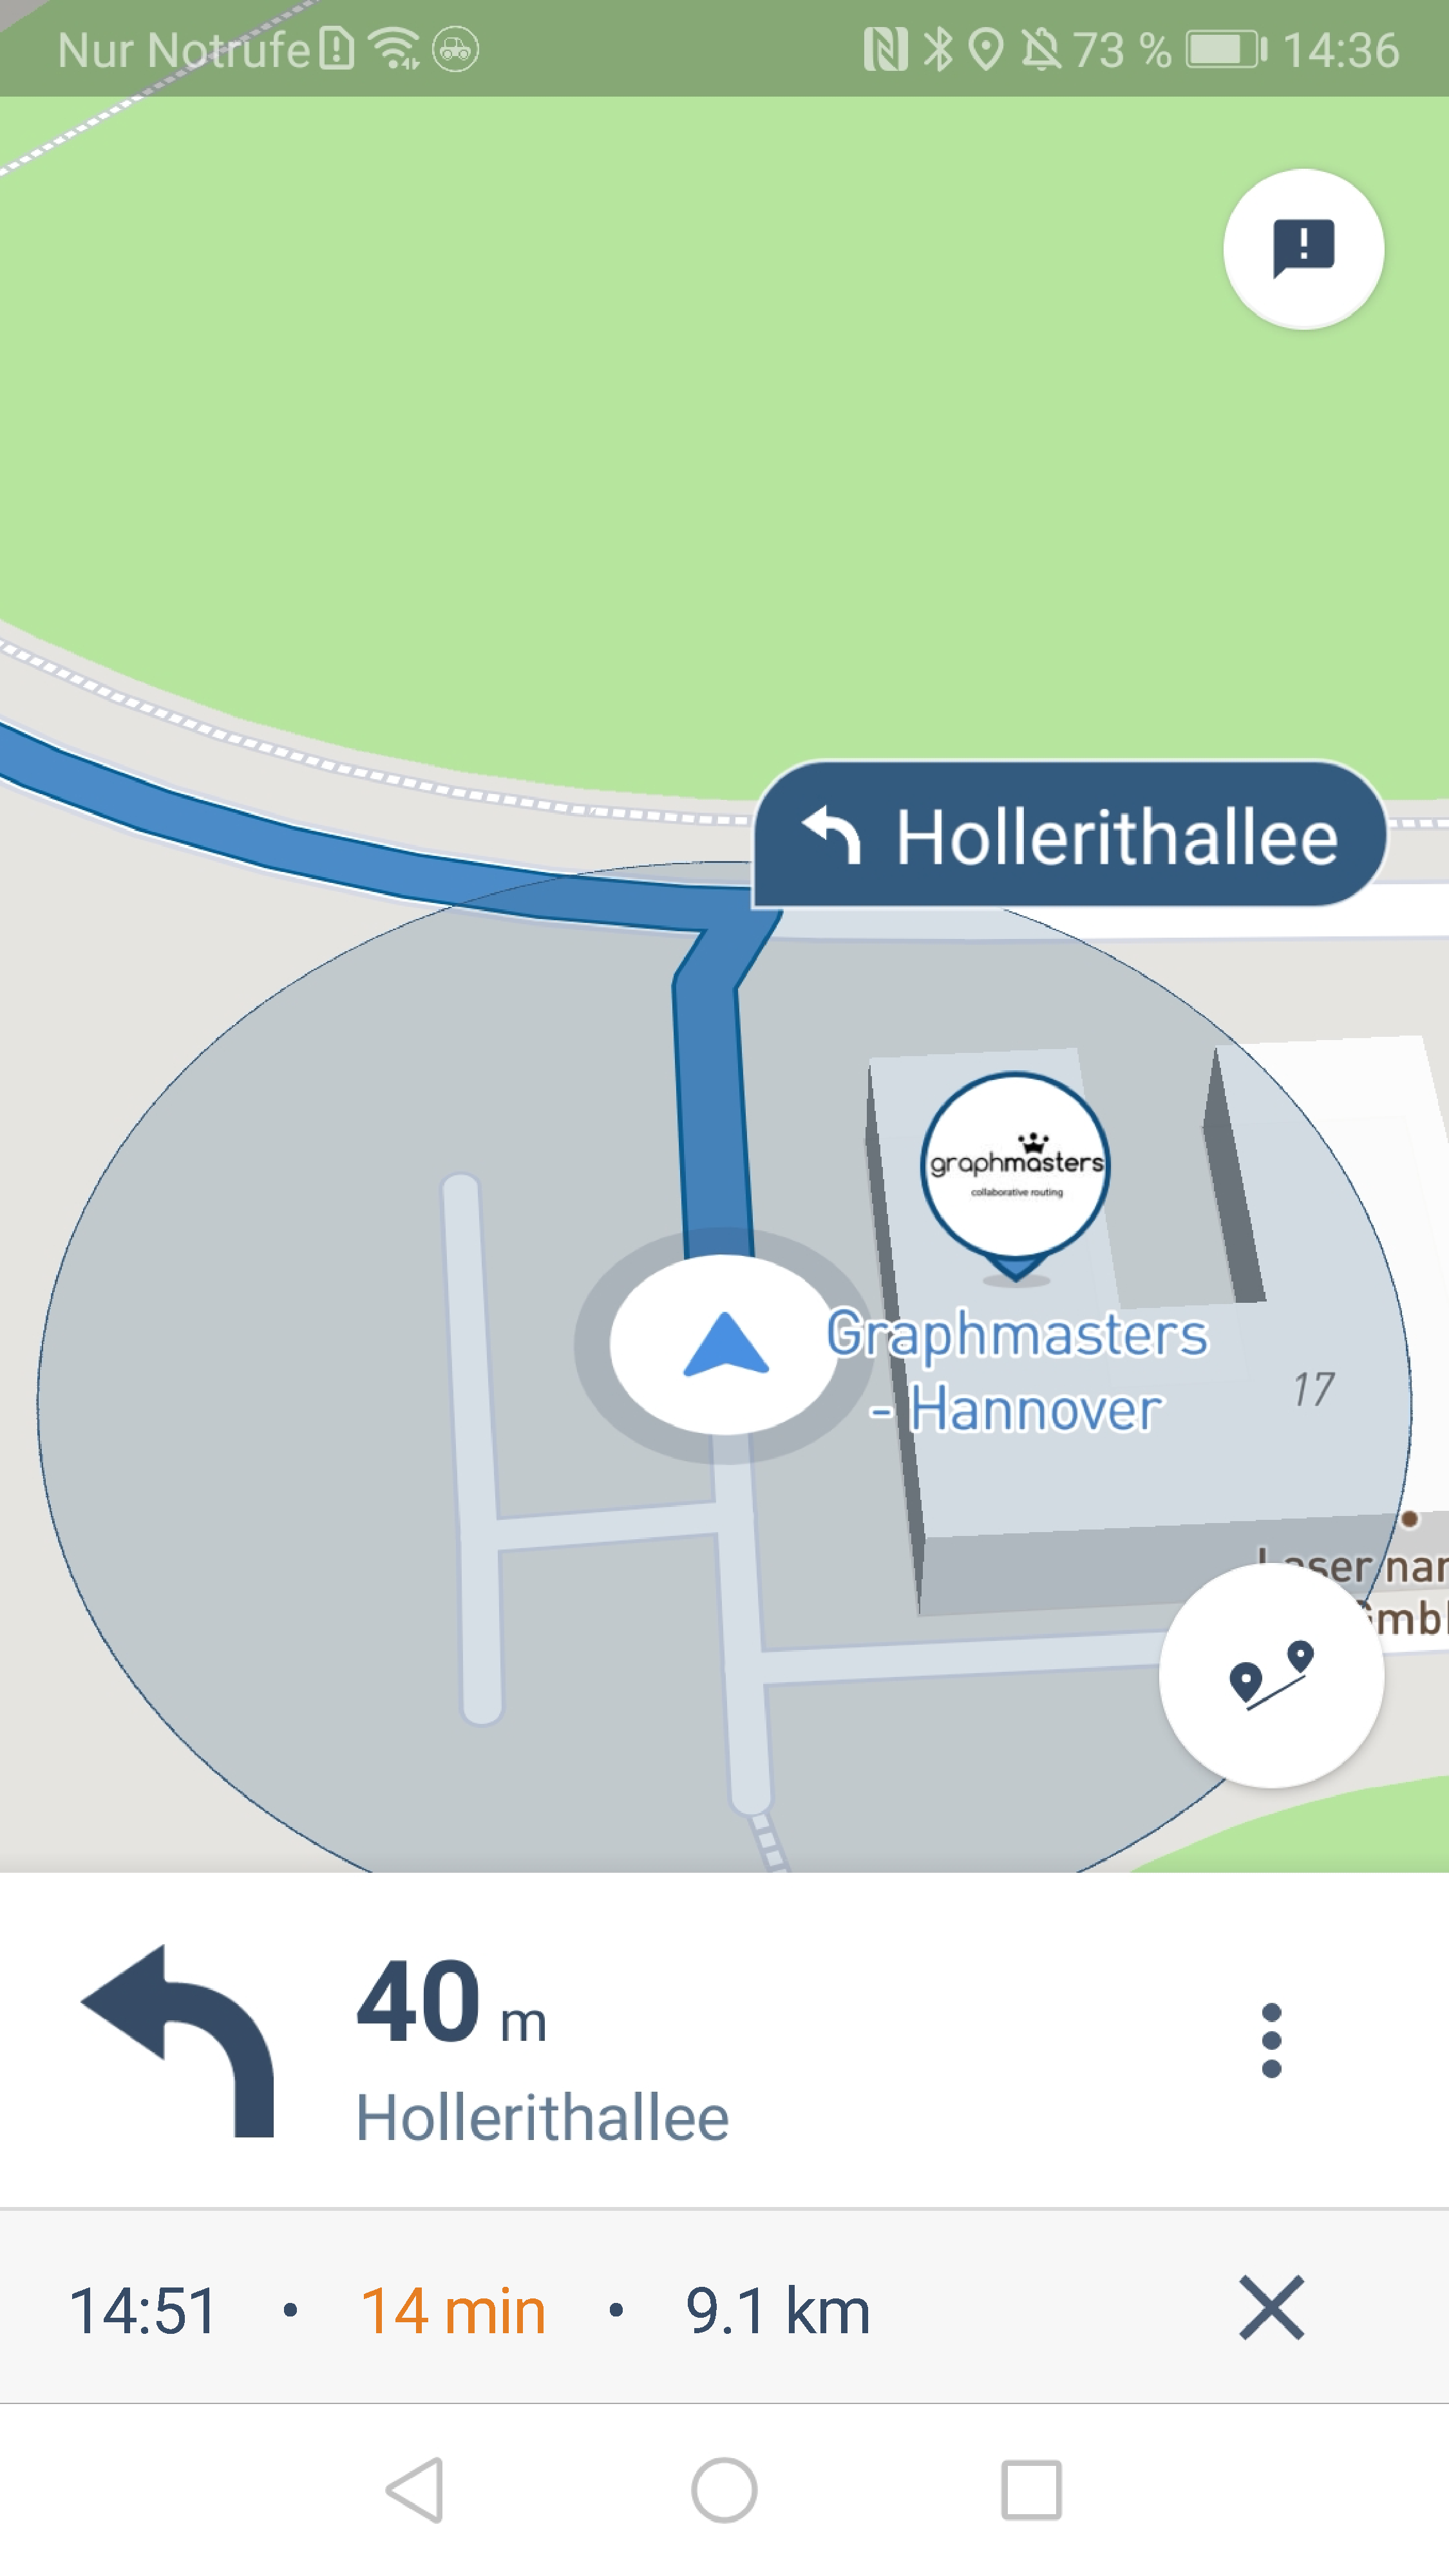
\includegraphics[width=.27\linewidth]{contents/06_model_evaluation/01_integration/res/03_traffic_volume/prototype_22.pdf}
    }
    \hspace{.055\linewidth}
    \subfloat[Finales Design der kurzen Erklärung]
    {
        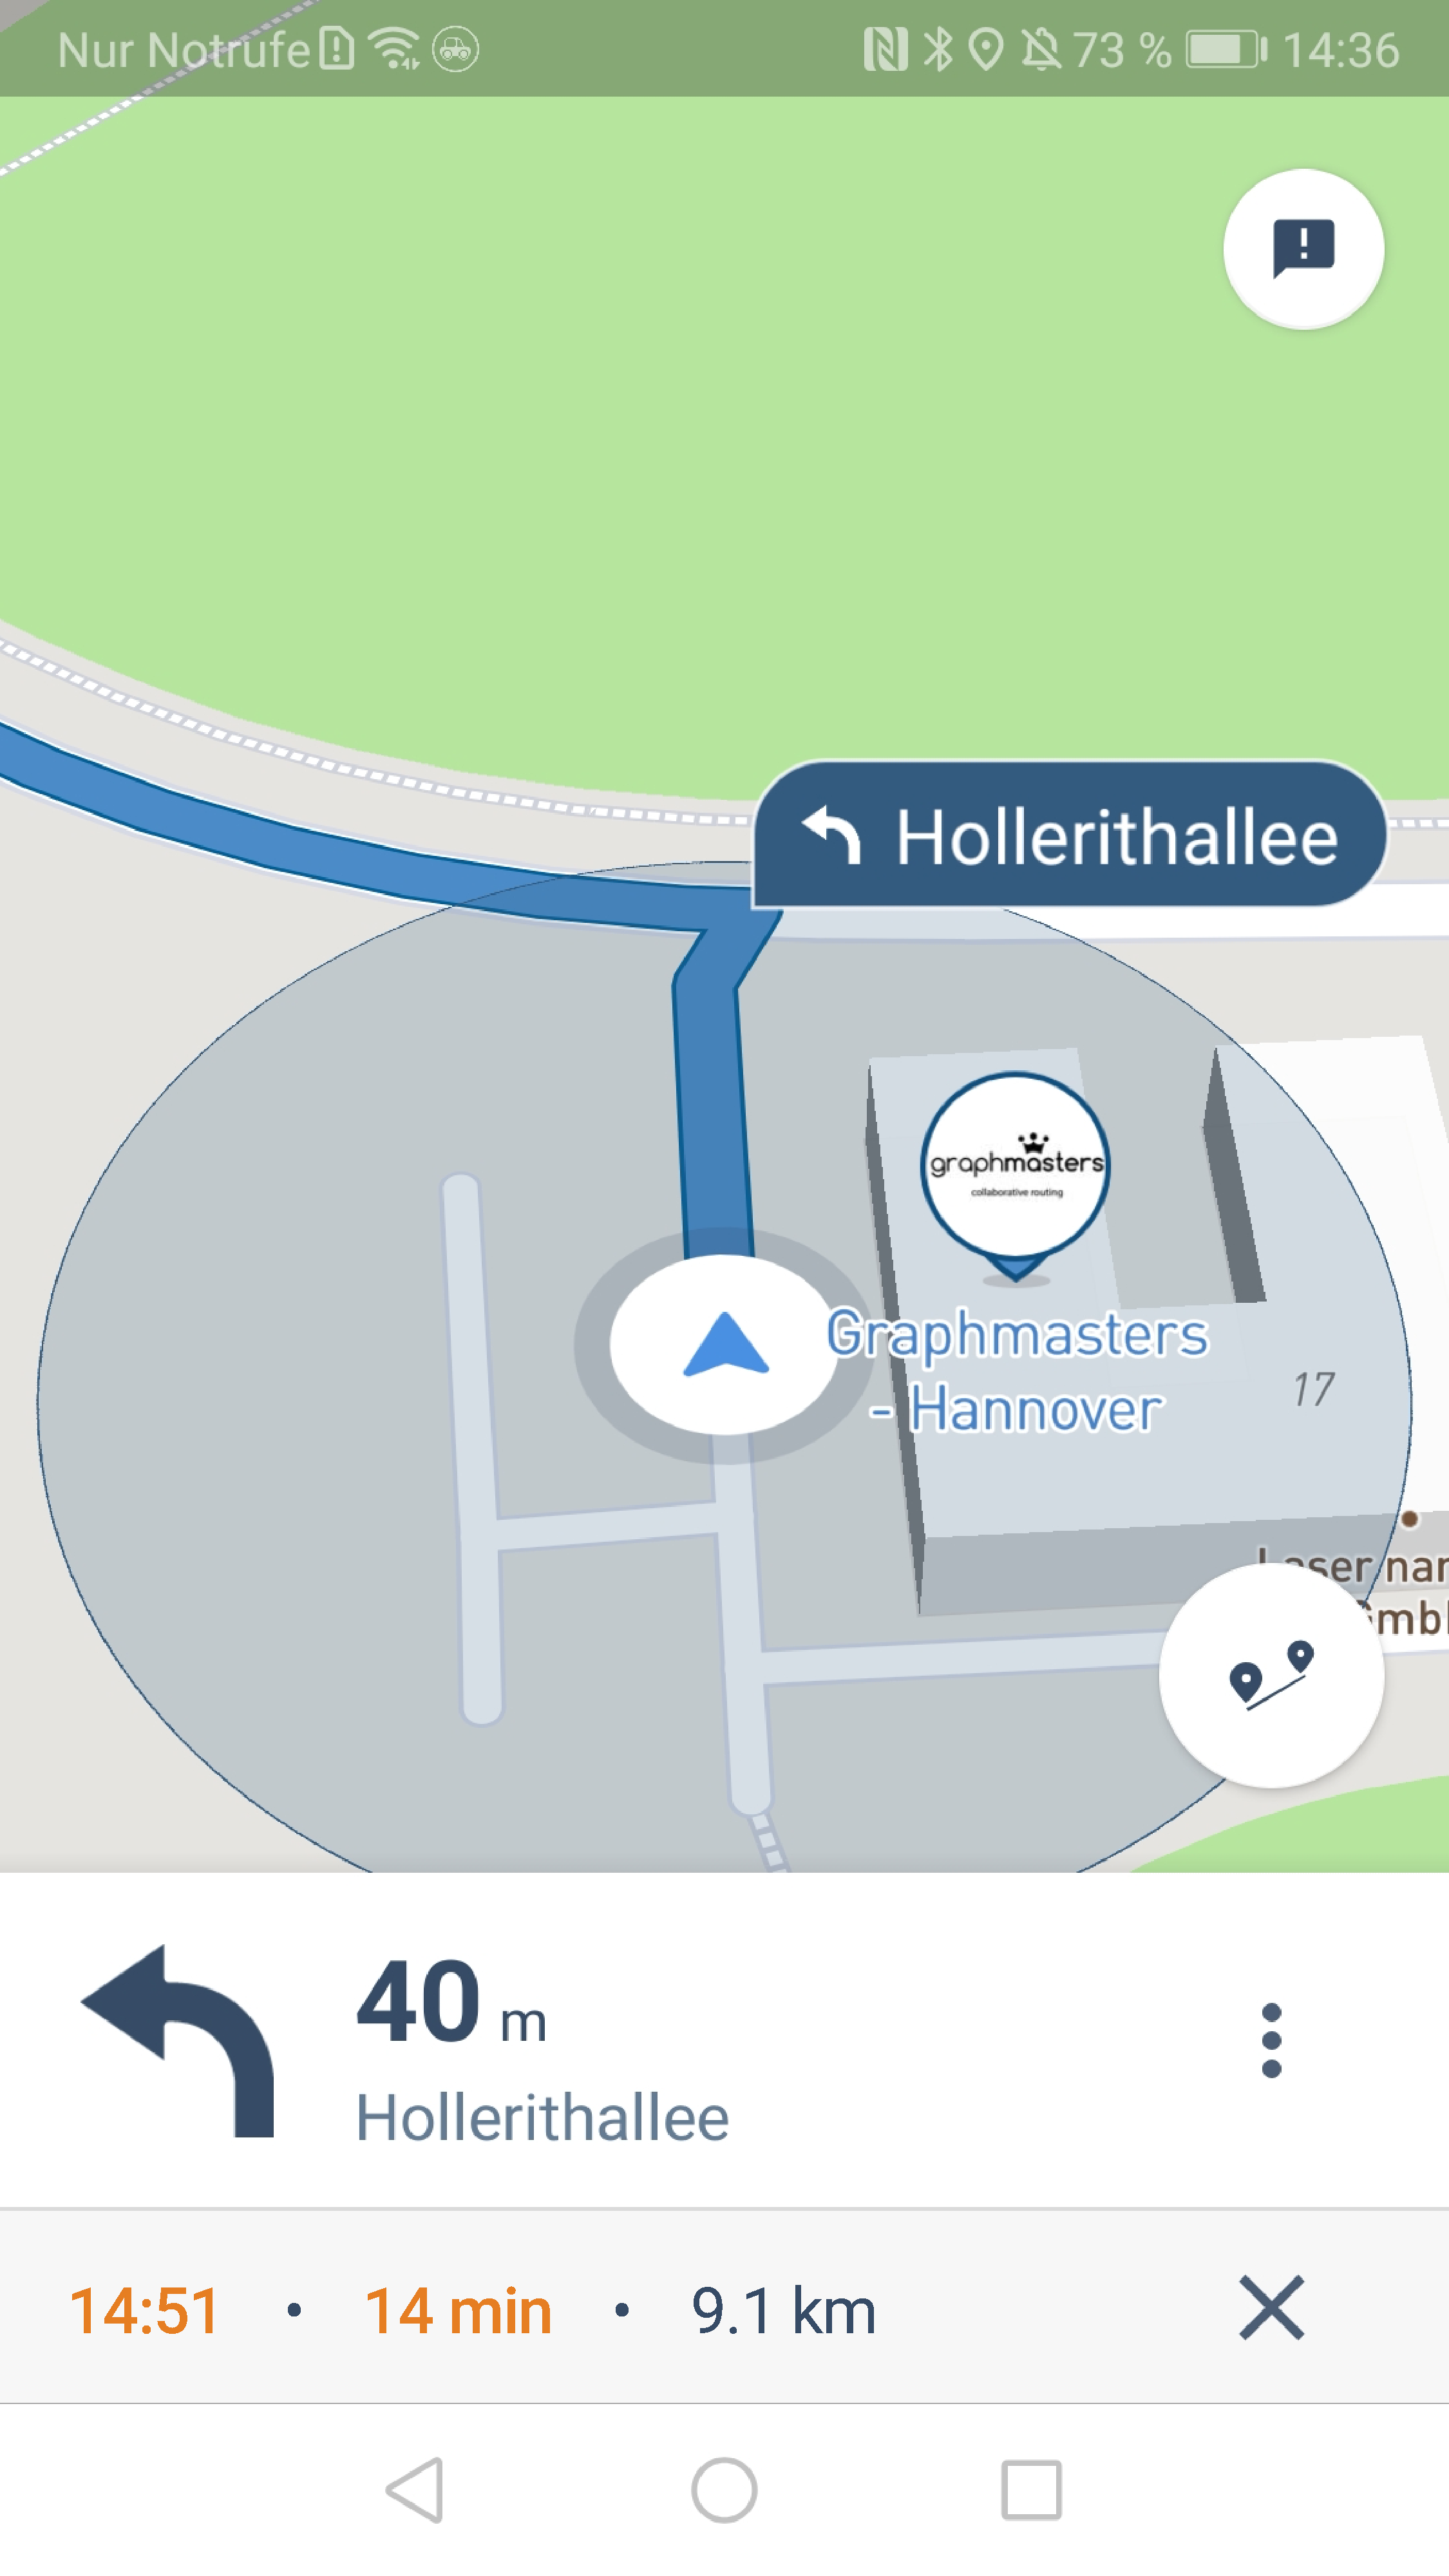
\includegraphics[width=.27\linewidth]{contents/06_model_evaluation/01_integration/res/03_traffic_volume/final_20.pdf}
    }
    \caption{Prototyp und finale Designs für die Erklärung zum kollaborativem Routing}
    \label{fig:prototype_traffic_volume_navigation}
\end{figure}

% \begin{table}[bht!]
%     \begin{tabular}{p{.25\textwidth}p{.56\textwidth}p{.1\textwidth}}
%         \hline
%         Thema & Beschreibung        & Anzahl \\
%         \toprule
%         Feature Request             & Im Review werden neue Funktionen gefordert. & 18 \\
%         \tablerowspacing
%         Kollaboratives Routing      & Das Review deutet auf ein fehlendes Verständnis, was der Grundgedanke des
%                                         kollaborativen Routings ist, hin. & 16 \\
%         \tablerowspacing
%         Schlechte Route             & Das Review enthält eine Beschwerde über eine bestimmte Routenführung. & 9 \\
%         \tablerowspacing
%         GPS-Verständnis             & Das Review deutet auf ein fehlendes Verständnis für schlechten GPS-Empfang hin. & 3 \\
%         \tablerowspacing
%         Offline-Modus-Verständnis   & Das Review deutet auf ein fehlendes Verständnis der Offline-Karten-Funktion 
%                                         hin. & 3 \\
%         \tablerowspacing
%         Fehlende Information        & Das Review enthält eine Forderung nach mehr Informationen,
%                                         die in NUNAV angezeigt werden sollen. & 3 \\
%         \tablerowspacing
%         Schlechte Suchergebnisse    & Im Review wird die Qualität der Suchergebnisse bemängelt. & 3 \\
%         \tablerowspacing
%         Verständnis Routenfarbe     & Im Review werden Nachfragen zur Einfärbung der Route gestellt. & 2 \\
%         \tablerowspacing
%         Falsche Kartendaten         & Im Review werden falsche Kartendaten bemängelt. & 1 \\
%         \toprule
%     \end{tabular}
% \caption{Anzahl der Reviews im Google Play Store und Apple App Store mit mehrfach vorkommenden Themen}
% \label{tab:06_model_evaluation_integration_app_store_reviews_overview}
% \end{table}

%\bibliographystyle{alpha}
\printbibliography

\backmatter


\end{document}